
\documentclass[11pt, oneside]{article}

\usepackage[]{graphics}
\usepackage{graphicx}
\usepackage{epstopdf}
\usepackage{hyperref}
\hypersetup{breaklinks=true, colorlinks=true, citecolor=blue}
\usepackage{natbib}
\usepackage{color}
\usepackage{soul}
\usepackage{rotating}
\usepackage{tabularx}
\usepackage{longtable}
\usepackage{lscape}
\usepackage{array}
\usepackage{multirow}
\usepackage{setspace}
\usepackage{textcomp}
\usepackage{dcolumn}
\setlength{\LTcapwidth}{6in}
\usepackage{dcolumn}
\usepackage[margin=1in]{geometry}
\usepackage{blindtext}
\usepackage[utf8]{inputenc}
\usepackage{csquotes}
\usepackage{titlesec}
\usepackage{enumitem}
\usepackage{changepage}
\usepackage[table, dvipsnames]{xcolor}
\usepackage{graphics}
\usepackage{float}



 \bibpunct{(}{)}{,}{a}{}{,}
 \doublespacing
 \raggedright
 \setlength{\parindent}{15pt} 
 \usepackage{tocloft}
%\renewcommand{\cftfigfont}{Figure }

\newcommand{\hlc}[2][yellow]{ {\sethlcolor{#1} \hl{#2}} }

\renewcommand{\labelenumii}{\theenumii}
\renewcommand{\theenumii}{\theenumi.\arabic{enumii}.}


\begin{document}
%\setcounter{secnumdepth}{0}

\hspace{5in}

\begin{center}

\LARGE{\bf Lotterhos Laboratory Handbook for Molecular Techniques
2015  }

\end{center}

\vspace{10mm}

\begin{figure}[h]
\begin{center}
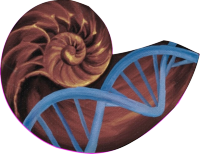
\includegraphics[height=1in]{./images/Lab_Logo.pdf}
\end{center}
\end{figure}


\renewcommand\cftloftitlefont{\Large}

\newpage 

%
\tableofcontents
%\listoftables
%\renewcommand\thesection{S1}
%\renewcommand\listfigurename{List of Supplementary Figures}
\listoffigures
\newpage
%\section{Supplementary Figures}


\section{Preface}


	This handbook is a compilation of protocols followed by the Lotterhos Laboratory members, and it is meant to transfer information among members of 	the Lotterhos lab. The original source of the protocols can be found below the title of each protocol. This handbook is not meant to replace any safety 	documentations needed to work safely in a lab. 

\newpage

\section{Introduction to the Lab}


	Welcome to the Lotterhos Lab. We work with multidisciplinary protocols that require expertise in fields such as bioinformatics, molecular science and 	marine biology. This manual has a list of the lab rules, reagent recipes and protocols used at the lab. Be respectful of the lab and follow the University 	safety rules to maintain the lab a safe shared environment. For example, keep computer areas free of chemicals. People using the computers may not 	use the same level of protection that they would use if they were to use a bench meant for chemicals. 

	This handbook should not be a limitation to the techniques that you can use in this lab. To the contrary, we expect this handbook to be a basic 			introduction to the techniques that you could use in your research. Adding or taking steps to some parts of the protocols may make some of the 		protocols more adequate to your research. As the field advances, some of these protocols may also become obsolete.  It would be an advantage to 		the lab if you update this handbook with additional protocols, notes and improved protocol versions. 

	Review your expectations and results with your lab mates and Dr. Lotterhos whenever possible. Also human error may occur, the cause of errors in 		research may come from malfunctioning machines, expired reagents, and other incidental causes. To maintain the optimal flow of a molecular lab, it is 	crucial that you and your lab-mates report any malfunctioning machines and follow the laboratory rules.  

	Your time in the lab should end with you making sure that everything is stored appropriately and that your research is documented. If you have any 		questions of the manual or of your role in the lab please ask Dr. Lotterhos.

	If you are a new member to the lab, regardless of your experience, you have to get trained in lab safety. You should check for approval from Dr. 		Lotterhos to start your lab work after you have gone through the safety training of the University, gotten familiarized with the SOP for the chemicals 		that you are planning to use, and you have gone through the checklist of Health and Safety information. 

	\newpage

	\subsection{Lab Rules}

		\begin{itemize}

			\item[--] Lab training is mandatory for all members of the lab. No work should be done in the lab without training and the approval of Dr. 				Lotterhos to initiate work. 
			\item[--] Your work in the lab should be limited to the work that you have been trained and approved to do by Dr. Lotterhos. Additional 				approval and training should be sought for any additional work outside the prior approved work.
			\item[--] Food and drink should be limited to the approved areas (outside the lab).
			\item[--] Use shoes that cover your feet (closed-toed shoes). No open-toed shoes allowed.
			\item[--] Use the protective gear required for your work.
			\item[--] Plan ahead and inform the lab members of any changes to a function of a bench. 
			\item[--] Clean your working area before and after use. If working with DNA and RNA, use 10\% of bleach to clean the bench and then 70\% 			ethanol. 
			\item[--] Gloves are meant to be used for a specific task and care should be taken not to spread contamination with gloves around the lab.  GLOVES SHOULD NEVER BE USED TO OPEN DOORS (except the fridges).
			\item[--] The main stocks are meant to be use to make aliquots for everyone`s project. You should take all of the precautions to maintain 				the main stock in optimal conditions
			\item[--] Aliquots are meant for personal use. After the use of an aliquot, the aliquot should be stored in a personal box labeled with your 				personal information.  EVERYONE HAS THEIR OWN ALIQUOT.
			\item[--] Make sure to label all of the tubes with at least the sample \#, the date and your initials. 
			\item[--] Use sterile techniques to remove supplies from a shared area. 
			\item[--] If possible, use a positive and negative control in your experiment. A positive control is a group that has been previously tested to 			work. A negative control is a group that does not have the variable being tested. These control groups are helpful because it helps you 				compartmentalize where a source of error may come from. For example, in a PCR reaction a positive control would include a DNA sample 			that has previously worked and the negative control would not have any DNA at all. The presence of a band in the negative control would 			indicate a contamination problem, and the lack of a band in the positive control could indicate a bad reagent or PCR mix problem. 
			\item[--] Use filter tips for RNA work, when training and when working with volumes of types of chemicals that may find a way to 					contaminate the pipette. 
			\item[--] Prevent contamination by closing containers as soon as you are done using them. 
			\item[--] Plan in advance and order or replenish any supply before we are out of the supply.  PLEASE PUT ORDER REQUESTS ON QUARTZY.
			\item[--] Plan to acquire all of the permits required to work with animals prior to your work.  PLAN 6-8 MONTHS FOR PERMIT AND ANIMAL CARE APPROVAL.
			\item[--] Chemicals and their waste should be discarded as mandated by their MSDS and the University rules.
			\item[--] Avoid working directly with the main stock of supplies unless you are going to make aliquots. Aliquots should be made with the 				minimal amount of reagent needed for a few reactions. Aliquots maintain your reagents fresh and reduce contamination problems. When you make chemicals, please label with date and your initials.
			\item[--] Put autoclave tape on everything that has been in the autoclave.
			\item[--] Pay attention to glass thermometers - there are 3 levels of immersion (35mm to full immersion), and IT MATTERS
			\item[--] ITEMS FALLEN TO THE FLOOR: The floor is contaminated with PCR product transferred on the shoes of individuals coming from the post-PCR area; therefore, anything falling to the floor must be treated as contaminated. Disposable items that have fallen to the floor, such as empty tubes, pipette tips, gloves, lab coat hangers, must be discarded. Non-disposable items that have fallen to the floor, such as a pipette or an important sample container, must be immediately and thoroughly cleaned with a 0.5\% Sodium Hypochlorite (10\% Bleach) solution to remove PCR product contamination. Clean any lab surface that has come in contact with the contaminated item. Individuals handling anything that has fallen to the floor, disposable or non- disposable, must discard their lab gloves and put on a new pair.
		\end{itemize}

	\newpage

	\subsection{Lab Expectations}

		\begin{itemize}


			\item[--] THAT YOU DO NOT FABRICATE DATA.  Above all else, this is my most basic expectation.
			\item[--] THAT YOU HAVE FUN, ARE POSITIVE, AND BE PART OF THE TEAM!  Science is fun when we work as a team.  When one project 			does not turn out as expected, I expect everyone to reflect internally on how they could have helped the team prepare better.  Although it is 			impossible to forsee all possible outcomes of an experiment, I expect everyone to have a positive attitude and be persistent in the face of 			difficulty. There is always a reason when something isn`t working.
			\item[--] That you communicate when you do not fully understand something, or when you make a mistake.  It is easier to forgive an honest 			mistake than a one who pretends to understand.
			\item[--] That you read the literature relevant to your project, and you do not completely rely on other`s expertise.
			\item[--] That you pick up and clean up after yourself before you leave for the day.
			\item[--] That you maintain a meticulous lab notebook AND online open notebook documenting your activities related to the lab.  Starting in Fall 			2014, all lab notebooks are to be kept in the lab.  You lab notebook contains original data that is necessary to preserve in the interest of 				repeatability in science.  I prefer that you make copies if you need information in the notebook, and only check the notebook out when you 			need to add to it.
			\item[--] That you read the Material Safety Data Sheets for all chemicals that you will be using in the lab, BEFORE you use them.  I expect that 			you will make yourself aware of how to handle and dispose of hazardous chemicals, and what to do in the event of a chemical spill.
			\item[--] That you use a pipette correctly and you do not contaminate them.  This includes knowing how to use the first stop on the pipette 			correctly, and how to check the tip and make sure there is no air bubbles in it.  That you autoclave pipettes on a regular basis.
			\item[--] That you put gloves on before you touch anything that is autoclaved.
			\item[--] That you put gloves on before you handle any hazardous chemicals.
			\item[--] That you are familiar with the locations of eye wash, safety shower, and fire extinguisher.  I also expect that you will be familiar with 			Environmental Health and Safety standards, and receive appropriate training when necessary.
			\item[--] That you do not touch door handles or walk around the building with gloves on.  If you need to carry something hazardous, please 			wear a glove in one hand and use the ungloved hand to open doors.
			\item[--] That when you are using an expensive and sensitive piece of equipment (i.e., the CO2 analyzer, the mass flow controllers, the 				pipettes, the scales, the pH meter, etc.), you make yourself aware of the cost of that equipment, and are careful not to exceed the 					parameter range for that equipment.  For example, flow to the CO2 analyzer cannot exceed a certain amount.  Likewise, overloading a 				sensitive scale can cause harm.
			\item[--] That when working with seawater, you understand that EVERYTHING needs to be rinsed in freshwater before you pack up for the 			day. This is especially true for knives, needles, pliers, forceps, and anything else that is steel (even stainless steel will start to rust).  Plastic 			will get brittle after prolonged use in seawater.
			\item[--] That with working with spawning invertebrates, you rinse your hand after you touch a male.  This is important to prevent the 					contamination of pesky sperm to other males and females.
			 \item[--] Finally, I expect that you think through what you are (or the team is) going to do and be prepared before you start.  The exemplary 			team member is not the one that simply follows directions-it is the one that has thought through every step, researched multiple avenues, 			and is prepared.   

		\end{itemize}

	\newpage

\section{What You Should Be Keeping Track of In the Lab And Your Lab Notebook}
	\begin{enumerate}
		\item Everything you do
		\item How many boxes of tips you use
		\item How many uL, mL, or mg of expensive reagents.  If you are unsure of reagent cost, please check online or on Quartzy.
		\item How many items in a kit.  E.G. Qiagen DNAeasy, cassettes of the Pippin, Bioanalyzer chips, Kapa Illumina adapter kits, etc...
		\item Whenever you use a piece of equipment to do something, note the model number in your lab notes and open notebook posts.		
	\end{enumerate}
		
\section{Lab Calendar}
	\begin{enumerate}
		\item AUGUST, ANNUALLY: pipette calibration
		\item AUGUST, ANNUALLY: freezer defrost
		\item LAST WEEK OF EVERY MONTH: CLEAN UP.  This clean up is mainly to reduce any contamination. I hit the common used areas with bleach and alcohol, and I try to improve any situations that may lead to contamination (sterilize shared containers, re-organized areas that are being problematic, etc).  Acid wash all of the plastic containers that are autoclavable and are used to carry RNA or DNA. Use a 10\% Hydrochloric acid (and wear all of the protection needed). Autoclave pipettes.  Wash glassware in detergent and rinse thoroughly.
		\item FIRST WEEK OF EVERY MONTH: REMIND Dr. L TO DO THE MONTHLY BUDGET.  A copy of all receipts from the previous month should be sent to Heather.
		\item WEEKLY: backup and update computers
		\item WEEKLY: chart of freezer temperatures	
		\item DAILY: CLEANING: Note: To prevent sample or reagent degradation, make sure that all vapors from the cleaning solution have fully dissipated before beginning any processes.  A daily cleaning of thearea using a 0.5\% Sodium Hypochlorite (10\% Bleach) solution helps to eliminate PCR product that has entered the pre-PCR area, and reduces the amount of PCR product in the post-PCR area.
Identify areas that pose the highest risk of contamination, and clean these areas with a 0.5\% Sodium Hypochlorite (10\% Bleach) solution before beginning any pre-PCR processes. High-risk pre-PCR areas might include, but are not limited to: Bench tops, Door handles, Refrigerator/freezer door handles, Computer mouse, Keyboards.  High-risk post-PCR areas include those above and: Thermal cyclers, Bench space used to process amplified DNA.		
		
	\end{enumerate}
	\newpage
	

\section{Lab Online Accounts}
	\begin{enumerate}
		\item beckman coulter (ampure beads) - 
		\item agilent - k.lotterhos, lab password
		\item qiagen - 
		\item sigma aldrich - k.lotterhos, lab password
		\item VWR - lab password
		\item bioexpress (k.lotterhos@neu.edu, lab password) (always have trouble with paying credit card on their site)
		\item Kroll - identity protection - k.lotterhos, biennium
		\item Zymo Research Account (username: k.lotterhos  lab password
)
		\item airgas - k.lotterhos@neu.edu, lab password
		\item Fisher NLSU pin: 4956 (expires ~March 1, 2016)
		\item Eppendorf, k.lotterhos,  lab password, Currently have ~\$4000 to spend in ecredits
	\end{enumerate}
	\newpage

\section{Lab Manager (RA) Responsibilities}
	\begin{enumerate}
		\item Order supplies, be aware of deals and when they expire.
		\item Manage QUARTZY web inventory and keep it up to date.
		\item Manage lab safety and compliance programs including mandatory training of all lab members
		\item Oversee management of the laboratory collections of protocols \& procedures
		\item Train students and lab members in general in a variety of laboratory procedures
		\item Maintain a lab calendar with equipment needs of inspection or calibration
		\item Keep lab documents organized
		\item Write meticulous directions for new protocols
		\item Keep samples organized in the freezer
		\item Once per week check on equipment, if anything is broke take steps to check on warranty and contact reps.
		\item Sterilize tips, tubes, and other consumables for all lab users. 	
		\item Daily cleaning
	\end{enumerate}
	\newpage

\section{Prevent PCR Product Contamination}
Note that our lab isn't really set up to do this.  But these are important considerations.

The PCR process is commonly used in the laboratory to amplify specific DNA sequences. Unless proper laboratory hygiene is used, PCR products can contaminate reagents, instrumentation, and genomic DNA samples, causing inaccurate and unreliable results. PCR product contamination can shut down lab processes and significantly delay normal operations.
Make sure that the lab is set up appropriately to reduce the risk of PCR product contamination:
	\subsection{ Physically Separate Pre-PCR and Post-PCR Areas}
		\begin{itemize}
			\item Physically separate laboratory space where pre-PCR processes are performed
(DNA extraction, quantification, and normalization) from the laboratory space where PCR products are made and processed during the (post-PCR processes).
			\item Never use the same sink to wash pre-PCR and post-PCR troughs.
			\item Never share the same water purification system for pre-PCR and post-PCR
processes.
			\item Store all supplies used in the protocols in the pre-PCR area, and transfer to
the post-PCR area as needed.
		\end{itemize}
	\subsection {Use Dedicated Equipment and Supplies	}
		\begin{itemize}
			\item Dedicate separate full sets of equipment and supplies (pipettes, centrifuges, oven, heat block, etc.) to pre-PCR and post-PCR lab processes, and never share between processes.
			\item Dedicate separate storage areas (freezers and refrigerators) to pre-PCR and post-PCR consumables.
		\end{itemize}
			
Because the pre- and post-amplification reagents are shipped together, it is important to unpack the reagents in the pre-PCR lab area, and then move the post-amplification reagents to the proper post-PCR storage area.
	


\section{Health and Safety Information}

	Checklist 

	Please make sure to follow the steps noted below before you start your lab work: 

	\begin{enumerate}
		\item \hl{Complete the following safety trainings online: 
		list here}
		\item Read the SOP for all chemicals you use but especially the following chemicals:
		- Formaldehyde (corrosive)
		- Mercuric Chloride. 
		-EtBr
		
		\item Get a Research Laboratory Training of the Lotterhos Lab.
		\item Get approval from Dr. Lotterhos.

	\end{enumerate}

	\newpage

\section{Resources for the Molecular Biologist}

	\begin{enumerate}

		\item The Simple Fool\textquotesingle s Guide to PCR (Palumbi) (in this folder)
		\item Molecular Zoology: Advances, Strategies and Protocols (Ferraris and Palumbi)
		\item Roche PCR guide (in this folder)

	\end{enumerate}

\newpage




\section{Lab Equipment Information/Tips}

	\subsection{pH Meter Operation Tips}

		(adapted from the BITC2441 Lab Manual Fall 2011)
	
		\begin{center}
	
			\hspace{1in}
	
			Small errors in the pH adjustment of a buffer can have large effects on sensitive reagents used in the molecular lab. There are many things 			that you can do to improve the performance of a pH meter. 
	
		\end{center}		

		\begin{enumerate}		
			\item Never assume that a pH meter is in calibration. Even when properly maintained and cared for, a pH meter undergoes considerable 				drift in a matter of hours after calibration. Follow the appropriate SOP to determine whether your pH meter is in calibration and to bring it 				into calibration. The standard buffers used to calibrate a meter should bracket the pH of the sample to be measured. Use standard solutions 			to calibrate the pH meter. Note that the pH of the buffer depends on temperature.  So after calibration, sometimes the pH meter reads a 				value that is different than the buffer because of temperature (i.e. 7.04 instead of 7.00). You may need to check a chart to see if the reading 			on your buffer is correct for the temperature of the liquid.
			\item Verify that the standard buffers that you are using have not expired. This is especially important for pH 10 buffer, where CO2 dissolved 			from the air will cause the pH to go down over time. 
			\item Avoid direct contact of solids or surfaces on the bulb of the pH electrode as it has a very fragile membrane. The electrode should not 			be wiped dry because static discharge can build up on the electrode. 
			\item Follow the manufacturer instructions for the proper care and use of an electrode. MOST electrodes, such as gel-filled electrodes, 				should be stored in pH storage solution (this is typically pH 4.0 buffer), and will be ruined if stored dry. 
			\item The best indicators of the electrode condition are the slope of the calibration curve and response time required to obtain a stable pH 			reading. As any electrode ages, the slope decreases from 100\%. The recommended operating range varies by manufacturer but is usually 			92 - 100\%. The response time will become longer as the sample components coat the sensing glass bulb with continued usage. This can 			often be remedied with cleaning and/or replacing the filling solution, following the manufacturer directions. 
		\end{enumerate}

	\newpage




\section{Reagents}

	\subsection{Reagent Preparation Tips}

		(adapted from the BITC2441 Lab Manual Fall 2011)

		\hspace{1in} The ability to make reagents is an essential skill. The accuracy of calculation and of measurement is critical to the outcome of any 		experiment, whether it be one you do yourself or one in which you prep for someone else. There are several critical aspects to making solutions 		that should be followed at all times.  

		\begin{itemize}

			\item Check and recheck each calculation. It is best if two people make a calculation independently and then cross check their answers.  
			\item Read each reagent bottle twice, once before using and once afterwards. This helps ensure that the right reagent is used.  
			\item Write down the solution prep for every reagent that you make. Ideally this should include the formula, the supplier and catalog number 			if available, as well as the concentration, the expiration date of the chemical, when it was received, how it was stored upon receipt, and the 			amount weighed out for each reagent. If the pH is adjusted or the solution is sterilized, information about these procedures should be 				documented. Some solution prep forms will also have space to include the balance number, pH meter number and other pieces of 					important information. The storage conditions for the solution that was prepared should also be recorded here.  
			\item Label each solution bottle before filling. Write down the name of the solution, its concentration, its pH if it is a buffer, your initials, the 			control \# assigned to the solution (if any), and the date. Some industries have special blank labels to be used for each reagent. Others use 			tape and a permanent marker. There are labeling software programs and systems for labeling and making electronic records for solutions 			prepared in laboratories.  
			\item Record any changes observed in materials during solution preparations, no matter how trivial they might seem. This includes the 				formation of gas bubbles and any change in color. This record can be used to trace back a problem to its source quickly and easily or to 				confirm that a problem does not lie in the reagents or their preparation.

		\end{itemize}

	\newpage

	\subsection{Aliquots}

		Aliquots are smaller portions of the reagents to be used that are divided into smaller containers. Aliquots act as a safety net in your molecular 			work by preventing contamination and to minimize the number of times your reagents are frozen-thawed. 

		The volume of the aliquots should be enough for a few samples / reactions. Aliquots of small volumes will keep you changing your aliquots and 		therefore minimizing your chances of contamination and of exposing your reagent to repetitive freeze-thawing. An additional good practice would 		be to not use the same pipette tip between an old and a new reagent. 

		The use of aliquots also creates an environment that is friendly for beginners. Aliquots allow everyone to start with high quality reagents by 			preventing contamination from shared use. If you feel like you may have made an error that could have caused a contamination, or things are 			not working well (maybe one reagent went bad because of high temperatures) - then throw your aliquots away and start with fresh ones! 

		You can make aliquots of your samples too! Aliquots of your samples are often called working stocks. For example: I have 30ul of DNA from an 		extraction. DNA extractions often are of high concentrations ($>$ 300 ng/ul), so I make aliquots of 1:5 or 1:10 DNA dilutions. This allows me to 			have at least one main stock of uncontaminated samples for my future use or for the lab use. 

		\vspace{3mm}

		\hspace{1in} Aliquots should:

		\begin{itemize}
			\item have a label with name, concentration and date
			\item be made from an original source that is clean and of optimal quality
			\item be made in a clean environment. Try to think about your work, your labmates work, and of potential future work. For example: working 			with barcodes genes would be a pain if your aliquots already come with fungi spores. 
			\item whenever possible try to take additional steps to guarantee the quality of the aliquots. For example: starting with high water quality 				may not be enough once you have exposed the aliquot to the environment - You can always pass the water aliquots through UV light
		\end{itemize}


	\subsection{Reagent Recipes and Ordering Information}



		\hspace{5mm}{\bf 7.5M ammonium acetate}

			\hspace{2mm}ammonium acetate	(Fisher \#A637500) \hspace{5mm}		57.81g

			\hspace{2mm}water							(to a final volume of 100ml)

			\hspace{2mm}*If needed, sterilize by filtration in 0.2um filter. 

			\hspace{2mm}*final pH will be 5.5

		\vspace{5mm}

		{\bf Bleach 10\%}

			\hspace{2mm}Bleach\hspace{10mm}	10ml

			\hspace{2mm}DI Water\hspace{6mm}		90ml

			\hspace{2mm}*solution is good for up to 7 days

		\vspace{5mm}

		{\bf 0.5M EDTA (pH - 8)}

			\hspace{2mm}Disodium ethylenediamine tetraacetate 	(Fisher \#BP120500)\hspace{3mm}		186.1g

			\hspace{2mm}Water\hspace{95mm}												80ml

			\hspace{2mm}NaOH\hspace{55mm}	(Fisher \#BP359-212) \hspace{1mm}	18g

			\hspace{2mm}*Stir vigorously on a magnetic stirrer. Adjust the pH to 8.0. Sterilize by autoclaving

		\vspace{5mm}


		{\bf 1mM EDTA (pH - 8) for storing extracted RNA}
		EDTA should help stabilize and protect the RNA.  Use sterile 25mL pipettes to measure RNA free water and put into a 100mL glassware (autoclaved, wiped clean with RNAaseZap or RNAase Away, and rinsed with RNAase-free water).  Clean magnetic spinbar with RNAaseZap.  Calibrate pH meter an wipe outside with RNAase zap.  Use pasteur pipette to add HCl for pH adjustment, but wipe outside with RNAase-Zap.

			\hspace{2mm}Disodium ethylenediamine tetraacetate 	(Fisher \#BP120500)\hspace{3mm}		0.372 g

			\hspace{2mm}Water\hspace{95mm}												80ml

			\hspace{2mm}NaOH\hspace{55mm}	(Fisher \#BP359-212) \hspace{1mm}	0.036 g

			\hspace{2mm}*Stir vigorously on a magnetic stirrer. Adjust the pH to 8.0. Sterilize by autoclaving

		\vspace{5mm}
		
		
		{\bf Ethidium Bromide (10mg/ml)}

		\noindent {\bf CAUTION:} Ethidium bromide is a mutagen and is toxic. Wear gloves when working with ethidium bromide solutions and a mask 			when weighting the powder. 
		
		\vspace{2mm}
		
			\hspace{2mm}Ethidium bromide (Fisher \#BP1025)	\hspace{2mm}1g

			\hspace{2mm}Water\hspace{56mm}100ml

			\hspace{2mm}*stir on magnetic stirrer for several hours to ensure that the dye has dissolved

			\hspace{2mm}*light sensitive, wrap the container in aluminum foil or transfer to a dark bottle

			\hspace{2mm}*store at 4C

	\newpage

		{\bf CTAB}									

			\hspace{2mm}4M NaCl \hspace{67mm}(Fisher \#S271-1)	\hspace{12mm}	35ml

			\hspace{2mm}0.5M EDTA pH 8.0 \hspace{49mm}(Fisher \#BP120500)\hspace{9mm}4ml

			\hspace{2mm}1M Tris-HCl pH 8.0\hspace{92mm} 10ml

			\hspace{2mm}CTAB (Cetyl Trimethyl-Ammonium Bromide)\hspace{5mm}	(Fisher \#AC22716100)	\hspace{2mm} 2g

			\noindent*Mix ingredients together in a clean beaker. Stir on hot plate with stir bar. Heat gently until CTAB is dissolved. Pour into 				graduated cylinder and bring volume up to 100ml using nanopure H2O. Pour into a bottle with a cap. Autoclave before using. Store at room 			temperature. Discard after 1 year. 

		\vspace{5mm}

		{\bf dNTPs (10mM)}

			\hspace{2mm}To make 48 aliquots of 25ul each of 10mM dNTPs

			\hspace{2mm}All of the items below come in a Fisher package \#FERR01811

			\hspace{40mm}			12X	 \hspace{5mm}	1X
			
			\hspace{2mm}dTTP (100mM)	\hspace{9mm} 120ul	\hspace{5mm}	10ul

			\hspace{2mm}dATP (100mM)	\hspace{9mm} 120ul	\hspace{5mm}	10ul

			\hspace{2mm}dGTP (100mM)	\hspace{9mm} 120ul	\hspace{5mm}	10ul

			\hspace{2mm}dCTP (100mM)	\hspace{9mm} 120ul	\hspace{5mm}	10ul

			\hspace{2mm}ddH20 \hspace{25mm}		720ul	\hspace{5mm}	60ul
	
		\vspace{5mm}

		{\bf 5M NaCl 500ml}

			\hspace{2mm}NaCl	\hspace{5mm}  (Fisher \#S271-1) \hspace{3mm} 146.1 g

			\hspace{2mm}H2O 		\hspace{40mm}			$\sim$350 ml 

			\hspace{2mm}*Dissolve, then bring up to volume with H2O

			\hspace{2mm}*Sterilize by autoclaving (15 minutes)

		\vspace{5mm}

		{\bf NaOH 10N}

			\hspace{2mm}NaOH \hspace{2mm} (Fisher \#BP359-212) \hspace{5mm}	40g	

			\hspace{2mm}H20	\hspace{50mm}					80ml

			\hspace{2mm}*continue adding water to 100ml

		\vspace{5mm}

		{\bf Proteinase K (Fisher \#BP1700100)}

		\begin{adjustwidth}{0.25in}{0pt} NOTE THAT QIAGEN DNAeasy BLOOD AND TISSUE KITS COME WITH PROTEINASE K. Dissolve powder ordered from Invitrogen (or Gibco, or Sigma, whatever company) in STERILE nanopure H2O to a final concentration of 25mg/ml. Generally, I order a 100mg bottle of Proteinase K but only use 25mg at one time. Proteinase K has a tendency 		to degrade over time after H2O has been added to it. But, when it remains in its powder form, it will be fine. After adding H2O to the powder, mix well, label centrifuge tube, and store in the -20C freezer. (I usually use a 1.5ml centrifuge tube and label it as PK and the date). 
		\end{adjustwidth}

		\vspace{5mm}

		{\bf RNA Loading Buffer (may not be needed)}

			\hspace{2mm}Formamide \hspace{9mm}	(Fisher \#BP227500)	\hspace{5mm}	50ul

			\hspace{2mm}Formaldehyde \hspace{5mm}	(Fisher \#F77P-4)	\hspace{9mm}	20ul

			\hspace{2mm}10X MOPS 	\hspace{9mm}	(Fisher \#BP2900500) \hspace{3mm}	10ul

			\hspace{2mm}Ethidium Bromide	\hspace{40mm}					2ul

			\hspace{2mm}*use 8ul of master mix for 2ul of sample $\sim$200ng RNA

			\begin{adjustwidth}{7mm}{0pt}*This buffer may not be needed. Denaturing RNA before running the RNA through the gel may be the only 				thing needed. 
			\end{adjustwidth}
			
		\vspace{5mm}

		{\bf 10\% Tween-20}

			\hspace{2mm}100\% Tween-20 \hspace{2mm}(Fisher \#97062-332)\hspace{7mm}	1ml

			\hspace{2mm}Add distilled H2O to make final volume of 	10ml

		\vspace{5mm}


		{\bf TBE 10X (stock solution)}

			\hspace{2mm}Tris base 	\hspace{5mm}	(Fisher \#BP15210)	\hspace{5mm}	108g

			\hspace{2mm}Boric acid 	\hspace{3mm}	(Fisher \#A73 1)	\hspace{11mm}	55g

			\hspace{2mm}*dissolve in Milli-Q water

			\hspace{2mm}0.5M EDTA (pH 8.0)		\hspace{25mm}			40ml

			\hspace{2mm}*increase the final volume to 1 liter

			\hspace{2mm}*store at room temperature or at 4C

			\hspace{2mm}*might be too concentrated for long term storage, ok if you are planning to do a lot of work
	
		\vspace{5mm}

	\newpage

		{\bf TBE 5X (stock solution)}

			\hspace{2mm}Tris base 	\hspace{5mm}	(Fisher \#BP15210)	\hspace{5mm}	54g

			\hspace{2mm}Boric acid	\hspace{3mm}	(Fisher \#A73 1)	\hspace{10mm}	27.5g

			\hspace{2mm}*dissolve in Milli-Q water

			\hspace{2mm}0.5M EDTA (pH 8.0)		\hspace{25mm}			20ml

			\hspace{2mm}*increase the final volume to 1 liter

			\hspace{2mm}*store at room temperature or at 4C

			\hspace{2mm}*(1X TBE = 200ml of 5X TBE + 800ml)

		\vspace{5mm}

		{\bf TE}
		Jon makes a low TE buffer that is 0.1mM EDTA.  This is better for DNA that is destined for sequencing, because the EDTA interferes with enzymatic reactions.

			\hspace{2mm}Supplies needed:
		
			\hspace{5mm}Tris-HCl (pH 8.0) 10mM

			\hspace{5mm}EDTA (pH 8.0)	1mM

		\begin{itemize}

		\itemsep0em

			\item Start with a small volume of nanopure H20, about half of your final volume, in a beaker with a stirbar. 
			\item Measure out the amount of Tris-Hcl needed for a 10mM solution
			\item Add to H20
			\item Measure out the amount of EDTA needed for a 1mM solution
			\item Add to H20 and Tris
			\item While stirring solution, carefully insert calibrated pH probe
			\item Adjust pH as needed with either HCl or NaOH
			\item Note: EDTA will not fully dissolve until pH is near 8.0 and will cause pH to fluctuate as it dissolves, so be prepared to make many 				small adjustments in either direction ( it is best to work with diluted acids and bases). 
			\item Also: if you overshoot 8.0, it is okay to readjust in the other direction (even if you wildly overshoot the mark) and you DO NOT need to 			throw the solution out and start again
			\item After pH is adjusted, transfer solution to graduated cylinder and add H20 to bring to final concentration. 
			\item Some people think TE buffer should not be autoclaved, but I usually autoclave it. Tris breaks down easily after autoclaving and will 				precipitate out more easily, so you may have to make the solution up more frequently. In my opinion, that is better than chancing a solution 			with DNAse. 
			\item Store at room temperature and discard if sediment is forming on the bottom of the container or if it starts growing or if it gets cloudy. 
			\item For 100ml: \hspace{2mm} 1M Tris-HCl (pH 8.0) \hspace{2mm} 	1ml

						  \hspace{23mm} 0.5M EDTA (pH 8.0) \hspace{2mm}	200ul
						  	
			\item Bring to a final volume of 100ml with nanopure H20

		\end{itemize}

		\vspace{5mm}

		\noindent{\bf 1M Tris }

			Tris-base 		(Fisher \#BP15210) \hspace{5mm}	121.1g

			*Bring volume up to 1 liter with ddH20

		\vspace{5mm}

		\noindent{\bf 1M Tris-HCL}

			Tris base (Fisher  \#BP15210)		60.56g

			ddH20						400ml

			*Adjust pH to 8.0 using HCL and bring final volume to 500ml


	\newpage


\section{How do I perform a DNA precipitation to concentrate my sample?}
From Qiagen website
  \begin{itemize}
    \item Add 1/10 volume of 3 M Na-Acetate pH 5.2 (Thermo Scientific R1181), and 2 to 2.5 volumes of ice-cold 100\% ethanol to the DNA sample
    \item Mix, and store at -20°C for at least 1 hour to precipitate the DNA
    \item Recover the precipitated DNA by centrifugation at full speed in a microcentrifuge for 15-20 minutes
    \item Pour off the ethanol and wash the pellet twice with room-temperature 70\% ethanol
    \item Allow the DNA pellet to air-dry
    \item resuspend the DNA in a suitable volume of sterile TE buffer or distilled water
    \end{itemize}

\section{DNA and RNA Isolation}

	\subsection{ Flow Chart - does this make sense to everyone - need to update}

		\vspace{5mm}

		\begin{figure}[h]
		\begin{center}
			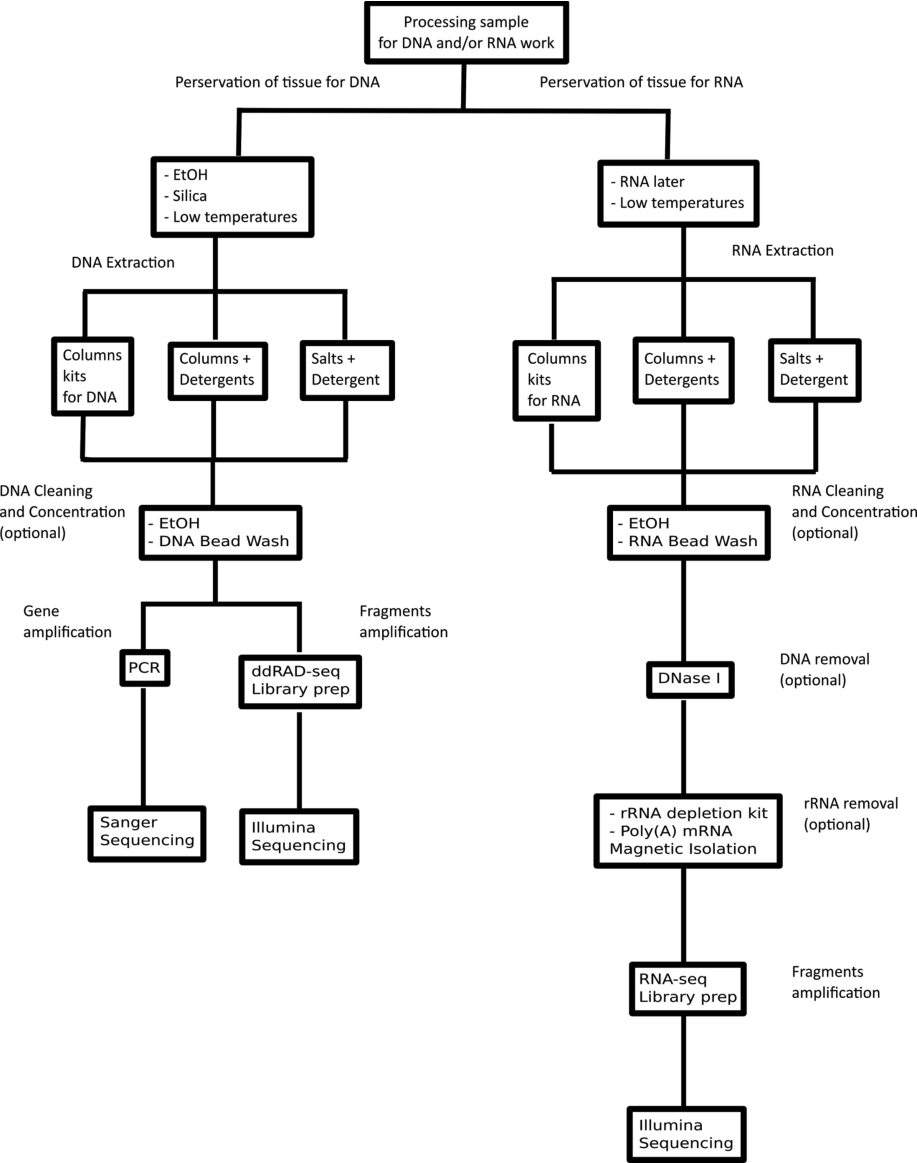
\includegraphics[height=6in]{./images/RNA_DNA_Isolation_Chart.pdf}
		\end{center}
		\end{figure}

	\newpage

	\subsection{Collection of samples for DNA Extraction}

		With next-generation sequencing, we have to try to reduce contamination of our samples with bacteria and other microorganisms, as well as 			from other individuals. Some guidelines:

		\vspace{5mm}

	{\bf Materials}
		
		\begin{itemize}
		\itemsep0em
			\item Scalpels with replaceable, sterile blades
			\item Autoclaved glass pyrex dish for cutting sample on and a flame to torch it; alternatively can use weigh boats that are RNAase/DNAase free
			\item Autoclaved tweezers, probes, etc.  Ideally use tweezers without the ridges, between which tissue gets stuck.
			\item Ethanol in an autoclaved beaker for rinsing dissecting tools
			\item A small flame for sterilizing dissecting tools between samples
			\item Prepared, Autoclaved and labeled (with EtOH-proof pen) microcentrifuge tube(s), filled with 95\% or higher EtOH.  When filling tubes 			do so in a sterile manner (i.e. use a squirt bottle that has been autoclaved or a pipette with autoclaved tips)
		\end{itemize}
	
	{\bf Routine}
		
		\begin{itemize}
		\itemsep0em
			\item Dissect tissue on glass plate and place in microcentrifuge tube
			\item Place the remaining part of the organism in -80$^{\circ}$C and the sample in EtOH in the freezer
			\item Clean glass plate with ethanol and kimwipe, use blade to scrape off any tissue. Ideally flame the glass plate if a torch is available.
			\item Clean dissecting tools in ethanol, use kimwipe if necessary to remove any tissue stuck to them.
			\item Pass dissecting tools over flame
		\end{itemize}

	\newpage
	
	\subsection{Tissue Prep for DNA Extraction}
	
		\begin{enumerate}
			\item {\bf Materials}
			\begin{itemize}
				\itemsep0em
				\item small beaker with DI water
				\item small beaker with EtOH
				\item autoclaved tweezers
				\item weigh boats (enough for each sample)
				\item flame 
				\item lighter
				\item sterile scalpel blades (enough for each sample)
				\item kimwipes
				\item Sterile, labeled microcentrifuge tubes (enough for each sample)
				\item Styrofoam box with ice
				\item Bleach 
				\item 70\% EtOH for cleaning
			\end{itemize}
			
			\item {\bf Procedure}
			\begin{enumerate}
				\item Wash work counter with Bleach first and 70\% EtOH second
				\item Collect 10 samples from freezer and place in ice box. By using only 10 samples at a time, you limit the potential exposure of tissues to temperatures above -20$^{\circ}$C
				\item Place fresh weigh boat on balance and tare it
				\item Remove weigh boat and place first tissue sample into boat
				\item Cut desired amount of tissue using scalpel blade and tweezers and write down final weight in lab notebook
				\item Place tissue into labelled microcentrifuge tube, put directly on ice and put any remaining tissue back into original vial
				\item Throw away scalpel blade in sharps container and throw weigh boat in trash
				\item Clean tweezers:
				\begin{itemize}
					\item Rinse in DI water
					\item Wipe down with a fresh kimwipe
					\item Rinse in EtOH and place directly over flame
				\end{itemize}
				\item Repeat above steps for remaining 9 tissues
				\item Put all 10 original containers and new weighed out samples into -20$^{\circ}$C freezer and collect next 10
				\item Repeat all above steps until all tissues have been prepped
			\end{enumerate}
		\end{enumerate}
			
	\newpage

	\subsection{DNA Isolation Review}

		(adapted from the BITC2441 Lab Manual Fall 2011)

		The fundamental steps of DNA purification are sample lysis and purification of the DNA from contaminants. There are a myriad of protocols 			available for isolating DNA from organisms in the molecular lab. The more classical methods have remained essentially unchanged for decades,		and the more modern methods that involve kits that are commercially available. Basically, the best method for any particular application depends 		on these fundamental considerations: 

		\begin{itemize}
			\itemsep0em
			\item Where the DNA is isolated from will determine the cell lysis techniques used. 
			\item The purity requirements of the intended use of the DNA being isolated will determine how many purification steps will be involved. 
			\item The type of DNA being isolated: genomic DNA has different physical properties from those of plasmid DNA. 
		\end{itemize}

		The successful isolation of DNA requires methods that prevent nuclease degradation of the DNA. Some buffer constituents used to promote lysis 		and denaturation of nucleases include: 

		\begin{itemize}
			\itemsep0em	
			\item Detergents - used to solubilize cell membranes: Popular choices are SDS (sodium dodecyl sulfate, aka SLS, sodium lauryl sulfate), 				Triton X-100, and CTAB (cetyltrimethyl ammonium bromide) 
			\item Proteinase K - sometimes added to cleave glycoproteins and to help the detergents to inactivate DNases. 
			\item Denaturants such as urea, guanidinium salts, and other chaotropes are sometimes applied to inactivate enzymes. Heat is often 				applied to enhance the lysis of cells and the denaturation of proteins. 
			\item For microbial sources of DNA, enzymes must be added to break down cell walls in order to make the cells susceptible to lysis. 
			\item RNases are often added to a lysis buffer to remove contaminating RNAs, which can interfere with the intended use of the DNA being 			isolated. 	
		\end{itemize}

		In selecting a lysis method for a particular application, top priority should be given to choosing a method that has simplicity and speed (least 			number of steps and solutions required). Remember that every constituent added to cells during the lysis procedure could become a culprit by 			sabotaging the activity of an enzyme later on. You will want to remove anything added to your DNA at the beginning of DNA isolation sometime 		later, so try to keep the number of constituents in your lysis buffer to those that are absolutely needed. The number of steps in a cell lysis 				protocol should also be kept to a minimum, since any delays during this part of the DNA isolation procedure runs the risk of DNA degradation by 		nucleases in the cells. DNA will not be safely stabilized until it has been purified from all protein contaminants. In general, animal tissues are 			easily lysed, due to the fact that they have no cell wall, and a gently detergent treatment usually is sufficient to break open cells. Yeast and 			microbial cells, on the other hand, have rigid cell walls that must be weakened enzymatically before the cell will release its DNA. In the case of 			bacteria, lysozyme enzyme is added, while in the case of yeast a more complex mixture of enzymes must be used to degrade cell wall polymers. 		Plant cell walls are generally abraded mechanically by grinding frozen plant tissue, often with glass beads or sand and a mortar and pestle.

		The second phase of DNA isolation protocols is the purification of the DNA released from the cell from other components of the cell and the lysis 		buffer. The method you select for your application depends on the size and source of the DNA to be isolated. When plasmid DNA is being 			isolated from bacteria such as Escherichia coli (E. coli), an alkaline solution of SDS is sufficient to release plasmid DNA, leaving behind the 			genomic DNA still associated with the cellular debris. The genomic DNA is then conveniently removed from the plasmid DNA by a quick 				centrifugation step. Genomic DNA can frequently be rendered insoluble and quickly spooled from the lysed cells by addition of alcohol to the 			mixture. The spooled DNA can be transferred to a fresh buffer to redissolve the genomic DNA.

		For some applications, this low level of DNA purity will suffice. Often, though, there are proteins or polysaccharides (especially in plant sources of 		DNA) that coprecipitate with the DNA and interfere with subsequent enzymatic treatments. Classically, the further purification of DNA involves the 		removal of proteins by aqueous phenol solutions, followed by numerous alcoholic precipitation steps to remove traces of phenol from the isolated 		DNA. Alcohol precipitations of DNA also serve to concentrate the DNA into a smaller volume, and to purify the DNA from any water-soluble 			contaminants. The phenol extraction is an inefficient method of purification and suffers from a poor yield of DNA. Also, phenol reagents are 			unstable, and fresh solutions must be used or the quality of the reagent must be monitored, generally by observed changes in pH. This, along 			with safety concerns in the use of phenolic solutions, is a serious drawback in this method of DNA purification.

		An alternative procedure is the use of so-called spin columns, which are small chromatography columns that purify the DNA from other solutes. 		While this procedure is more expensive than phenol extractions and alcohol precipitations, the purification and yields of product by spin columns 		are improved. Also, the reagents used are more stable, so provide a more reliable, or robust, method. The final DNA prepared with spin columns 		is free of protein and salt contaminants and can be used directly in restriction digests, Southern blotting, and PCR applications. All components 		of this system are stable at room temperature for one year. Another advantage of purchased kits for plasmid preparation is that the quality of 			reagents can be tested and assured the venders. For these reasons, many biotechnology labs routinely use kits for their plasmid preparations.

		Binding and elution from silica beads has become the method of choice for isolation of genomic DNA from animal tissues. A high concentration of 		chaotropes serves to bind nucleic acids to silica surfaces. The adsorption step to bind DNA to the silica particles is followed by wash steps, 			usually with salt/ethanol solutions which will not interfere with the strong binding of nucleic acids but will wash away remaining impurities and 			excess chaotrope. Elution of DNA from silica columns requires the use of nuclease-free water or low ionic strength buffers such as TE. This is an 		advantage since it means that the isolated DNA can be used directly in further manipulations without further cleanup.

		A potential problem with the use of silica columns for the binding of DNA is the possibility of overloading the column with DNA, resulting in a 			wash-through of non-adsorbed DNA and reducing the overall yield of DNA. There is also some loss of material that does not elute from the silica 		resin. The smaller the DNA size is, the tighter is its interaction with silica surfaces. Although size is not a problem with isolations of genomic DNA, 		loading the silica resin with too little DNA can also lead to a low overall yield of DNA eluted from a silica column.

		Protocols for the use of spin columns are unique to each vendor, and so the vendor`s protocol should be followed when they are used. Some 			examples of some more general protocols are found below, along with a discussion of how they work.
		
		NOTE THAT FOR NEXT GENERATION SEQUENCING, SOME METHODS OF DNA EXTRACTION ARE NOT RECOMMENDED.  THIS INCLUDES CTAB EXTRACTION AND PHENOL-CHLOROFORM.

	\newpage 

	\subsection{CTAB DNA Extraction}
		(adapted from Levitan's protocol)
		NOTE THAT FOR NEXT GENERATION SEQUENCING, SOME METHODS OF DNA EXTRACTION ARE NOT RECOMMENDED.  THIS INCLUDES CTAB EXTRACTION AND PHENOL-CHLOROFORM.

		\begin{enumerate}	
		\itemsep0em
			\item Make sure you have all solutions (see solutions sheet for directions). 
			\begin{enumerate}
			\itemsep0em
				\item CTAB
				\item Proteinase K
				\item 100\% Ethanol
			\end{enumerate}
			\item Turn on water bath to begin heating to 65$^{\circ}$C, make sure it has enough water to cover 3/4 of a 1.5 mL microcentrifuge tube. 
			\item Set up and label individual 1.5 mL microcentrifuge tubes.
			\item Add 500 microliters (uL) of CTAB solution to each tube. 
			\item Next add 10 uL of proteinase K solution to each tube, make sure to change tips. If you are processing more than 18 samples at once, 			you should do sets (or stages) of samples so they do not sit for too long. 
			\item Remove a small amount of the sample preserved in EtOH
			\item Blot the sample on kimwipe, and place in microcentrifuge tube. 
			\item Close Tube
			\item Return foreceps to 100\% EtOH to re-sterilize
			\item Repeat steps 4-8 for remaining samples
			\item Place samples in holder (floating) in waterbath. Do not worry too much at this point if the temperature is not quite at 65C
			\item After 30 minutes, mix the samples by inverting gently. 
			\item At this point the temperature should be at 65C, and should be stabilized here.. continue to monitor temperature. 
			\item Leave samples in waterbath overnight (at least 14hours, I have left samples in the waterbath for 48 hours which yielded high DNA 				concentrations). Samples should be digested when you no longer see any gelatinous/stringy material when inverting them.  
			\item Clean your samples by doing a DNA Beadwash (see DNA Beadwash protocol in Appendix)

		\end{enumerate}

	\newpage

\subsection{Cleaning your Sample before DNA extraction- Optional}
This protocol was used for copepod parasites, but could be used for other samples as well.

		\noindent Copepods have a small amount of DNA that can easily be contaminated with other organisms/detritus/plankton/etc present on the 			outside of the body. To avoid contamination, you can add a cleaning step to wash your copepods.

		\begin{enumerate}[leftmargin=.5in]
			\item Prepare small slides of Nylon (6/6) woven mesh sheet (you can cut a 12" width, 12" length, 10 microns mesh size, 2\% open area). Cut 			the mesh to a convenient size that can hold your sample and that will fit in the tube use for digestion with proteinase K. Autoclave the mesh.
			\item Set the mesh and the copepod over an empty clean tube or kimwipe, and add molecular grade ethanol ($<$75\%) to the sample until 			you don`t see any debris or you have given the copepod a few washes. 
			\item Let the copepod dry in a control environment where the copepod won`t fly away (you can set the copepod inside a 1.5 ml 					microcentrifuge tube to dry and use the same tube for the following steps.
		\end{enumerate}

		** Please note that your sample may degrade if you leave it at room temperature for too long. You want to leave your sample to dry for the 			minimum amount of time - avoid overnight drying situations! 

	\newpage

	\titlespacing\subsection{12pt}{12pt}{0pt}
	\subsection{DNA Extraction for Animal Tissues}
		(adapted from DNeasy Blood \& Tissue (cat\#69504) Handbook Introduction)

		\vspace{5mm}
		
		In general, follow the directions supplied with the kit.  \hl{Always cross-check the instructions below with the kit instructions as they may change through time}
	
		{\bf Safety Information}

		\begin{itemize}
		\itemsep0mm
		 	\item When working with chemicals, always wear a suitable lab coat, disposable gloves, and protective goggles. For more information, 				please consult the appropriate material safety data sheets (MSDSs).

			\vspace{3mm}
			{\bf CAUTION: DO NOT} add bleach or acidic solutions directly to sample-preparation waste.
			\vspace{3mm}

			\item Buffer AL and Buffer AW1 contain guanidine hydrochloride, which can form highly reactive compounds when combined with bleach. If 			liquid containing this buffer is spilt, clean with suitable laboratory detergent and water. If the spilt liquid contains potentially infectious agents, 			clean the affected area first with laboratory detergent and water, and then with 1\% (v/v) sodium hypochlorite.
			\item Buffer AL and Buffer AW1 (concentrate) Contains guanidine hydrochloride: harmful, irritant. Risk and safety phrases:* R22- 36/38, 				S13-26-36-46
			\item Proteinase K: sensitizer, irritant. Risk and safety phrases:* R36/37/38-
			42/43, S23-24-26-36/37
		\end{itemize}

		\vspace{5mm}

		{\bf Consumable Supplies and Equipment}

		(Qiagen Kit \#69504 contains all of the reagents except molecular grade ethanol)

		\begin{itemize}
		\itemsep0em
			\item Buffer ATL and Buffer AL. Buffers may form precipitates upon storage. If necessary, warm to 56$^{\circ}$C until the precipitates have 			fully dissolved.
			\item Buffer AW1 and Buffer AW2 are supplied as concentrates. Before using for the first time, add the appropriate amount of ethanol (96-			100\%) as indicated on the bottle to obtain a working solution.
			\item Preheat a thermomixer, shaking water bath, or rocking platform to 56$^{\circ}$C
			\item If using frozen tissue, equilibrate the sample to room temperature. Avoid repeated thawing and freezing of samples since this will lead 			to reduced DNA size.
			\item Vortexer
			\item Molecular grade (100\%) ethanol
			\item Optional: RNase A (100mg/ml; cat. No. 19101)
			\item Microcentrifuges tubes (1.5ml or 2ml) (any type)
			\item Water bath
			\item Centrifuge (that can reach 20000g, room temperature)
			\item Collection tube (provided in the kit)
			\item Columns (provided in the kit)
		\end{itemize}

		\vspace{5mm}

		{\bf Things to do Before Starting}

		Preheat the water bath to 56$^{\circ}$C

		Equilibrate the sample to room temperature
		
		Make sure appropriate rotors are placed in the centrifuge
		
		\vspace{5mm}

		{\bf Protocol}

		\hl{Basically the protocol below is the same as that which comes with the kit.  Some tips: }
		\begin{enumerate}
			\item If the tissue suffered freezer burn, then ice may permeate the tissue and may add to weight.  Suggest thawing small pieces in ethanol to "suck up" water in tissue.
			\item Sterilize blade and tweezers between tissues by rinsing in ethanol, wiping with kimwipe, then rinsing again and burning off ethanol over an open flame. Use a sterilized blade to chop up tissue (stored with dissecting tools below large centrifuge).
			\item If tissue was preserved in ethanol, set up two weigh boats (one on scale).  Pour out tissue and ethanol into weigh boat not on scale.  Blot tissue on kimwipe until completely dry before weighing.  Weigh 25mg.  Take weigh boat off scale and chop tissue.  Store on ice until add buffer ATL and proteinase K.
			\item For tissue digestion lysis step (first step), use Eppendorf thermomixer with 500 rotations per minute.  Also vortex at high speed a few times.
			\item After lysis step and before adding 200ul buffer AL, be sure to vortex for 15 seconds at high speed.
		\item After the protocol below, we elute the DNA in water instead of AE; it might be worse for long-term storage but it should be better for NGS.
		\end{enumerate}
		

		\begin{enumerate}
			\item Use up to 25 mg tissue (up to 10mg spleen). If tissue was preserved in ethanol, then wipe the ethanol of the tissue with kimwipes. Cut up the tissue into small pieces, and place in a 1.5 ml microcentrifuge tube. 
			\item Add 180ul Buffer ATL. 
			\item Add 20ul proteinase K. Mix thoroughly by vortexing, and incubate at 56C until the tissue is completely lysed. Vortex occasionally 				during incubation to disperse the sample. Lysis time varies depending on the type of tissue processed. Lysis is usually complete in 1-3 				hours but if it is more convenient, samples can be lysed overnight; this will not affect them adversely. 
			\item Vortex the lysed sample for 15 seconds. Add 200ul Buffer AL to the sample, and mix thoroughly by vortexing. Then add 200ul molecular grade ethanol 			(100\%), and mix again thoroughly by vortexing. It is essential that the sample, Buffer AL, and ethanol are mixed immediately and 					thoroughly by vortexing or pipetting to yield a homogeneous solution. Buffer AL and ethanol can be premixed and added together in one 				step to save time when processing multiple samples. Some tissues type may form a gelatinous lysate after addition of Buffer AL and 				ethanol. In this case, vigorously shaking or vortexing the preparation is recommended. 
			\item Transfer the mixture from step 4 (including any precipitate) into the the DNeasy Mini spin column placed in a 2ml collection tube. 				Centrifuge at $>$6000 x g for 1 min. Discard flow-through and collection tube. 
			\item Place the DNeasy Mini spin column in a new 2ml collection tube (provided), add 500ul Buffer AW1, and centrifuge for 1 min at $>				$6000 x g. Discard flow-through and collection tube. 
			\item Place the DNeasy Mini spin column in a new 2ml collection tube (provided), add 500ul Buffer AW2, and centrifuge for 3 min at 20000 			x g to dry the DNeasy membrane. Discard flow-through and collection tube. If carryover of ethanol occurs, empty the collection tube, then 			reuse it in another centrifugation for 1 min at 20000 x g. 
			\item Place the DNeasy Mini spin column in a clean 1.5 ml or 2 ml microcentrifuge tube, and pipette 200 ul Buffer AE or water (water is 				advised for ddRAD-seq libraries) directly onto the DNeasy membrane. Incubate at room temperature for 1 min, and then centrifuge for 1 				min at $>$6000 x g to elute. 
			\item Elution with 100ul (instead of 200ul) increases the final DNA concentration in the eluate, but also decreases the overall DNA yield. 
			\item For maximum DNA yield, repeat elution once. A new microcentrifuge tube can be used for the second elution step to prevent dilution 			of the first eluate. 
		\end{enumerate}
	
	
	\newpage



	\subsection{DNA Extraction with QIAamp DNA Micro Kit}

		\begin{center} 
			For purification of genomic DNA from small amounts of tissues or samples (larvae, etc)

			(Adapted from the QIAamp DNA Micro Handbook of Qiagen Cat\# 56304)
		\end{center}

		{\bf Safety Information}

		\begin{itemize}[leftmargin=.5in]
		\itemsep0mm
 			\item When working with chemicals, always wear a suitable lab coat, disposable gloves, and protective goggles. For more information, 				please consult the appropriate material safety data sheets (MSDSs).

			\vspace{3mm}
			{\bf CAUTION: DO NOT} add bleach or acidic solutions directly to sample-preparation waste.
			\vspace{3mm}

			\item Buffer AL and Buffer AW1 contain guanidine hydrochloride, which can form highly reactive compounds when combined with bleach. If 			liquid containing this buffer is spilt, clean with suitable laboratory detergent and water. If the spilt liquid contains potentially infectious agents, 			clean the affected area first with laboratory detergent and water, and then with 1\% (v/v) sodium hypochlorite.
			\item Buffer AL and Buffer AW1 (concentrate) Contains guanidine hydrochloride: harmful, irritant. Risk and safety phrases:* R22- 36/38, 				S13-26-36-46
			\item Proteinase K: sensitizer, irritant. Risk and safety phrases:* R36/37/38-
			42/43, S23-24-26-36/37
		\end{itemize}

		{\bf Consumable Supplies and Equipment}

		(reagents provided with QIAamp DNA Micro Kit (Qiagen \#56304))

		\begin{itemize}[leftmargin=.5in]
		\itemsep0mm
			\item Buffer AL. Check whether precipitate has formed in the buffer. If necessary, dissolve by heating to 70$^{\circ}$C with gentle agitation. 
			\item Buffer AW1. Before using, make sure that 25ml molecular grade ethanol has been added to the bottle; this needs to be done 1 time only. 
			\item Buffer AW2. Before using, make sure that 30ml of molecular grade ethanol has been added to the bottle; this needs to be done 1 time 			only. 
			\item Carrier RNA. Add 310ul Buffer AE to the tube containing 310 ug lyophilized carrier RNA to obtain a solution of 1ug/ul. Dissolve the 				carrier RNA thoroughly, divide it into conveniently sized aliquots, and store at -20$^{\circ}$C. Do not freeze-thaw the aliquots of carrier RNA 			more than 3 times
			\item 1.5 ml microcentrifuge tubes (any kind)
			\item Mesh (optional) - autoclave before use (cat\# CMN-0010-C)
			\item Columns (provided with kit)
		\end{itemize}
		
		\vspace{5mm}
		
		
		{\bf Protocol}

		\begin{enumerate}[leftmargin=.5in]
			\item Transfer a tissue sample of less than 10 mg in weight to a 1.5 ml microcentrifuge tube. If you are working with larvae or small organism, 			dump the sample in a small autoclaved mesh. Then flush the sample with ethanol (the mesh will hold your sample) to get rid of any debris. 			The sample can be transferred with the mesh to the microcentrifuge. 
			\item Immediately add 180 ul Buffer ATL, and equilibrate to room temperature
			(15-25$^{\circ}$C).
			\item Add 20 ul proteinase K and mix by pulse-vortexing for 15 s.
			\item Place the 1.5 ml tube in a thermomixer or heated orbital incubator, and incubate at 56$^{\circ}$C overnight until the sample is completely 			lysed. For small amounts of tissue, lysis is complete in 4-6 h, but best results are achieved after overnight lysis.	
			\item Add 200 ul Buffer AL, close the lid, and mix by pulse-vortexing for 15 s. To ensure efficient lysis, it is essential that the sample and Buffer 			AL are thoroughly mixed to yield a homogenous solution. Note: If you are working with very small samples, add 1ug dissolved carrier RNA to 			the each sample. If working with small larvae, add 8ug dissolved carrier RNA to each sample. 
			\item Add 200 ul ethanol (96-100\%), close the lid, and mix thoroughly by pulse-vortexing for 15 s. Incubate for 5 min at room temperature 			(15-25$^{\circ}$C). Note: If room temperature exceeds 25$^{\circ}$C, cool the ethanol on ice before adding to the tube.
			\item Briefly centrifuge the 1.5 ml tube to remove drops from inside the lid.
			\item Carefully transfer the entire lysate from step 7 to the QIAamp MinElute column (in a 2 ml collection tube) without wetting the rim. Close 			the lid, and centrifuge at 6000 x g (8000 rpm) for 1 min. Place the QIAamp MinElute column in a clean 2 ml collection tube, and discard the 			collection tube containing the flow-through. If the lysate has not completely passed through the membrane after centrifugation, centrifuge 				again at a higher speed until the QIAamp MinElute column is empty.
			\item Carefully open the QIAamp MinElute column and add 500 ul Buffer AW1 without wetting the rim. Close the lid, and centrifuge at 6000 x 			g (8000 rpm) for 1 min. Place the QIAamp MinElute column in a clean 2 ml collection tube, and discard the collection tube containing the flow-			through.
			\item Carefully open the QIAamp MinElute column and add 500 ul Buffer AW2 without wetting the rim. Close the lid, and centrifuge at 6000 x 			g (8000 rpm) for 1 min. Place the QIAamp MinElute column in a clean 2 ml collection tube, and discard the collection tube containing the flow-			through. Contact between the QIAamp MinElute column and the flow-through should be avoided. Some centrifuge rotors may vibrate upon 			deceleration, resulting in the flow-through, which contains ethanol, coming into contact with the QIAamp MinElute column. Take care when 			removing the QIAamp MinElute column and collection tube from the rotor, so that flow-through does not come into contact with the QIAamp 			MinElute column.
			\item Centrifuge at full speed (20,000 x g; 14,000 rpm) for 3 min to dry the membrane completely. This step is necessary, since ethanol 				carryover into the eluate may interfere with some downstream applications.
			\item Place the QIAamp MinElute column in a clean 1.5 ml microcentrifuge tube and discard the collection tube containing the flow-through. 			Carefully open the lid of the QIAamp MinElute column and apply 20=100 ul Buffer AE or distilled water to the center of the membrane. If high 			pH or EDTA affects sensitive downstream applications, use water for elution. Important: Ensure that Buffer AE or distilled water is equilibrated 			to room temperature (15-25$^{\circ}$C). If using small elution volumes ($<$50 ul), dispense Buffer AE or distilled water onto the center of the 			membrane to ensure complete elution of bound DNA. QIAamp MinElute columns provide flexibility in the choice of elution volume. Choose a 			volume according to the requirements of the downstream application. Remember that the volume of eluate will be up to 5 ul less than the 				volume of the solution applied to the column.
			\item Close the lid and incubate at room temperature (15-25$^{\circ}$C) for 1 min. Centrifuge at
			full speed (20,000 x g; 14,000 rpm) for 1 min. Incubating the QIAamp MinElute column loaded with Buffer AE or water for 5 - 30 min at room 			temperature before centrifugation generally increases DNA yield.
		\end{enumerate}
	
	\newpage

	\subsection{RNA Isolation Review}

		(adapted from the BITC2441 Lab Manual Fall 2011 and Vomelova et al. 2009)

		\vspace{3mm}
		
		\noindent RNA may be used in the molecular lab to make cDNA in order to clone genes, to study gene regulation, to determine the size and 			structure of specific messages, the identify gene products, to determine rates of specific mRNA synthesis or degradation, to name a few. There are 		many procedures for isolating RNA, depending on the type of RNA to be isolated, the type of tissue that the RNA is being isolated from, and the 		intended use of the isolated RNA. The successful isolation of intact RNA by any procedure requires that four important steps be performed: 
		
		\begin{enumerate}
			\itemsep0mm
			\item effective disruption of cells or tissue 
			\item denaturation of nucleoprotein complexes 
			\item inactivation of endogenous ribonuclease (RNase) activity 
			\item purification of RNA away from contaminating DNA and protein 
		\end{enumerate}


		\noindent The most important of these is the immediate inactivation of endogenous RNase activity which is released from membrane-bound 			organelles upon cell disruption. RNases are very stable and generally require no cofactors such as magnesium and other divalent cations, so they 		cannot be 	inhibited or inactivated by adding chelators such as EDTA.
		
		\vspace{3mm}
		
		\noindent Tissues to be used for the isolation of RNA should be properly stored immediately after collection to prevent RNA degradation from the 		activity of RNases. To do so, the tissue should be preserved under -70 C temperatures (flash freezing with liquid nitrogen preferred) or the tissues 		should be 	preserved in a preservative agent that inactivates RNases (such as RNA later). The quality of the RNA to be isolated would depend 			greatly in reducing the amount of elapse time from killing an organism and preserving the tissue. 
		
		\vspace{3mm}

		\noindent Prior to the isolation of RNA, the tissues have to go through an enzymatic or mechanical process. Potent RNase inactivating ingredients 		that denature proteins (including RNases) are added to the lysing buffer. The most effective and most commonly used denaturant is guanidinium 		isothiocyanate (usually abbreviated as GITC or GuSCN). Another strong protein denaturant is phenol (which is also very caustic!), and historically, 		phenol or mixtures of phenol and chloroform were used in RNA isolation. Detergents are also able to denature proteins and most lysis solutions 		contain detergents. These denaturing agents also disrupt cell membranes and aid in solubilization of the tissue.
		
		\vspace{3mm}
		
		\noindent RNA isolation methods fall in three approaches 1) procedures relying on the different solubility of cellular components in organic solvents, 		such as phenol, ethanol or isopropanol; 2) methods based on RNA adsorption to specific surfaces in the presence of chaotropic salts; and 3) 			protocols exploiting RNA separation on isopycnic gradient centrifugation. 
		
		\vspace{3mm}
		
		\noindent The choice of an RNA isolation method depends upon a number of factors, such as: 
		
		\begin{enumerate}
			\itemsep0mm
			\item the source of RNA - i.e., tissues with high fat content have different isolation requirements 
			\item the type of RNA to be purified 
			\item the relative abundance of the RNA 
			\item the sample size 
		\end{enumerate}

		\noindent Once RNA has been isolated, it is usually resuspended in water or water with trace amount of salts or EDTA. At this point the RNA is 		unprotected and highly vulnerable to degradation. Therefore it is extremely important that surfaces and solutions, which come into contact with the 		RNA 	preparation, are completely free of active RNase. 
		
		\vspace{3mm}
		
		\noindent Because of the stringent requirements for high-quality reagents, many if not most labs prefer to purchase RNA isolation kits from 			commercial sources where the quality of the materials have been validated and spin columns help to speed the extraction process.

		\vspace{3mm}
		
		\noindent{\bf TECHNIQUE TIPS: }

		\begin{enumerate}
			\itemsep0mm
			\item Observe all the guidelines for creating an RNase-free working environment in your workspace and lab. 
			\item Keep reagent bottles closed if not in use. 
			\item Keep tissues, reagents, and RNA samples on ice to prevent degradation by RNases.  
		\end{enumerate}
		
		\newpage

	\subsection{Creating a RNase-FREE Environment}
	
		(adapted from the BITC2441 Lab Manual Fall 2011 and Vomelova et al. 2009)
	
		\vspace{3mm}
	
		\noindent RNases are ubiquitous and notoriously difficult to inactivate. The following notes are good things to consider in setting up for an RNA 		isolation: 
		
		\begin{enumerate}
		
			\item Two of the most common sources of RNase contamination are the researcher`s hands and bacteria or molds that may be present on 			airborne dust particles or laboratory equipment and supplies. To prevent contamination from these sources, sterile technique should be 				employed when handling any of the reagents used for RNA isolation or analysis. Gloves should be worn at all times and exchanged often.  

			\item To avoid RNA degradation, all solutions, glassware, and plasticware that may contain RNase should be treated to remove RNases. 				Diethylpyrocarbonate (DEPC) inactivates RNases by reacting with histidine residues, found at the active site and so is the usual method for 			producing RNase-free equipment. To render water RNase-free, it is treated as follows: 
				
			\begin{itemize}
				\itemsep0em
				\item Measure water into RNase-free glass bottles. 
				\item Add diethylpyrocarbonate (DEPC) to make a 0.1\% (v/v) solution. (ie add 0.1 mL  DEPC for each 100 mL of water). 
				\item Shake vigorously to mix 
				\item Autoclave for 15 minutes at 121o C on liquid cycle, OR incubate at least 12 hours at 37$^{\sim}$C and then heat to 100$^{\sim}$C 				for 15 minutes. 
			\end{itemize}
				
			\noindent {\bf NOTE:} Tris buffers cannot be treated with DEPC. DEPC is a suspected carcinogen and should be handled with care. Always 			use gloves and open under a fume hood. 

			\item Disposable plasticware such as pipette tips and microcentrifuge tubes is generally RNase free if used straight out of the package and 			the package is kept closed and gloves are worn when items are touched and removed. It is best to pour tubes from an unopened bag onto an 			RNase-free environment (such as plastic wrap). 

			\item Chemicals and equipment for use in RNA isolation and analysis would be best reserved separately from other uses. Wear gloves when 			handling this equipment, and use only baked spatulas and untouched weigh boats or weigh paper. 

			\item Use filter-tips for micropipetting when isolated RNA is to be used in amplification procedures. 

			\item Use heat-blocks and not water baths. Dirty water baths are a source of RNases. 

			\item Clean counter with bleach, EtOH, and RNAase away. Once the surface is clean, don't put anything on it that hasn't been treated.  Make sure if you move something to another counter and move it back, to treat the bottom.
			
			\item After extraction, RNA can be stored in RNA-ase free TE or RNA-ase free 1mM EDTA.
			
			\item There are guidelines online for RNAase free plasticware.

 		\end{enumerate}
			
		\newpage

	\subsection{Qiagen RNA extraction} 
	
		\noindent (adapted from RNeasy Mini Kit Handbook, RNeasy Plus Universal Handbook and Fuxjager Lab)
	
		\vspace{5mm}

		\noindent For purification of total RNA from animal tissues. RNeasy Mini Kit Protocol (Qiagen \#73404). RNeasy Plus University Mini Kit combines 		the use of Qiazol with the kit - we should probably switch to this kit (Qiagen \#73404). 
	
		\vspace{5mm}
		
		\noindent {\bf Introduction}

		\noindent This kit purifies all RNA molecules longer than 200 nucleotides from up to 50 mg of tissue (or up to 100 mg of brain or adipose tissue) per 		RNeasy Mini spin column. 
		
		\vspace{5mm}
		
		\noindent {\bf Safety Information}
		
		\vspace{3mm}
		
		\begin{adjustwidth}{0.5in}{0pt} {\bf CAUTION: DO NOT add bleach or acidic solutions directly to the sample-preparation waste}
		\end{adjustwidth}
		
		\vspace{3mm}
		
		\noindent Trizol Lysis Reagent and Buffer RW1 contain guanidine thiocyanate. Guanidine salts can form highly reactive compounds when 			combined with bleach. If liquid containing these buffers is spilt, clean with suitable laboratory detergent and water.
		
		\vspace{3mm}
		
		\noindent Use a double pair of nitrile gloves when handling Trizol. 
		
		\vspace{3mm}
		
		\noindent The solid waste of anything that touches the bugger and/ or reagents of the RNeasy Mini Kit, Trizol, or chloroform should be discarded in 		the Organic Solvent Carboy, and the solids that touch these solutions should be discarded in the Research Solid Waste.
 
		\vspace{5mm}
		
		\noindent {\bf Consumable supplies}
		
		\begin{itemize}
			\itemsep0em
			\item RNeasy Mini Kit (Qiagen \#74104)		
			\item 1.5 microcentrifuges tubes (4 per sample)	
			\item Culture test tubes (1 per sample plus 4 tubes for washing) 
			\item 75\% ethanol (to clean counter) 
			\item RNase Away (VWR \#72830-022)
			\item Bleach
			\item Kimwipes 
			\item Chloroform (try to use chloroform without ethanol if possible)
			\item Trizol
			\item 70\% ethanol (molecular grade and made with DEPC treated water)
			\item DEPC treated water
			\item Nitrile Gloves (why Nitrile) (Use of Trizol and Phenol which are highly toxic and corrosive requires a thicker, more durable glove than 			latex) 
 		\end{itemize}

		\noindent {\bf Equipment}
			
			\begin{itemize}
				\itemsep0mm
				\item Tissue homogenizer (9001271) (alternative homogenizer with exchangeable probes (probes Cat\#02-070-MGXL-12) (homogenizer 				- any PRO homogenizer model from pro scientific). 
				\item Centrifuge 5430 R (Eppendorf)
			\end{itemize}
		
		\vspace{5mm}
		
		\noindent {\bf Things to do before}
				
			\begin{itemize}
				\itemsep0em
				\item[--] Make sure RPE buffer has 4 volumes of ethanol (100\%)
				\item[--] Prepare your 70\% diluted ethanol with DEPC treated water
				\item[--] Set centrifuge to 4$^{\sim}$C
				\item[--] Label 4 microcentrifuge tubes per sample (1 will be used for the final storage of RNA, and 1 for the working stock to use for 					quantity and quality assessment)
				\item[--] Label 1 RNeasy Mini spin column per sample
				\item[--] Get one 2ml additional collection tube per sample from the RNA kit. 
				\item[--] Clean your working area (hood) and supplies with Bleach, then Ethanol (75\%), then RNase Away, then Ethanol (75\%)
				\item[--] Wash the homogenizer with Trizol (*Trizol source should be kept in ice or put back in the 4C refrigerator when not in use). 
				\item[--] Label a culture tube for each of the four steps needed to clean the homogenizer (2 water steps, 1 ethanol step and 1 Trizol 					step). 
				\item[--] Get ice (to transfer reagents and RNA) (ice code is 6907)
			\end{itemize}
				
			\vspace{3mm}
			
		{\bf Protocol}
			
		\noindent *these steps are to be done in the hood unless noted otherwise
	
		\begin{enumerate}
			\itemsep0em
			\item Sterilize your tools for handling tissue and minimizing contamination among samples **This step and the weighing of the tissue can 				be done outside the hood
			\item Add 1ml volume of Trizol Lysis reagent to the culture test tubes (prepare a tube per sample and one additional trizol tube for washing)
			\item ***Gloves: If accidental contact occurs, remove and discard contaminated gloves immediately (The breakthrough time for a 4 mm 				nitrile glove is approximately 3 minutes for chloroform)
			\item * Put the Trizol back on ice or in the 4C refrigerator
			\item Add 1ml volume of DEPC treated water to two culture tubes for washing the homogenizer (be sure to label tubes to not confuse with 			ethanol wash tube)
			\item Add 1ml volume of 70\% ethanol molecular grade to a culture tube for washing the homogenizer
			\item Clean homogenizer before the first sample and between each homogenization of the samples following these steps:
				
				\begin{itemize}
					\itemsep0em 
					\item clean the probe with a tissue and rinse in sterile DEPC treated water
					\item dry the probe with a tissue and rinse in 70\% ethanol (molecular grade and made with DEPC treated water)
					\item dry the probe with a tissue and rinse in sterile DEPC treated water
					\item dry the probe with a tissue and rinse in trizol 
				\end{itemize}
				
			\item Get your samples out from the -20 (once you have everything set up and ready to work with the samples)
			\item Weigh and transfer your tissue to a culture tube with Trizol for homogenization: 100 mg of brain tissue, 30 mg of adipose, liver, spleen, 			or thymus tissue, or 50mg tissue for other tissues
			\item * When weighing tissue stabilized in RNAlater,  remove any crystals that may have formed (with sterilized forceps)
			\item * Tissues not treated with RNAlater should not be allowed to thaw and the tissue should be cut into smaller parts in dry ice 
			\item Homogenize the lysate using the Tissue Rupture for 20-40 seconds depending on the toughness and size of the sample
			\item Place the tip of the probe half the distance from the bottom of the tube and against the side of the tube. This will minimize foaming. 				Half the speed will sufficiently disrupt the tissue without producing foam
			\item When homogenization is complete, decrease the speed of the probe to low and gently tap the probe against the side of the tube and 			remove from the solution in order to minimize the amount of sample remaining in the probe
			\item Wash homogenizer between samples using the steps explained above
			\item * Foaming may occur during homogenization. Let the homogenate stand at room temperature for 2-3 min until the foam subsides before 			continuing with the procedure
			\item Transfer the lysate to a labeled 1.5 mL epi tube
			\item Place the tube containing the homogenate on the benchtop at room temperature (15-25C) for 5 min
			\item Change your gloves
			\item Add 200 ul chloroform (use chloroform without ethanol if available). Securely cap the tube containing the homogenate, and shake it 				vigorously for 15s
			\item Place the tube containing the homogenate on the benchtop at room temperature for 2-3min
			\item Centrifuge at 13,000 x g for 15 min at 4C
			\item After centrifugation, the sample separates into 3 phases: an upper, colorless, aqueous phase containing RNA; a white interphase; and a 			lower, red, organic phase. For tissues with an especially high fat content, an additional, clear phase may be visible below the red, organic 			phase. The volume of the aqueous phase should be approximately 600 uL
			\item After centrifugation, heat the centrifuge to room temperature (15-25C) 
			\item To warm up the Centrifuge 5430R, set the centrifuge to 25C and press the fast button
			\item Transfer $\sim$80\% of the upper aqueous phase to a new 1.5 mL epi-tube, be careful not to take any of the middle phase
			\item With a 200ul pipette, remove 200ul at a time. Ideally, only remove 400ul total from the upper aqueous phase 
			\item Discard the middle and bottom phase
			\item Add 1 volume (usually 400-500 ul) of 70\% ethanol to the recovered aqueous phase, and mix thoroughly by pipetting up and down
			\item Precipitates may be visible after addition of ethanol. Resuspend precipitates completely by vigorous shaking, and proceed immediately 			to step 
			\item Transfer up to 700 ul of the sample to an RNeasy Mini spin column placed in a 2ml collection tube. Close the lid gently, and centrifuge 			for 15s at 13000 x g at room temperature (15-25C). Discard the flow-through. Repeat the step with any remainder of the sample using the 			same collection tube
			\item Add 700 ul Buffer RW1 to the RNeasy spin column. Close the lid gently, and centrifuge for 15s at 13000 x g to wash the membrane. 			Discard the flow-through. Reuse the collection tube in the next step
			\item After centrifugation, carefully remove the RNeasy spin column from the collection tube so that the column does not contact the flow-				through. Be sure to empty the collection tube completely
			\item Add 500 ul Buffer RPE to the RNeasy spin column. Close the lid gently, and centrifuge for 15s at 13000 x g to wash the membrane. 				Discard the flow through. Reuse the collection tube for the next step
			\item Add 500 ul Buffer RPE to the RNeasy spin column. Close the lid gently, and centrifuge for 2 min at 13000 x g to wash the membrane. 			Discard the flow through
			\item After centrifugation, carefully remove the RNeasy spin column from the collection tube so that the column does not contact the flow-				through. Otherwise, carryover of ethanol will occur
			\item Place the RNeasy spin column in a new 2ml collection tube, and discard the old collection tube with the flow-through. Close the lid 				gently, and centrifuge at 18000 x g for 1 min (to remove carryover of Buffer RPE)
			\item Place the RNeasy spin column in a new labeled 1.5ml epi tube. Add 30-50 ul RNase-free water directly to the spin column membrane. 			Close the lid gently. To elute the RNA, centrifuge for 2:30 min at 13000 x g
			\item * for higher RNA recovery, incubate the RNeasy spin column on the benchstop for 1-2 min with RNase-free water before centrifuging.
			\item Place the recovered RNA on ice right away and then transfer to the -20
			\item Repeat the above step using another volume of RNase-free water, or using the eluate from step 15 (if high RNA concentration is 				required). Reuse the collection tube from prior step
			
			** reusing the eluate will be 15-30\% less than that obtained using a second volume of RNase-free water, but the final RNA concentration 				will be higher
			
			\item Place the recovered RNA on ice
			\item Transfer 5 uL of eluted RNA into second 1.5 mL epi tube as a working stock: 1 uL will be used for Nanodrop quality assessment, 1 uL 			will be used for Qubit quality assessment, 2 uL will be used for Agarose gel quality assessment
		\end{enumerate}
			
		{\bf**Make note of phenol solving problem in black rockfish breakdown}
		
	\newpage
		
		
	\subsection{DNA-Free RNA Kit}
		
		\noindent (Now Called RNA Clean \& Concentrator-5 from Zymo Research)
		
		\vspace{3mm}
		
		\noindent Cleans up to $\sim$5ug of RNA product from DNA and some impurities. Although the last RNeasy Mini Kit contains some DNAase1, 			most protocols recommend doing an additional cleaning step with the DNA-Free RNA Kit. 
		
		\vspace{5mm}
		
		{\bf Consumable supplies}
		
		\begin{itemize}
			\item RNA Clean \& Concentrator -5 Kit (Zymo Research \#R1013)
			\item 100\% molecular grade ethanol
			\item 1.5 mL epi tubes (3 per sample)
		\end{itemize}
		
		\vspace{3mm}
		
		{\bf Things to do before}
			
		\begin{itemize}
			\item[--] Make sure the RNA wash buffer has the appropriate amount of ethanol added.
			\item[--] If using a new kit before starting, add 48 ml 100\% ethanol (52 ml 95\% ethanol) to the 12 ml RNA Wash. Buffer concentrate (R1013) 			or 96 ml 100\% ethanol (104 ml 95\% ethanol) to the 24 ml RNA Wash Buffer concentrate (R1014).
			\item[--] Label 3 RNase-free 1.5 mL epi tubes per sample.
			\item[--]  1 epi tube to be used to transfer the amount of RNA needed for the DNase I mix.
			\item[--] 1 epi tube to be used for the elution of your RNA.
			\item[--] 1 epi tube to be used as a working stock of your eluted RNA for quality. and quantity assessment.
			\item[--] Label 1 column collection tube per sample
			\item[--] Bring 100\% molecular grade ethanol.
			\item[--] *** Follow RNA working procedures to assure the procedure is performed in an RNase-free envornoment (work in the hood, clean 			everything well, keep your samples in ice - when they are not in columns, etc).
			\item[--] *** Some of the reagent contains Chaotropic reagents. Irritant. Please discard the waste of this procedure appropriately and use 				proper safety precautions with the reagents. 
		\end{itemize}
		
		\vspace{3mm}
		
		{\bf Protocol}
		
		\noindent (for small RNA elimination for total RNA of $>$ 200 nt)
	
		\vspace{3mm}
		
		\noindent ** Please look at the original protocol from Zymo if you want to get RNA smaller than 200 nt.
		
		\begin{enumerate}
			\item Digest RNA samples with DNase I.
			\begin{itemize}
				\item[--] Transfer 20 ul of RNA sample (($<$5ug) in water or TE Buffer) to a 1.5 mL epi tube
				\item[--] Add the following mix to each sample RNA sample:
			\end{itemize}
				
			\begin{table}[h]
				\centering
				\begin{tabular}{| c | >{\centering\arraybackslash}m{10em} |}
				\hline
				\cellcolor{gray}{\bf Reagent} & \cellcolor{gray}{\bf Number of samples 1X (uL)}  \\
				\hline
				10x DNase I Buffer & 5 uL \\
				RNase-Free DNase I & 2 uL \\
				RNase-Free Water & 23 uL \\
				\hline
				\end{tabular}
			\end{table}

			\item Mix 1 volume of RNA Binding Buffer with 1 volume ethanol (95-100\%) (e.g., 50 ul buffer and 50 ul ethanol).
			\item Add 2 volumes of the adjusted buffer from step 2 to 1 volume of RNA sample mix from step 1 (e.g., 100 ul adjusted buffer and 50 ul 				sample) and mix well.
			\item Transfer the mixture to the Zymo-Spin IC Column in a Collection Tube and centrifuge at $\geq$12,000 x g for 1 minute. Discard the flow-			through.
			\item Add 400 ul RNA Prep Buffer to the column and centrifuge at $\geq$12,000 x g for 1 minute. Discard the flow-through.
			\item Add 800 ul RNA Wash Buffer to the column and centrifuge at $\geq$12,000 x g for 30 seconds. Discard the flow-through. Repeat the 			wash step with 400 ul RNA Wash Buffer.
			\item Centrifuge the Zymo-Spin IC Column in an emptied Collection Tube at $\geq$12,000 x g for 2 minutes. Remove the Zymo-Spin IC 					Column carefully from the Collection Tube and transfer it into an epi tube.
			\item Add $\geq$6 ul of DNase/RNase-Free Water directly to the column matrix and let stand for 1 minute at room temperature. Centrifuge at 				10,000 x g for 30 seconds. The eluted RNA can be used immediately or stored at -70$^{\circ}$C. 
				\begin{adjustwidth}{0.75in}{0pt}** Waiting for 1 to 2 minutes after adding the RNase-free water to the column matrix may increase RNA 				yield. Also, the yield may be increased by performing a second elution.
				\end{adjustwidth}
			\item Remove 5 ul of the RNA, if you have enough RNA for your work, and transfer it to a new 1.5 mL epi tube to be used for your quality and 			quantity assessments (this will protect your original RNA from thawing and additional exposure to the environment). 
				\begin{itemize}	
					\item[--] 1 uL will be used for Nanodrop quality/quantity assessment
					\item[--] 1 uL will be used for Qubit quality/quantity assessment
					\item[--] 2 uL will be used for Agarose gel quality assessment
				\end{itemize}
		\end{enumerate}
			
	\newpage
			
\section{ddRAD-seq}
	Amplified restriction fragments for genomic enrichment
\hl{NOTE THIS SECTION IS UNDER CONSTRUCTION}
		\vspace{5mm}

	\subsection {DNA Extraction}

		\begin{adjustwidth}{0.5in}{0pt} Follow instructions for Qiagen DNA Blood \& Tissue Kit (page 28).  We don`t use RNA removal, although if we 			were going to do it we would add RNase A (cat \# 19101) while extracting the DNA with the Qiagen DNA Blood \& Tissue Kit. At the end of the extraction, store the DNA in autoclaved Milli-Q water.  
		
		\hl{Should we recommend beadwash after DNA Extraction?}
		\end{adjustwidth}

\subsection {Overview of ddRAD Protocol}

		\begin{adjustwidth}{0.5in}{0pt} Genomic DNA is first digested with two restriction enzymes. This results in a pool of fragments that have the sticky-		ended restriction cut sites on either end, and these ends provide a template for ligation of the customized adaptor sequences. The adaptor 			sequences contain the Illumina adaptors and primer sequences for multiplexing sequencing (and hence provide a binding site for the Illumina PCR 		primers), and the first barcodes of 5-8 base pairs are incorporated to the left adaptor. The bases at one of the end of each adaptor oligo correspond to the ligation site; that is, they match the restriction cut site.  NOTE THAT WE MAKE SURE OUR BARCODE DESIGN DOES NOT RE-CREATE THE RESTRICTION SITE.  This can be important when using MspI, which is not inactivated by heat. The ligation reaction is pooled and concentrated with a bead wash in preparation for the size selection step. Size selection allows the fragments that are too small or oversized to be removed. The fragments of the appropriate size are 	amplified through a Polymerase Chain Reaction where the fragments with the left and right adapters get amplified (fragments that carry the wrong combination of adapters won`t amplify due to the selectiveness of the right adapter). The amplified products now have 2 barcodes, and they can be pooled and concentrated with a bead wash. The final library is good for paired-end sequencing. 
		
		In January 2016 we ordered new adapters and made some modifications.  The first modification was to use the Peterson protocol, instead of a mix of different protocols.  The second modification was the adapters.  Both the p5 and p7 adapters were designed to be offset by a 0-2 bp insertion.  For both reads, this will offset the sequencer at the restriction site so that it is not blinded by the laser. The p7 adapter (right) was designed to also contain a 4-bp degenerate base sequence that we can use to identify PCR duplicates.  This sequence was accompanied by another 4-bp that were designed to making sure the adapters anneal together well.
		
		FOR DDRAD, YOU SHOULD CHOOSE ENZYMES THAT ARE NOT SENSITIVE TO DNA METHYLATION.
		
		\end{adjustwidth}

		\begin{figure}[h]
			\hspace*{-0.75in}
			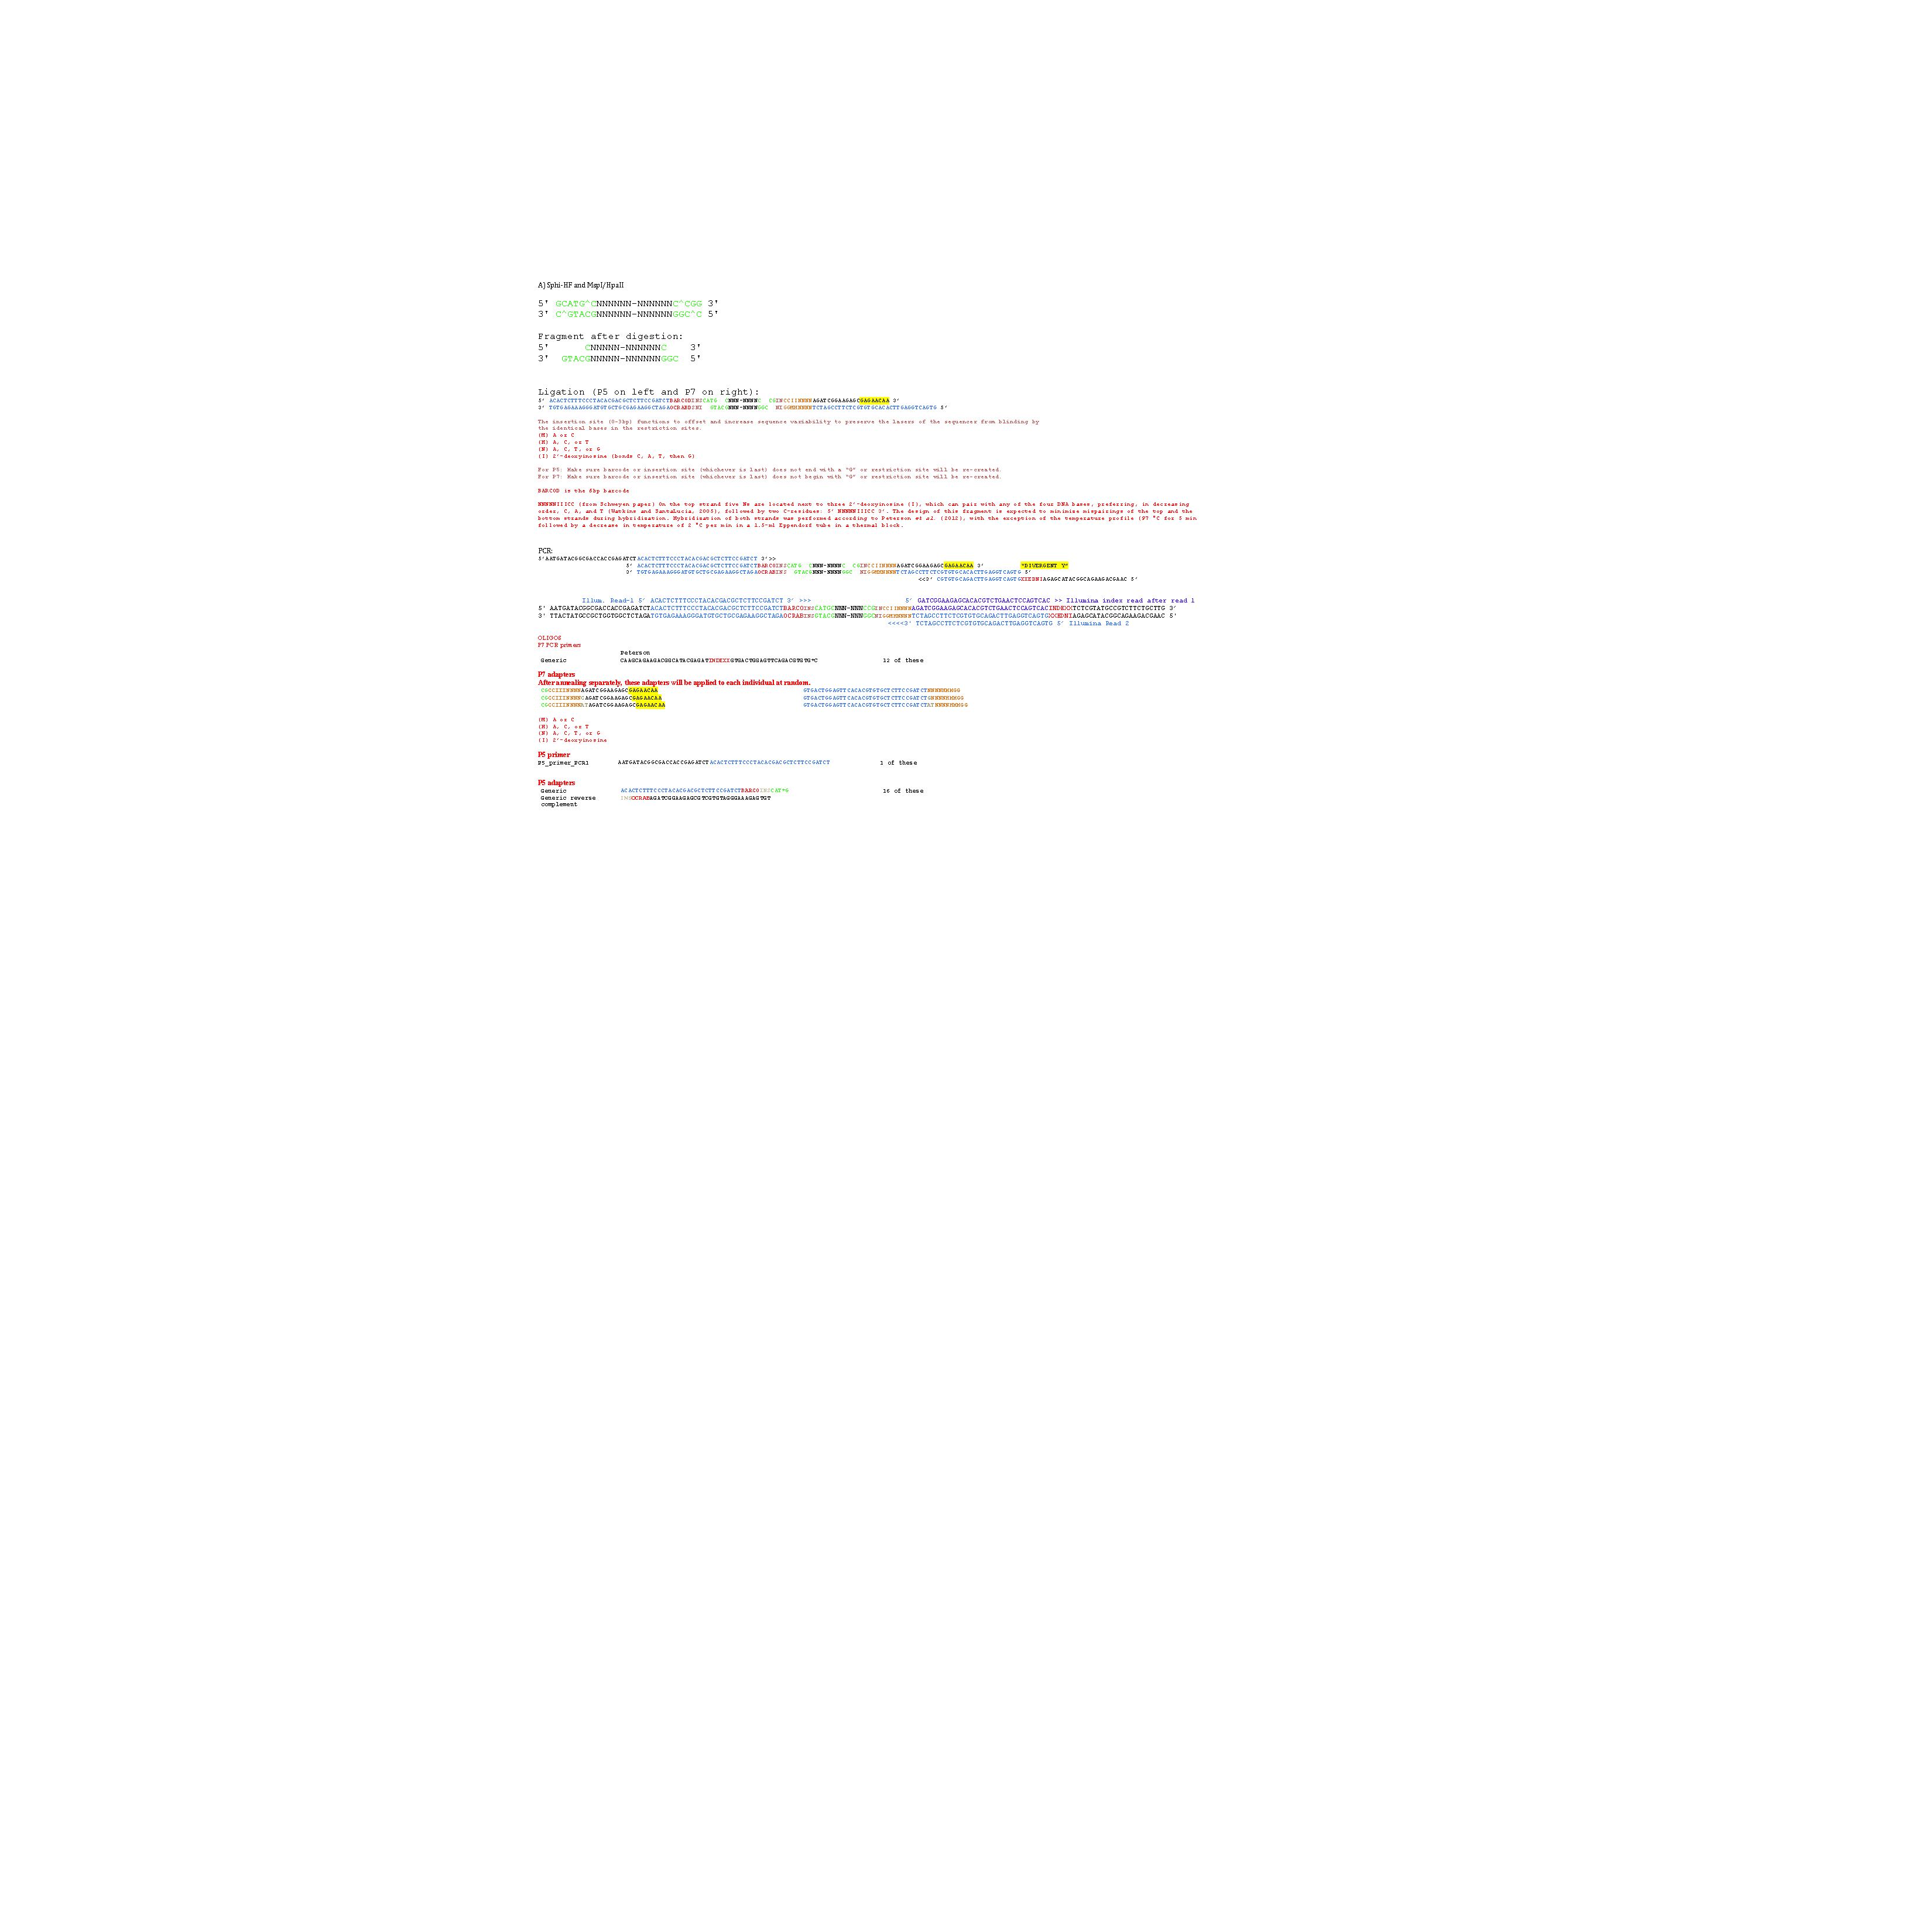
\includegraphics[width = 8in]{./images/20160109_ddRAD_methylRAD_Lotterhos_design.pdf}
			\caption{ddRAD and methylRAD adapter design}
		\end{figure}

		\vspace{5mm}
	\clearpage
	\newpage 
	
	\subsection {Overview of methylRAD Protocol}
		The methylRAD protocol follows the ddRAD protocol, except first the DNA from each individual is split in half.  Each half is digested with a pair of restriction enzymes: R1-MspI or R1-HpaII.  HpaII will not cut at a methylated site, so we predict that we can compare the proportion of reads at the cutsite to infer whether that site is methylated.  Here is the conceptual idea:
		\begin{figure}[h]
			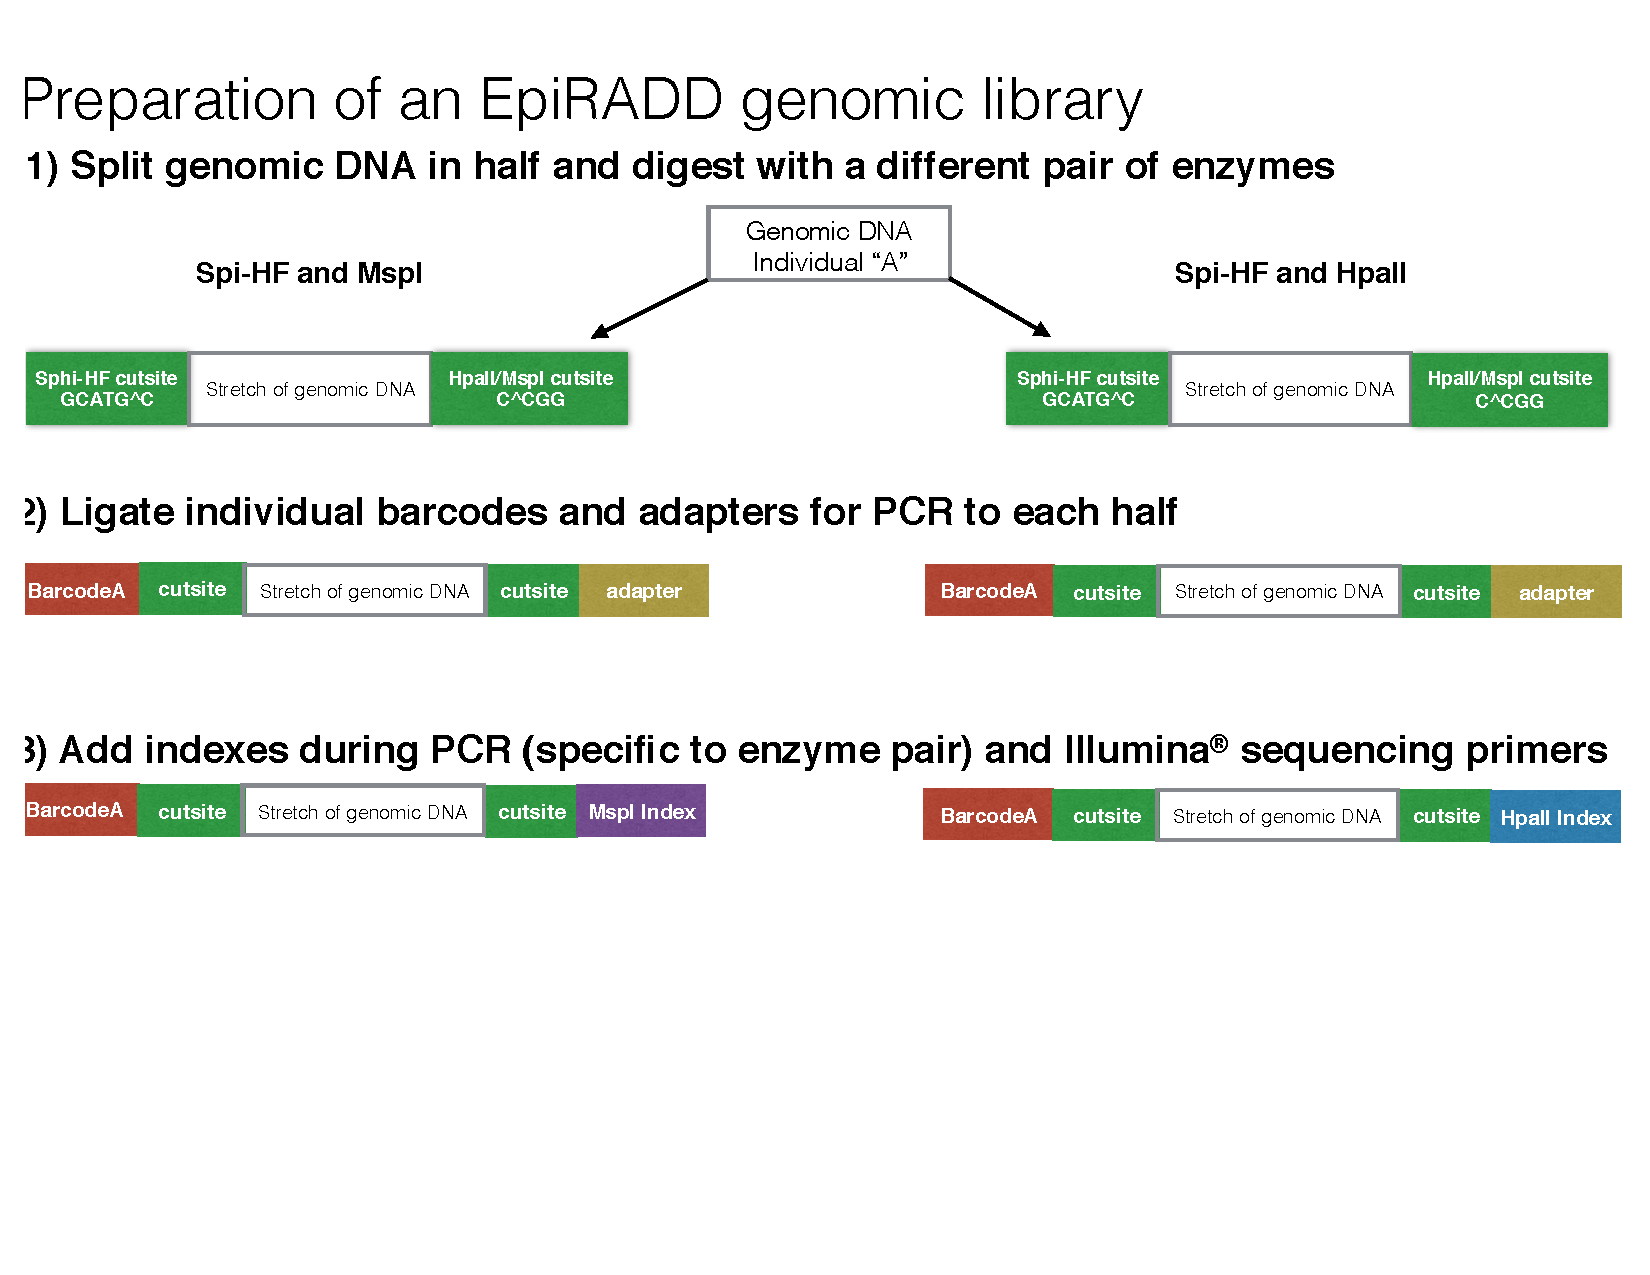
\includegraphics[width=5in]{./images/methylRAdd_prep.pdf}
			\caption{Overview of methylRAD library prep}
		\end{figure}
		\begin{figure}[h]
			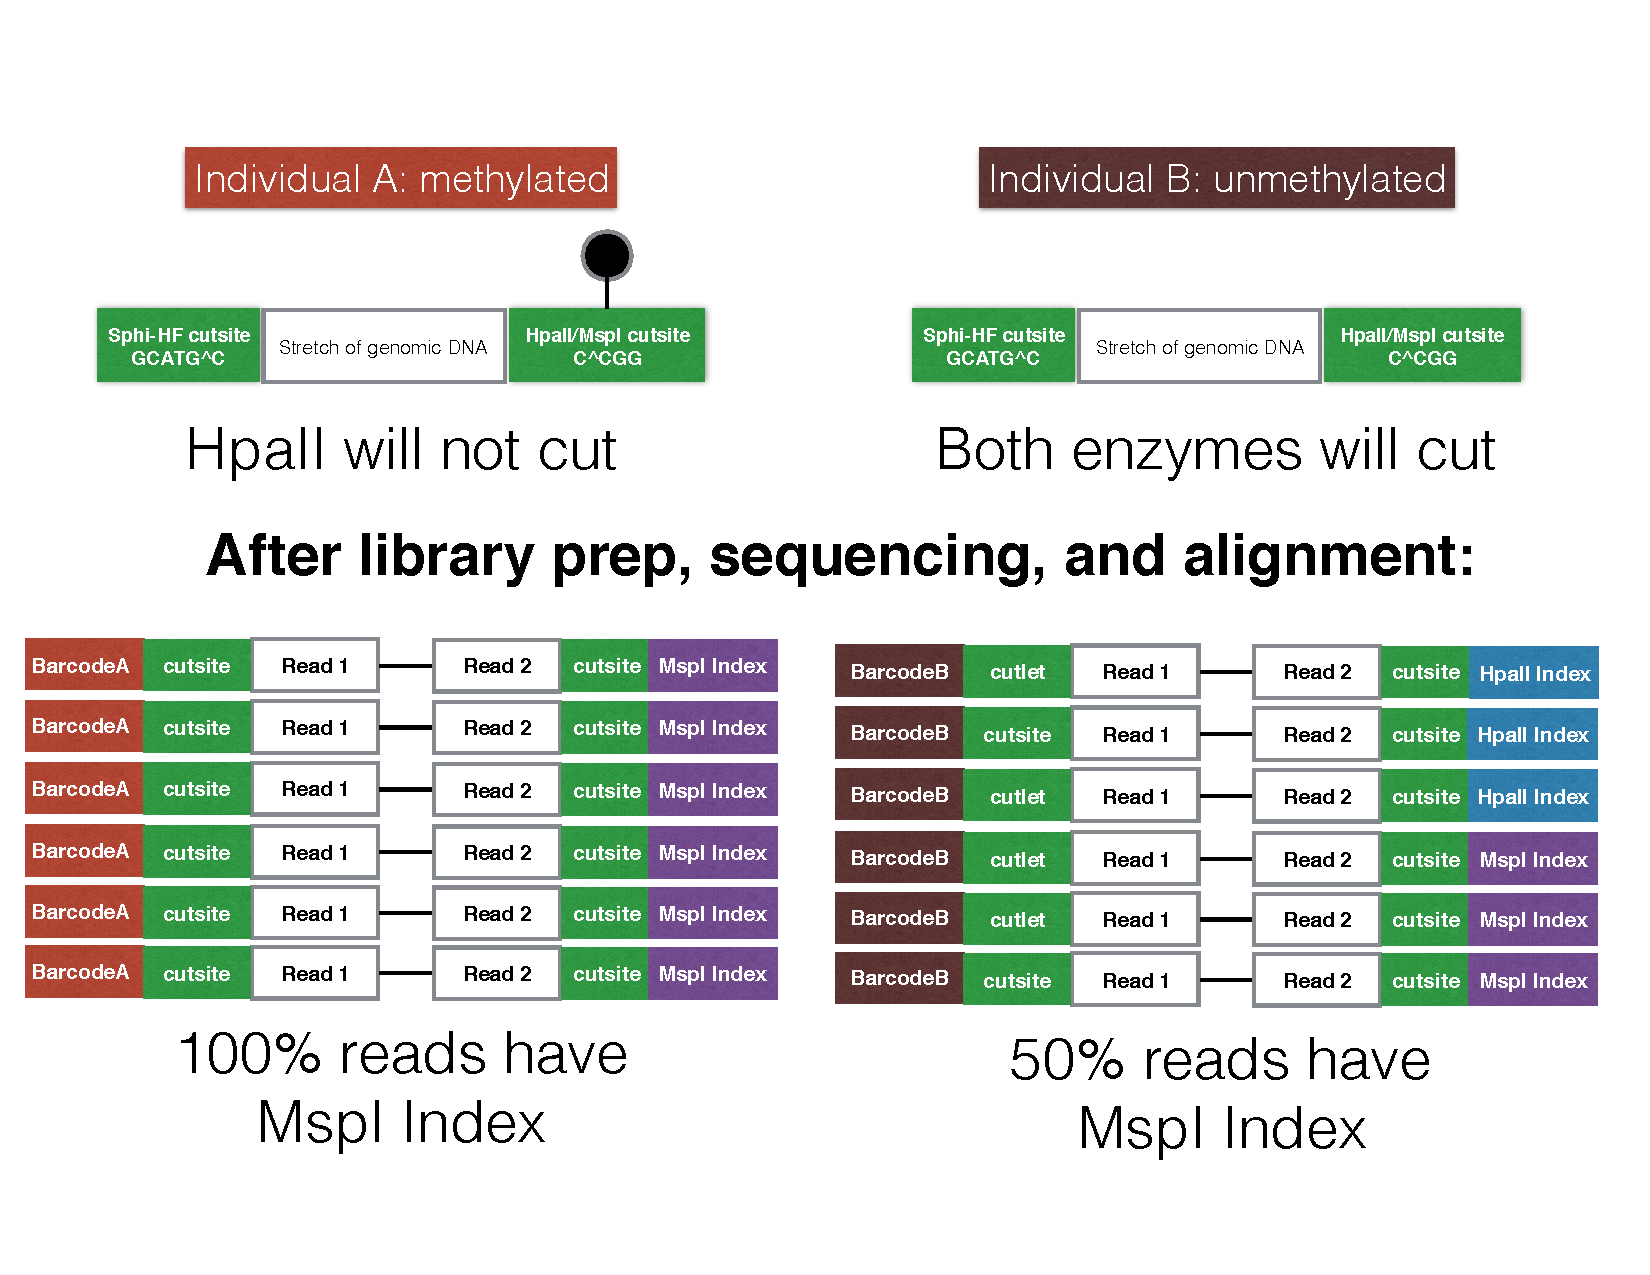
\includegraphics[width=5in]{./images/methylRAdd_bioinf.pdf}
			\caption{Overview of methylRAD bioinformatics}
		\end{figure}

	
	\clearpage
	\newpage

		\vspace{5mm}

	\subsection {Before you start: testing restriction enzymes with your DNA}
	\hl{TO DO}
	
	\subsection {Before you start: order oligos and anneal adapters}	
		We can order oligos through Eurofins Genomics through Fisher on Marketplace.  The PCR primers and oligos should be designed in a Word document according to the template outlined above.  The PCR primers should be universal.  You can modify the Rscript MakeddRADoligos\_SphI\_MspI.R for adapters for your specific restriction enzymes.  BE CAREFUL - ordering oligos is a large expense and it is easy to make mistakes.  I also suggest using CostAnalysis\_ddRAD.R to think about optimal cost-effective design for your study.  With very large sample sizes, it is worthwhile to invest in more barcodes.  
		
		When you receive them, you should resuspend the primers which is described in section \ref{Resuspend_Primer_Stocks}.  Then you organize the oligos in PCR strip-tubes or on a PCR plate so that it is easy to keep them in order.  The you should anneal the adapters together, which is described next and make aliquots, which is described in section \hl{ADD REF}.
		
		\subsection{Preparing working stocks of Oligos for ddRAD-seq (Annealing and Hybridization of Adapters) \label{oligo_ddRAD}}	
	
		\begin{adjustwidth}{0.25in}{0pt} Adapted from the Amplified restriction fragments for genomic enrichment protocol version 2.6 \end{adjustwidth}
			
		\noindent This protocol is meant to create working stocks of oligos to be used for ddRAD-seq. All of the adaptors and the primers have a barcode, so it is important to make sure that all of the adaptors and primers combinations have matching barcodes. 
	
			\noindent These adaptor sequences come in pairs and after annealing become one double-stranded adaptor. The barcodes are chosen from the Peterson protocol but may also be created using python scripts described in (Meyer \& Kircher, 2010). Further information on the python scripts can be found at 				(\url{<http://bioinf.eva.mpg.de/multiplex/>}). A second barcode will be attached on left side after PCR amplification (index). The second barcodes comes from the Peterson et al. 2012 flex adapters.

	\subsubsection{Peterson protocol}
	For the annealing buffer, might want to try NEBuffer 4 (B7004S).
	\begin{enumerate}
		\item To create Adapter P1 (P5 or "left"), combine each oligo 1.1 with its complementary oligo 1.2 in a 1:1 ratio in working strength annealing buffer (final buffer concentration 1x) for a total annealed adapter concentration of 40uM (for example, if purchased oligos are resuspended to an initial concentration of 100uM, use 40ul oligo 1.1, 40ul oligo 1.2, 10ul 10x annealing buffer and 10ul nuclease-free water). Do the same for oligos 2.1 and 2.2 to create the common adapter P2 (P7 or "right"). (100uM*40ul/(100uL final volume)=40uM)
		\item Combine in strip tubes or covered PCR plate:
			\begin{itemize}
				\item 40 uL P1.1 or P2.1 "top" Adapter (stock concentration 100 uM) 
				\item 40 uL P1.2 or P2.2 "Bottom" Adapter (stock concentration 100 uM) 
				\item 10 uL 10x Annealing Buffer or nuclease free water (buffer comes with T4 ligase from NEB)
				\item 10 uL H20
			\end{itemize}
		\item In a thermocyler, incubate at 97.5C for 2.5 minutes, and then cool at a rate of not greater than 3C per minute until the solution reaches a temperature of 21C. Hold at 4C.
		\item Setup of annealed primer stock in the freezer with each individual annealed adapter in a single tube setup in 96 well format. TREAT THESE LIKE GOLD- please take aliquots.
		
		\end{enumerate}
	\subsubsection{Schweyen protocol for P2/P7/"right" adapters with degenerate sequence}
		Hybridization of both strands was performed according to Peterson et al. (2012), with the exception of the temperature profile (97C for 5 min followed by a decrease in temperature of 2C per min in a 1.5-ml Eppendorf tube in a thermal block).
			
	\subsection {Before you start: choose barcodes and indexes}
	You should choose the barcodes and indexes you plan to use to tag and identify your individuals.  The "left" barcode is ligated on when the adapters are ligated; the "right" index is added in PCR.  Thus, ligation must be performed separately, but individuals with different "left" barcodes can be pooled together for size selection and PCR.   This can save \$ - another reason to think about your sampling design before starting.  
	
	For the indexes, llumina uses a green laser to sequence G/T and a red laser to sequence A/C. At each cycle at least one of two nucleotides for each color channel need to be read to ensure proper registration. It is important to maintain color balance for each base of the index read being sequenced, otherwise index read sequencing could fail due to registration failure. 
	
		\begin{figure}[h]
			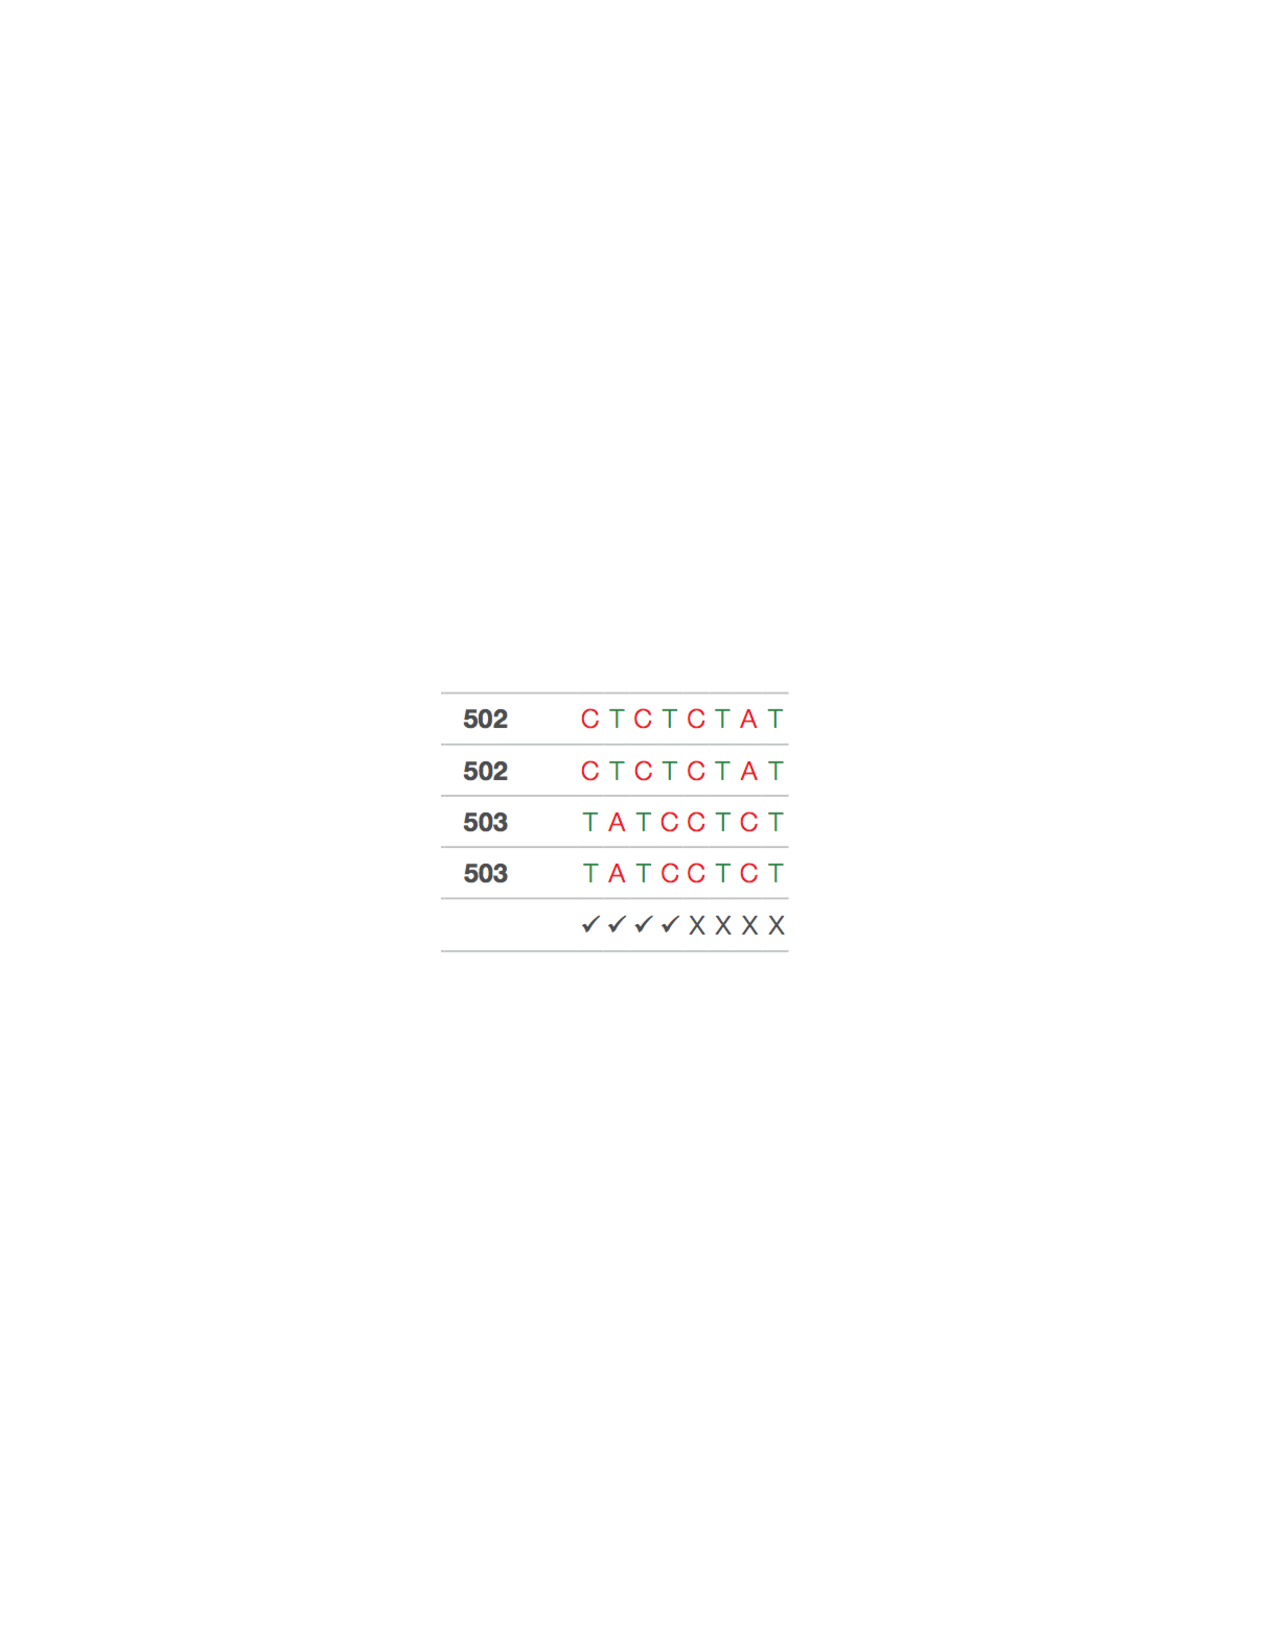
\includegraphics[width=3in]{./images/lowPlexityproblem.pdf}
			\caption{An overview of the low-plexity problem with Illumina}
		\end{figure}
    
    \begin{figure}[h]
			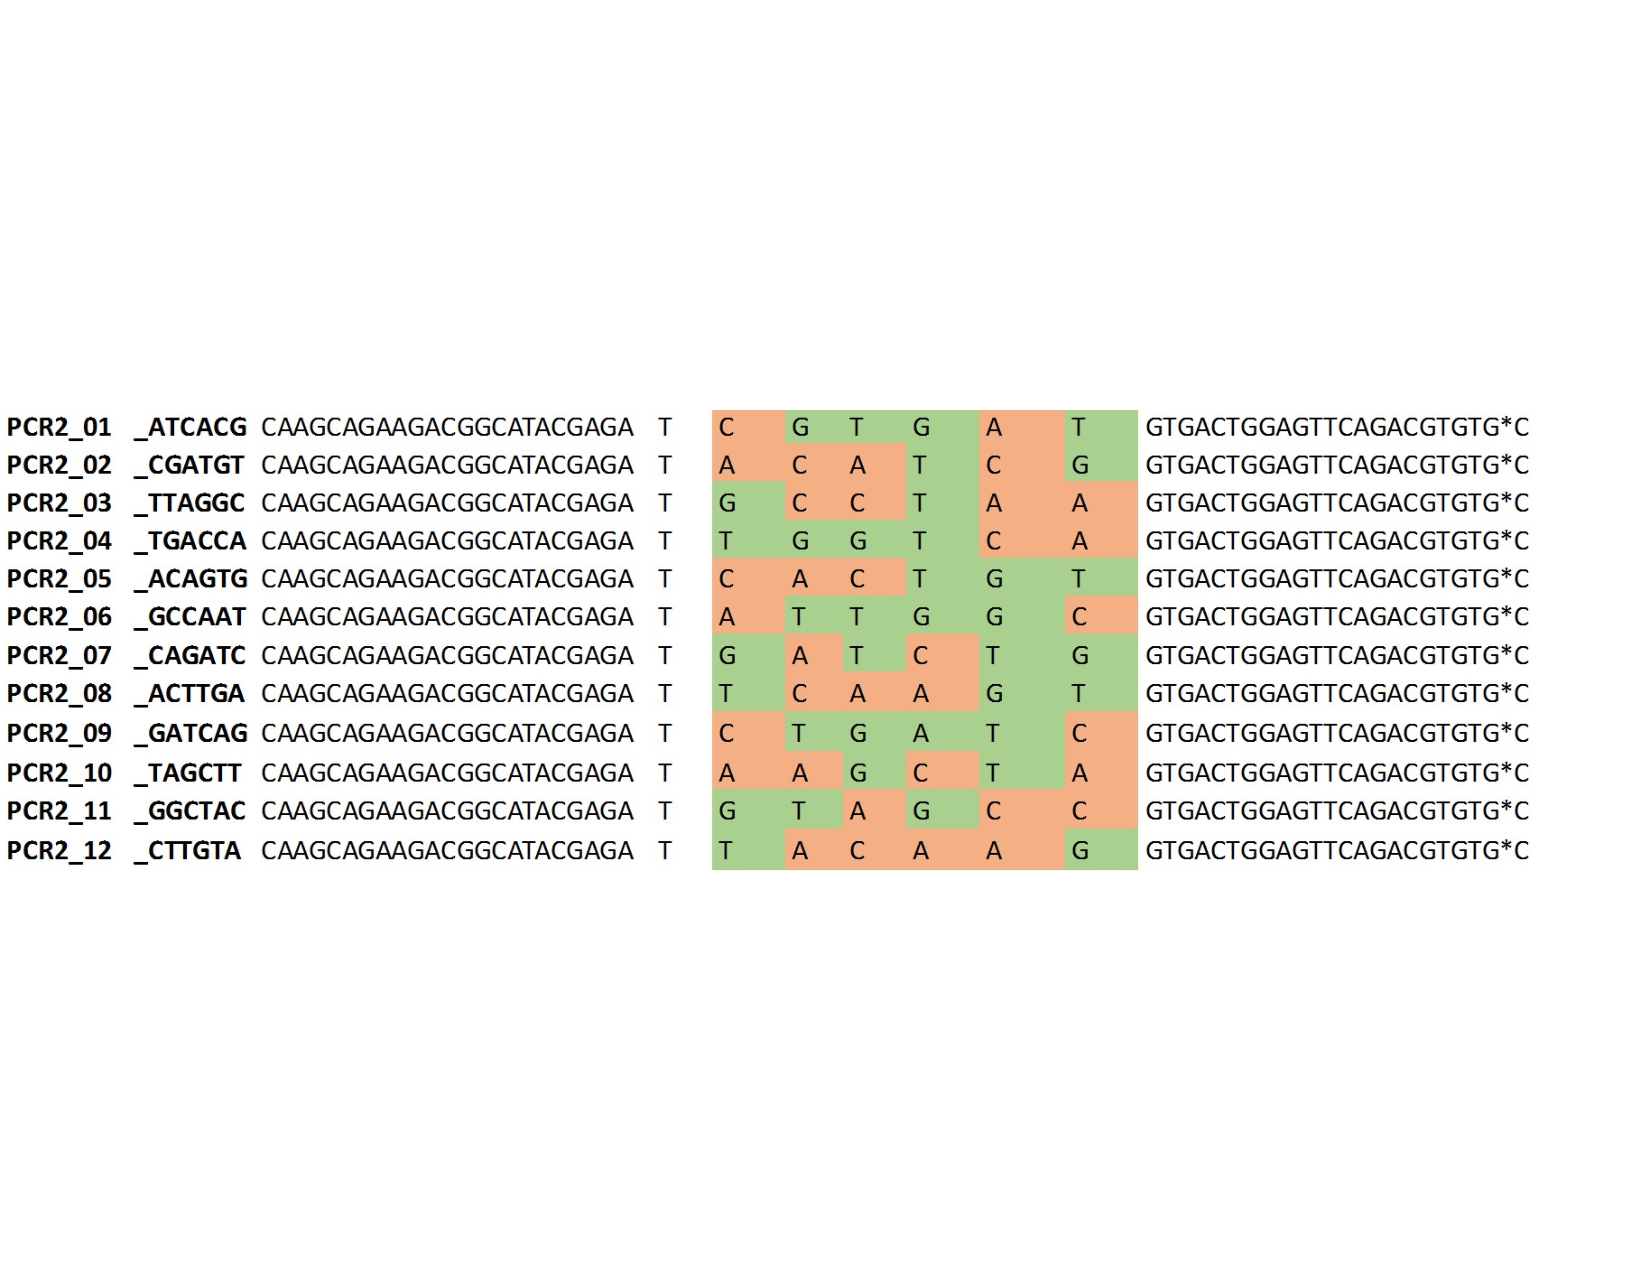
\includegraphics[width=3in]{./images/index_colorcode2.pdf}
			\caption{The Illumina indexes, by color code (Alan Downey-Wall).}
		\end{figure}
Illumina has a tool you can use to check your indexes. You can download the Experiment Manager from the Illumina website at http://www. illumina.com. Go to the Nextera DNA Library Preparation support page and click Downloads. A MyIllumina account is required. IEM will notify you if improper index combinations are used when creating a sample sheet for use with CASAVA, so it is highly recommended to create your sample sheet prior to performing library prep/ pooling. The IEM tool can be run on any Windows platform. Or, you can just do it by hand.
\clearpage

\subsubsection {Note on low plexity pooling}
For the SphI adapters and PCR2 indexes ordered on 201601, the following can be used for low plexity:
\begin{table}[]
\caption{Example of ddRAD LOW PLEXITY experimental barcoding setup}
\begin{center}
\begin{tabular}{c|c|c|c}
Individual & "left" barcode & "right" index MspI & "right" index HpaII  \\
I1 & SphI\_02 & PCR2\_09 & PCR2\_12 \\
I2 & SphI\_04 & PCR2\_09 & PCR2\_12 \\
I3 & SphI\_07 & PCR2\_09 & PCR2\_12 \\
\end{tabular}
\end{center}
\label{default}
\end{table}%
	
\subsubsection {Example of ddRAD experimental barcoding setup}
\begin{table}[]
\caption{Example of ddRAD experimental barcoding setup}
\begin{center}
\begin{tabular}{c|c|c|}
Individual & "left" barcode & "right" adapter \\
I1 & Sph01 & Index01 \\
I2 & Sph02 & Index01 \\
I3 & Sph03 & Index01 \\
I... & Sph... & Index01 \\
I16 & Sph16 & Index01 \\
I17 & Sph01 & Index02 \\
I18 & Sph02 & Index02 \\
I... & Sph... & Index02 \\
I32 & Sph16 & Index02 \\
I33 & Sph01 & Index03 \\
I34 & Sph02 & Index03 \\
I... & Sph... & Index03 \\
I48 & Sph16 & Index03 \\
\end{tabular}
\end{center}
\label{default}
\end{table}%

	\begin{table}[h]
					\caption[ddRAD example table]{Another example with 3 x 24 = 72 different barcode combinations (L is the left barcode and R is the right barcode)}
				\centering
				\begin{tabular}{ | c | c | c | c | c | c | c | c | c | }
				\hline
				\hl{L1 R1} & \hl{L9 R1} & \hl{L17 R1} & \hlc[green]{L1 R2} & \hlc[green]{L9 R2} & \hlc[green]{L17 R2} & \hlc[cyan]{L1 R3} & \hlc[cyan]{L9 				R3} & \hlc[cyan]{L17 R3} \\ \hline
				\hl{L2 R1} & \hl{L10 R1} & \hl{L18 R1} & \hlc[green]{L2 R2} & \hlc[green]{L10 R2} & \hlc[green]{L18 R2} & \hlc[cyan]{L2 R3} & \hlc[cyan]				{L10 R3} & \hlc[cyan]{L18 R3} \\ \hline
				\hl{L3 R1} & \hl{L11 R1} & \hl{L19 R1} & \hlc[green]{L3 R2} & \hlc[green]{L11 R2} & \hlc[green]{L19 R2} & \hlc[cyan]{L3 R3} & \hlc[cyan]				{L11 R3} & \hlc[cyan]{L19 R3} \\ \hline
				\hl{L4 R1} & \hl{L12 R1} & \hl{L20 R1} & \hlc[green]{L4 R2} & \hlc[green]{L12 R2} & \hlc[green]{L20 R2} & \hlc[cyan]{L4 R3} & \hlc[cyan]				{L12 R3} & \hlc[cyan]{L20 R3} \\ \hline
				\hl{L5 R1} & \hl{L13 R1} & \hl{L21 R1} & \hlc[green]{L5 R2} & \hlc[green]{L13 R2} & \hlc[green]{L21 R2} & \hlc[cyan]{L5 R3} & \hlc[cyan]				{L13 R3} & \hlc[cyan]{L21 R3} \\ \hline
				\hl{L6 R1} & \hl{L14 R1} & \hl{L22 R1} & \hlc[green]{L6 R2} & \hlc[green]{L14 R2} & \hlc[green]{L22 R2} & \hlc[cyan]{L6 R3} & \hlc[cyan]				{L14 R3} & \hlc[cyan]{L22 R3} \\ \hline
				\hl{L7 R1} & \hl{L15 R1} & \hl{L23 R1} & \hlc[green]{L7 R2} & \hlc[green]{L15 R2} & \hlc[green]{L23 R2} & \hlc[cyan]{L7 R3} & \hlc[cyan]				{L15 R3} & \hlc[cyan]{L23 R3} \\ \hline
				\hl{L8 R1} & \hl{L16 R1} & \hl{L24 R1} & \hlc[green]{L8 R2} & \hlc[green]{L16 R2} & \hlc[green]{L24 R2} & \hlc[cyan]{L8 R3} & \hlc[cyan]				{L16 R3} & \hlc[cyan]{L24 R3} \\ \hline
				\end{tabular}
	\end{table}

\subsubsection {Example of methylRAD experimental barcoding setup}
\begin{table}[]
\caption{Example of methylRAD experimental barcoding setup}
\begin{center}
\begin{tabular}{c|c|c||c|c|}
Individual & "left" barcode & "right" adapter MspI &  "left" barcode & "right" adapter HpaII\\
I1 & Sph01 & Index01 & Sph01 & Index02 \\
I2 & Sph02 & Index01 & Sph02 & Index02 \\
I3 & Sph03 & Index01 & Sph03 & Index02 \\
I... & Sph... & Index01 & Sph... & Index02 \\
I16 & Sph16 & Index01 & Sph16 & Index02 \\
I17 & Sph01 & Index03  & Sph01 & Index04\\
I18 & Sph02 & Index03 & Sph02 & Index04\\
I... & Sph... & Index03 & Sph... & Index04\\
I32 & Sph16 & Index03 & Sph16 & Index04\\
\end{tabular}
\end{center}
\label{default}
\end{table}%

\clearpage
\newpage

	\subsection {Reagents and Equipment}

		\begin{itemize}[leftmargin=0.5in]
			\item[--] Note that we chose these enzymes because they were not sensitive to methylation.
			\item[--] Restriction Enzyme 1: (depends) SphI-HF (NEB, 20,000 units/ml) R3182S 
			\item[--] Restriction Enyzme 2: (depends) MspI (R0106S), HpaII (R0171S) or (MluCI NEB, 10,000 units/mL R0538S)
			\item[--] 10x Concentrate Enzyme Buffer (part of the enzyme package)
			\item[--] T4 DNA Ligase (NEB, 400,000 units/mL) M0202L 
			\item[--] 10x T4 buffer (part of the Ligase package)
			\item[--] BioRad Iproof High Fidelity DNA polymerase Cat \# 172-5301 (424 for 250 uL [500 units])
			\item[--] DMSO (part of the package of the Iproof polymerase)
			\item[--] MgCl2 (part of the package of the Iproof polymerase)
			\item[--] 1 mg/mL BSA (BSA may not be needed, it is now incorporated in the enzyme buffer, but we keep it in anyway) Cat \# BP675-1 				Fisher  
			\item[--] 1 M NaCl (follow reagent recipe)
			\item[--] dNTP Cat \# R0181 Thermo Scientific
			\item[--] SphI-HF adaptors (add page number for ordering adaptors) 
			\item[--] MluCI adaptors (add page number for ordering adaptors)
			\item[--] Milli-Q Water
			\item[--] Thermal Cyclers 
			\item[--] 96 well plates and strip caps or PCR strip tubes Cat \# AB-0600 Thermo Scientific
			\item[--] 1.5 microcentrifuge tubes for PCR mixes (any 1.5 microcentrifuge would work)
			\item[--] Full plate centrifuge (if using a full plate)
			\item[--] Qubit (we used the Qubit 3.0 Cat \#Q33216) and special tubes Qubit Cat \# Q32856 or VWR Cat \# PCR-05-C
			\item[--] Note that the concentrations used in our protocol are from a Qubit, which is more accurate than a Nanodrop (the Nanodrop estimates concentrations 2-10x higher than the Qubit).
			Agarose and gel electrophoresis materials (see Section Quality assessment of DNA and RNA with gel electrophoresis)
			\item[--] 0.1X TE
			\item[--] Homemade DNA beads (please see the Home made bead protocol if you need to make them) or 
			\item[--] EtOH molecular grade
			\item[--] QIAquick Gel Extraction Kit (\#28704)
		\end{itemize}

		\vspace{5mm}

	\subsection {Things to do before starting}

		\begin{itemize}[leftmargin=.5in]
			\item Make sure the adaptors are annealed, and also make sure the adaptors and the primer mix are easily accessible in plate format. Please see the section above.	
			\item Be familiar with the Pippin Prep and how to use it.
			\item Know what size range you want to select - see details in size selection section.	 To do this, you should have a plan for sequencing.		
			\item Make sure all of the supplies needed for the protocol are present and are sufficient for the number of samples that you will be processing. This protocol is long and it has few stopping steps. 
			\item Make sure the enzyme combination is the best for your organisms. The types of enzymes and the digestion length should be checked at least one time prior this protocol. 
		\end{itemize}

	
	\subsection {Protocol}

		\vspace{5mm}

\subsubsection {1. Restriction Double Digest ($\sim$ overnight)}

From NEB website: There are several key factors to consider when setting up a restriction endonuclease digestion. Using the proper amounts of DNA, enzyme and buffer components in the correct reaction volume will allow you to achieve optimal digestion. By definition, 1 unit of restriction enzyme will completely digest 1 $\mu$g of substrate DNA in a 50 $\mu$l reaction in 60 minutes. This enzyme : DNA : reaction volume ratio can be used as a guide when designing reactions. However, most researchers follow the "typical" reaction conditions listed, where a 5--10 fold overdigestion is recommended to overcome variability in DNA source, quantity and purity. NEB offers the following tips to help you to achieve maximal success in your restriction endonuclease reactions. NEB recommends 10 units restriction enzyme, 1$\mu$g DNA, 1X NEB Buffer (5$\mu$L), and 1 hour incubation time.

DNA (measured with the Qubit) should ideally be at a minimum total amoung of 1.5 $\mu$g and no more than 2.5 $\mu$g. For example, you could use 10$\mu$L of 150-250 ng/$\mu$L of DNA.  Keep on ice.  Note that your DNA needs to be concentrated at least 125 ng/$\mu$L for this protocol (2,500 ng desired/125ng/$\mu$L = 20$\mu$L + may need 5-7uL master mix depending on enzymes).

For each sample prepare a master mix I (Table 1), mix by vortexing and then centrifuge. For these and all other reactions make sure to prepare an excess of mix to accommodate multiple rounds of pipetting, particularly if you are working with whole plates. Because the enzymes are stored in glycerol and other viscous solutions, a substantial volume is lost through adhesion to the outside of pipette tips. We suggest making more than what you think you will need (this may be overkill, if you have fewer columns than just do one extra per column).


			\begin{table}[h]
				\centering
				\begin{tabular}{ | c | >{\centering\arraybackslash} m{10em} |}
					\hline
					\cellcolor{gray}{\bf Reagent} & \cellcolor{gray}{\bf Number of samples 1X (uL)}  \\
					\hline
					20 units of Enzyme 1 & (Calc) \\
					20 units of Enzyme 2 & (Calc) \\
					(10x Concentrate Enzyme Buffer) & 3 ul\\
					Genomic DNA (1.5-2.5 ug) & (Calc) \\
					Molecular grade H20 to make a final volume of 30 uL & (Calc) \\
					\hline
		
				\end{tabular}
			\end{table}

			\noindent {\bf Table 1:} Reagents and volumes for Restriction Digest master mix I (30 uL prepared per sample). Note: The original protocol listed 10xT4 Buffer instead of the 10X Concentrate Enzyme Buffer. We think this may have been a typo. 10xT4 Buffer is designed to work with the Ligase (we use Ligase in the following section) and the 10x Concentrate Enzyme Buffer is designed to optimize the enzyme.  See NEB website.

			\begin{enumerate}
			\item Incubate samples at 37C overnight. NOTE THAT MspI CANNOT BE KILLED BY HEAT.  SUGGEST PROCEEDING IMMEDIATELY TO BEAD WASH.
			\item After incubation, let reaction cool to room temperature during this time also remove the AMPURE XP beads from the fridge and let them warm to room temperature
			\item Add 45 uL of AMPURE XP to each reaction, mix with pipetting 10 times, and then let incubate for 5 mins on the bench
			\item Place plate onto the magnet plate and let the beads separate for 5 mins
			\item Carefully remove the supernatant from each well and discard
			\item Note that you will not be able to remove all of the supernatant without disturbing the beads. It's best to leave about 5 uL remaining in each well
			\item Leaving the plate in the magnet, wash the reaction by adding 200 uL of FRESH 70\% ethanol { \bf 70\% ethanol should be mixed that day!}
			\item Remove and discard ethanol and repeat with a second ethanol wash. (From Gold Lab Protocol: Puritz prefers to use only 150 uL of ethanol for second wash. Hollenbeck prefers to use only 1 wash step)
			\item After final wash, let plates air dry for 5-10 mins. All ethanol needs to be evaporated, but beads should not be overdried.
			\item Remove plate from magnet and add 30 uL of molecular grade H2O to each well and incubate for 5 mins. Make sure that water comes into contact with beads by mixing well with pipet
			\item Place plate back on magnet and let it separate for 2 minutes, then remove supernatant and transfer to clean plate
			\item If doing a second set of digestion, repeat steps 4-11.

			\end{enumerate}
			
		
\subsubsection {Digest Quantification}
		Check quantification of DNA on Qubit. For extra accuracy, reread standards every 48 samples. These numbers will be used in next step.
		
		Typically get between 10ng/uL and 100ng/uL.
		
		Optional sanity check: Run your restriction digest product on a gel and compare to genomic DNA.

\subsubsection {Adaptor Ligation ($\sim$2-3 hours) - proceed directly to pooling after}

		\begin{enumerate}
			\item Thaw adaptors (or the L and R adaptors). Have these adaptors annealed and easily accessible in plate format.
			\item For each sample, calculate the amount of template needed for 100 ng of DNA and calculate the amount of H20 to add to this amount by using the formula 22.2-(ul of Template)= uL of $H_20$ (total final volume should be 22.2 uL). If samples are of low DNA concentration, this can be adjusted to 31.2-(ul of Template)= uL of $H_20$ for all samples.
			\item Place the correct amount of $H_20$ and then DNA into ligation plate A. This will take some time. Take out T4 ligase buffer to thaw during this time.
			\item Transfer 2 uL of ``left" adapter to each reaction.  PAY ATTENTION TO YOUR DESIGN.
			\item Transfer 2 uL of ``right" adapter to each reaction.  PAY ATTENTION TO YOUR DESIGN.  If the right adapter is universal, it can be incorporated into master mix.
			
			\item Total ligation mix as follows:
			\begin{table}[h]
				\centering
				\begin{tabular}{| c | >{\centering\arraybackslash}m{10em} |}
				\hline
				\cellcolor{gray}{\bf Reagent} & \cellcolor{gray}{\bf Number of samples 1X (uL)}  \\
				\hline
				UNIQUE DNA template & 22.2 \\
				UNIQUE ``left" universal adapter & 2 uL \\
				UNIQUE ``right" universal adapter & 2 uL \\
				MASTER (NEB Buffer \#4 10X) ligation buffer & 3 uL \\
				MASTER T4 ligase (Add this last) & 0.8 uL \\
				\hline
				\end{tabular}
			\end{table}
			
			\item Add 3.8 uL of master mix to each reaction, as quickly as possible
			\item Incubate on bench top for one hour, then place in thermocycler and heat-kill at 65C for 10 min. After the heat-kill, cool the solution at 2C per 90 seconds until it reaches room temperature. Hold at 4C or place in fridge.  
			
			\item Optional sanity check: you should have 100ng/30ul=3.33 ng/uL of DNA.  Use Qubit HS dsDNA kit to double check.
			
		\end{enumerate}

			\newpage
			
\subsection{Pooling and Beadwash}
	Set up your pools for size selection on the Pippin Prep.  You should have experience using the Pippin before you perform this step.
	\begin{enumerate}
		\item After ligation, it is safe to pool samples within one index. Collect all 30 uL from each well and place it into a single 1.5 mL tube (Use a 2.0 mL tube if using 40 uL ligations).  If you are using 16 barcodes within an index, this is 16*30 = 480 uL.  
		\item Mix each pool with pipetting or gentle vortexing.  If it is a large volume split each into equal aliquots according to the number of replicate size selections.  (These replicates will be combined in last step.  It doesn't affect the total amount of beads used, and you can choose to do fewer if you don't have a lot of product).
		\item Add 1.5X uL of AMPURE XP to each aliquot, mix with pipetting 10 times, and then let incubate for 5 mins on the bench.  For instance, if you did two replicate size selections of a pool with 16 barcodes, each one would be 480ul/4 = 120 uL of template and 180 uL of beads.
		\item Place tube onto the magnet bar and let the beads separate for 5 mins
		\item Carefully remove the supernatant from each tube and discard
		\item Sometimes pulling tube upwards and tilting bottom towards the magnet allows for complete supernatant removal. If not, leave a few uL.
		\item Leaving the tubes in the magnet, wash the reaction by adding 500 uL of FRESH 70\% ethanol {\bf 70\% ethanol should be mixed that day!}. Volume is approximate but should cover all beads
		\item Remove ethanol, let tubes air dry for 2 mins. All excess ethanol needs to be evaporated, but shiny beads are OK and beads should not be overdried. Pippin is sensitive to EtOH so err on side of more dry.

		\item Remove tubes from magnet and add 30 uL of TE buffer to each tube and incubate for 5 mins. Make sure that water comes into contact with beads by mixing well with pipet or gentle vortexing
		\item IF DOING REPLICATES: Remove tubes from magnet and add 30 uL of molecular grade H2O to each tube and incubate for 5 mins. Make sure that water comes into contact with beads by mixing well with pipet or gentle vortexing
    \item IF NOT DOING REPLICATES: Remove tubes from magnet and add 30 uL of TE to each tube and incubate for 5 mins. Make sure that water comes into contact with beads by mixing well with pipet or gentle vortexing. (We use TE here because it helps the DNA stay in the well of the Pippin Prep).
		\item Place tubes back on magnet and let beads separate for 2 minutes, then remove supernatant and transfer to a clean 1.5 mL tube.  If you used replicates, pool within each index. This means going from multiple aliquots to one tube for each index.
		\item IF YOU USED REPLICATES, DO THE FOLLOWING STEPS TO POOL.  IF NOT, YOU ARE DONE. If you used replicates, add 1.5X uL of AMPURE XP to each tube, mix with pipetting 10 times, and then let incubate for 5 mins on the bench.  
		\item Place tubes onto the magnet bar and let the beads separate for 5 mins
		\item Carefully remove the supernatant from each tube and discard.  Sometimes pulling tube upwards and tilting bottom towards the magnet allows for complete supernatant removal. If not, leave a few uL.
		\item Leaving the tubes in the magnet, wash the reaction by adding ~500 uL of FRESH 70\% ethanol. Volume is approximate but should cover all beads
		\item Remove and discard ethanol, and let plates air dry for 2 mins
		\item All ethanol needs to be evaporated, but beads should not be overdried. Pippin is sensitive to EtOH so err on side of more dry.
		\item Remove tubes from magnet and add 20 uL of TE buffer to each tube and incubate for 5 mins A. Make sure that water comes into contact with beads by mixing well with pipet or gentle vortexing
		\item Remove tubes from magnet and add 20 uL of TE to each tube and incubate for 5 mins A. Make sure that water comes into contact with beads by mixing well with pipet or gentle vortexing.  We use TE here because it helps the DNA stay in the well for the pippin.
		\item Place tubes back on magnet and let beads separate for 2 minutes, then remove supernatant and transfer to a clean 1.5 mL tube
		\end{enumerate}

	\begin{figure}[h]
			
\includegraphics[width=0.5in]{./images/Safe_Stop.pdf}
			\caption[ddRAD Safe Stop after pooling]{SAFE STOP POINT.  Store at 4C for a month, or -20C for longer.  It is important to save this, as all of this product is not used for the PCR, and if the results of the PCR do not look good, you can start again from this step.}
		\end{figure}

\clearpage

\subsection{ Size selection ($\sim$ 2 hours)}
 We use a Pippin Prep to do size selection. Pippin works in a similar way to typical gel electrophoresis, but uses standardized gel cassettes and automated size selection, rather than a hand-poured gel and manual excision of fragments from a gel. It is necessary to specify a size range of fragments that you would like represented in the final genomic library for sequencing. The target size range can be adjusted to modify the number of fragments expected for sequencing. Because techniques such as this typically result in a negative relationship between fragment size and number, selecting larger fragments should decrease the final number of fragments in the template and increase the coverage depth of these regions after sequencing. Similarly, decreasing the size interval selected will also reduce the number of fragments and increase coverage. The number of fragments produced is also in part a function of genome size, so awareness of your organism`s genome size is helpful in making an appropriate choice for size selection (see Fig. 3 of Alex`s protocol, and Figure 1 in SCHWEYEN 2014).  Most people use a 100-150 bp range somewhere between 250 and 500 bp in total fragment length (meaning that we might select, as an example, fragments that are 300 - 400 bp in length).  With 8 samples per index, we found a 200 bp range gave better results because more DNA was left after size selection (300-500 bp).  With more samples per index, a 150 bp range would probably be OK.

Dr Lotterhos has an R script that can be used to do an in silico digest of a genome.  It is called ddRADoysterdigestion.R (for C. gigas oyster) but can be applied to any genome.  The basic code is in a post on her blog.  You should calculate your size range based on the the number of fragments in your selected size range, and your plan for sequencing (the number of paired-end reads and their read length and the total number of bases captured).


			\begin{figure}[h]
				\begin{center}
					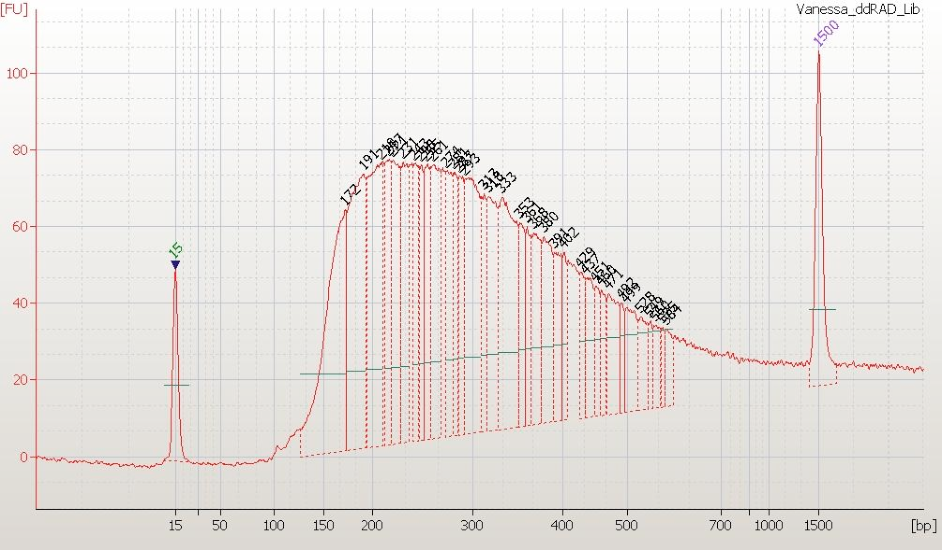
\includegraphics[height=2.5in]{./images/afterPCR_Bioanalyzer.pdf}
					\caption{Bioanalyzer results from a library prior to size selection but after PCR amplification.}
				\end{center}
			\end{figure}

			\begin{figure}[h]
				\begin{center}
					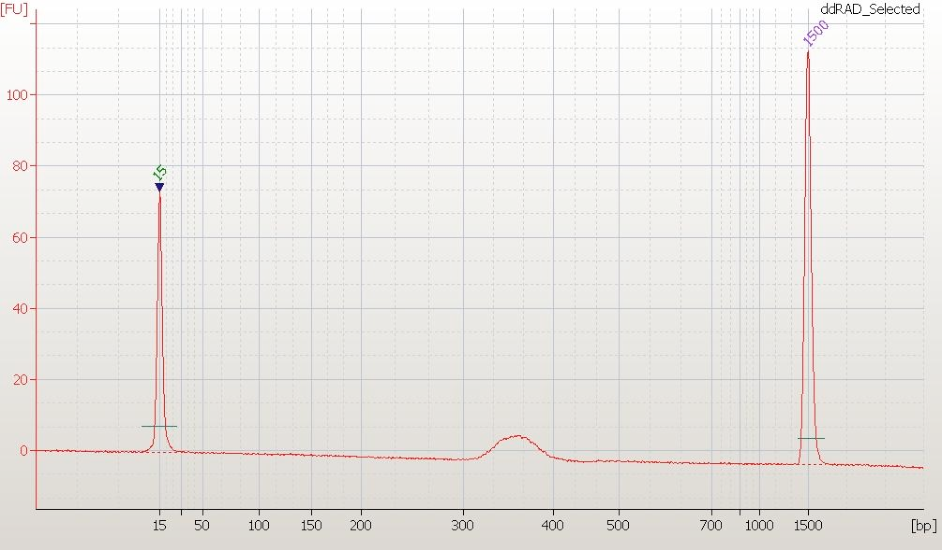
\includegraphics[height=2.5in]{./images/afterPippin_Bioanalyzer.pdf}
					\caption{Bioanalyzer results from a library after amplification and size selection with Pippin Prep.}
				\end{center}
			\end{figure}
\clearpage
\newpage

\noindent {\bf NOTE: } We tried and tested gel size selection and decided that this approach should be only used if Pippin is not a possibility.  After cutting fragments from the gel, purifying them, and re-running them on another gel, we found that the gel had a tails outside the targeted fragments size \hl{(Figure \#)}.  Nothing we tried could get rid of these artifacts. We tried to add a denaturing step and a bead wash to remove artifacts or contaminants \hl{(Figure \# and \#)}, but we continued to have tails outside the desire fragment 				range. This may be due to differences on the movement of fragments. 

				\begin{figure}[h]
					\begin{center}
						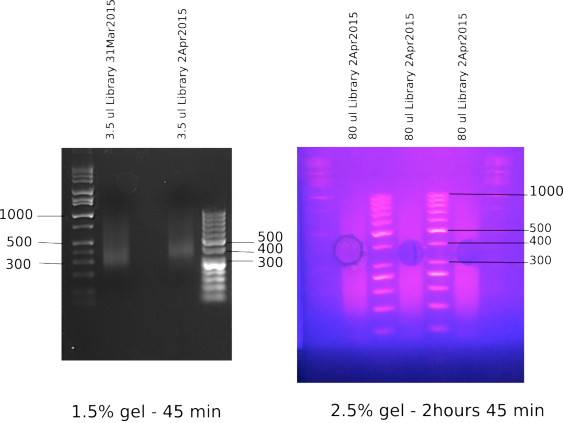
\includegraphics[height=2.5in]{./images/gel_sizeselection.pdf}
						\caption[Gel size selection] { Gel size selection (right) 2.5\% gel ran for 2 hours and 45 minutes. The fragments in the range of 300-400bp were removed using a pipette tip. (left) Gel picture of the PCR products after the gel size selection.}
					\end{center}
				\end{figure}


				\begin{figure}[H]
					\begin{center}
						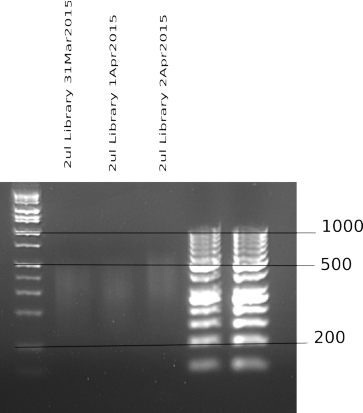
\includegraphics[height=2.5in]{./images/gel_sizeselection_denaturelast.pdf}
						\caption[Denaturing before size selection] {Gel picture of the libraries after amplification (PCR), gel size selection and a 							denaturing step.}
					\end{center}
				\end{figure}
		
				\begin{figure}[H]
					\begin{center}
						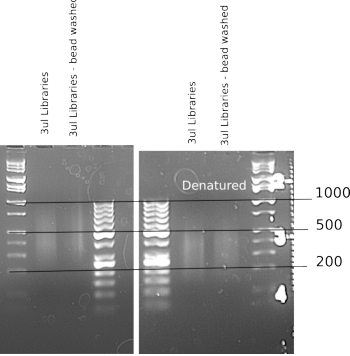
\includegraphics[height=2.5in]{./images/gel_sizeselection_denaturefirst.pdf}
						\caption[Denaturing after size selection] {Gel picture of libraries that were denatured before size selection and ran in a final gel 						(left). An additional denaturing step prior to the final gel picture was done for comparison (right). }
					\end{center}
				\end{figure}

\clearpage

				\newpage

\subsubsection{ Targeted Index PCR Amplification ($\sim$8 hours including checking on gel and final beadwash)}
Following Ligation, pooled groups of samples with individual left adapters are amplified with a unique right adapter. The right adapter would add a unique barcode to the right side that would allow all of the pools to be pooled in one lane for sequencing. To ameliorate stochastic differences in PCR production of fragments in reactions, we run 3-8 replicate reactions per right barcode group, and later combine them.  NOTE THAT WE USE IPROOF HF-TAQ, which is cheaper than the Phusion Taq that most people are using. There are alternative polymerases for ddRAD-seq libraries that may be equally or more effective than Iproof Taq. NEB has good alternatives. 

	\begin{enumerate}
		\item For 8 individuals per index after Pippin, we've measured 1000-2000 ng/mL (1-2 ng/uL) and this works well with Vanessa's protocol.
		
		\item Prepare the following Master Mix. Prepare an individual master mix for each individual right adapter according to the number of replicate PCRs that you want to run. WE SUGGEST 6 REPLICATES. You will notice two protocols: Vanessa protocol and Peterson protocol.  Vanessa protocol works better with 4-8ng of DNA total, we haven't yet tested larger amounts of DNA. The Peterson protocol is included as a reference.
		
				\vspace{2mm}
				
				\begin{table}[h]
					\centering
					\begin{tabular}{ | c | >{\centering\arraybackslash} m{10em} |}
						\hline
						\cellcolor{gray}{\bf VANESSA PROTOCOL} & \cellcolor{gray}{\bf Number of samples 1X (uL)}  \\
						\hline
						ddH2O & 10.4 (or calc) \\
						5x Iproof buffer & 4 \\
						dNTP (10 mM) & 0.4 \\
						MgCl2 (50 mM) & 0.4 \\
						PCR Primer 1 (10 uM) universal & 0.35 \\
						PCR Primer 2 (10 uM) index specific & 0.35 \\
						Iproof Taq & 0.2 \\
						DMSO & 0.15 \\
						DNA pooled template (after size selection) & 4 (or calc) \\

						\hline	
					\end{tabular}
				\end{table}
				

				\begin{table}[h]
					\centering
					\begin{tabular}{ | c | >{\centering\arraybackslash} m{10em} |}
						\hline
						\cellcolor{gray}{\bf PETERSON PROTOCOL} & \cellcolor{gray}{\bf Number of samples 1X (uL)}  \\
						\hline
						ddH2O & 1.75 (or calc) \\
						5x Iproof buffer & 4 \\
						dNTP (10 mM) & 0.4 \\
						MgCl2 (50 mM) & 0.5 \\
						PCR Primer 1 (10 uM) universal & 2 \\
						PCR Primer 2 (10 uM) index specific & 2 \\
						Iproof Taq & 0.2 \\
						DMSO & 0.15 \\
						DNA pooled template (after size selection) & 5 (or calc) \\

						\hline	
					\end{tabular}
				\end{table}

				\vspace{3mm}

	\item Thermocycler profile for this PCR: 98C for 1min; 12 cycles of: 98C for 10s, 62C for 30s,
				72C for 30s; final extension at 72C for 10 min. Hold at 4C.
				
	\item Check if the amplification of the PCR product has gone well by running 2ul of the PCR product in a 2\% agarose gel (you can use the same gel to run the final pooled PCR product cleaned made in the following step).  We have found that if there is a lot of primer-dimer, you can get a higher qubit reading, even though the PCR worked poorly.
	\end{enumerate}
	
\subsubsection{Final beadwash and pooling of PCR products}	
	\begin{enumerate}
	\item Combine the replicate PCR reactions into a single 1.5 mL tube (6 * 16ul = 96 uL)
	\item Add 144 uL (96*1.5 uL) of AMPURE XP to each aliquot, mix with pipetting 10 times, and then let incubate for 5 mins on the bench.
	\item Place tube onto the magnet bar and let the beads separate for 5 mins
	\item Carefully remove the supernatant from each tube and discard.  Sometimes pulling tube upwards and tilting bottom towards the magnet allows for complete supernatant removal. If not, leave a few uL.
	\item Leaving the tubes in the magnet, wash the reaction by adding ~500 uL of FRESH 70\% ethanol A. 70\% ethanol should be mixed that day! Volume is approximate but should cover all beads
	\item Remove ethanol and repeat wash
	\item Remove ethanol, let tubes air dry for 5-10 mins. All ethanol needs to be evaporated, but beads should not be overdried
	\item Remove tubes from magnet and add 30 uL of molecular grade H2O to each tube and incubate for 5 mins
	\item Make sure that water comes into contact with beads by mixing well with pipet or gentle vortexing
	\item Place tubes back on magnet and let beads separate for 2 minutes, then remove supernatant and transfer each index to a clean 1.5 mL tube.
	\item These four tubes are your final library
	\item Prepare working solution for the Qubit by combining 199 uL of stock solution with 1 uL of dye for every reaction.
	\item Collect 0.5 ml sample tubes, one for every reaction and two for standards
	\item Prepare standards by combing 190 uL of working stock with 10 uL of standard (stored in refrigerator)
	\item Turn on Qubit by touching screen and press button to read new standards. Follow prompts on screen.
	\item Prepare 6 samples for quantification by putting 199 uL of working stock with 1 uL of sample in a 0.5ml tube
	\item Use Qubit to measure DNA content, remembering to press button to calculate stock concentration and to press button to save data before switching tube and pressing ``read new sample"
	\item If each index is between 5-100 ng/uL, celebrate. You are finished.
	\end{enumerate}
				
\subsubsection{Check libraries on Bioanalyzer}
	\begin{itemize}
		\item Bioanalyzer is in Vollmer Lab.  When we get a key, we will keep in in the drawer with the pens.
		\item The password for the computer is under the keyboard.
		\item Have ready 350 uL RNAase free water, and pipettes and tips.  Plan time to let reagents get to room temperature.
		\item Clean the electrodes: (1) Fill one well of the electrode with 350 uL RNAase-free water. (2) Place the electrode cleaner in the bioanalyzer. (3) Close the lid and let sit for 5 mins. (4) Afterwards, leave the lid open for at least 30 sec to allow for evaporation.
		\item There are DNA chips and RNA chips. They are actually the same thing, but there are some differences in the calculations done on the machine.  The RNA chips are slightly cheaper.  You can only use 12 wells on a chip at a time, for example if you only use 3 wells then that chip is done.
		\item Follow instructions that come with the chip.
		\item	The gel-dye mix is only good for 4 weeks, so don't make too much at a time.
		\item When you close the chip priming station, MAKE SURE IT CLICKS.
		\item The chip vortexer is kind of freaky.  The chip will squish into it. Make sure to test it with the electrode cleaner first so you can see how it works.
	\end{itemize}

\subsubsection{Quantify adapters with Kapa Kit}
	\hl{TO DO}					

\clearpage
\newpage
\section{RNA Library Prep}

	\noindent (Adapted from the NEBNext rRNA Depletion Kit manual, NEBNext Ultra RNA Library Prep Kit for Illumina manual, and the NEBNext Multiplex Oligos for Illumina manual)
	
	\vspace{3mm}
	
	\subsection{Introduction}
	
	\vspace{2mm}
	
	\noindent This protocol is designed to build barcoded cDNA libraries from DNA-free RNA. The protocol uses three kits: NEBNext rRNA Depletion Kit, 	NEBNext Ultra RNA Library Prep Kit for Illumina, and the NEBNext Multiplex Oligos for Illumina kit. Extracting total RNA results in a product made up of 	a high proportion of ribosomal RNA (rRNA). When building a cDNA library, we are interested in the mRNA and non-coding intronic and intergenic RNA 	that make up only a small proportion of our total RNA extraction. Therefore, to begin making a cDNA library, we first need to remove as much of the 		rRNA as we can. This is done in the first section of the protocol with the NEBNext rRNA Depletion Kit. This kit reduces the amount of rRNA that is found 	in the sample. NOTE: your initial concentration of RNA should be between 100 ng - 1 ug in 12 uL. We recommend the higher side .75 - 1 ug due to how 	much will be depleted in this step of the protocol ($\sim$10\% of starting product will be left i.e. start with 750 ng after depletion you should have 75 ng). 
	
	\vspace{2mm}
	
	\noindent Once the rRNA has been depleted, we can move on to the building of our cDNA libraries, which is done using the NEBNext Ultra RNA Library 	Prep Kit (if interested in having strand specific information this kit would be substituted with the NEBNext Ultra Directional RNA Library Prep Kit 		\#E7420S). This kit creates cDNA libraries that will be ready for next-generation sequencing. 
	
	\vspace{2mm}
	
	\noindent Finally, the NEBNext Multiplex Oligos for Illumina provide Index primers 1-12 that will be used to provide unique identifiers for samples being 	sequenced in the same lane on the sequencer. By doing this, you can sequence many samples within a single lane, which reduces sequencing costs. 	However, you do not want to have too many samples in a single lane because this can reduce the overall sequencing coverage of each sample i.e. 		Illumina HiSeq 	2000 produces 100 - 200 million reads per lane and Illumina HiSeq 2500 produces 100-150 million reads per lane. Based on how many 	reads you want per sample, you can use this information to determine how many samples to put into each lane. 
	
	\vspace{2mm}
	
	\noindent If this is your first time building a cDNA library or using this protocol in particular, it is important to go through the protocol with just one sample 	to ensure you know the steps well. Each step is temperature sensitive and needs to be carried out quickly. Therefore, walking through the protocol once 	will allow you to learn the steps before using too many samples. 
	
	\vspace{2mm}
	
	\noindent Once you know the protocol, it is also advisable to make no more than 5 libraries at a time. As discussed above, each step is temperature 	sensitive and you want to make sure you are moving fast enough to not expose your samples to temperatures that may reduce the quality/quantity of 	your product. By making a maximum of 5 libraries at a time, you can move through each step without much delay. If you are seeing a reduced quality/	quantity in your first samples because of the time it takes you to finish the last samples, reduce the amount of libraries you make at a time. 
	
	\vspace{3mm}
	
	\subsection{Consumable Supplies}
	
		\vspace{3mm}
		
		\begin{itemize}
			\itemsep0em
			\item[--] NEBNext Ultra RNA Library Prep Kit (NEB \#E7530S)
			\item[--] NEBNext rRNA Depletion Kit (NEB \#E6310L)
			\item[--] NEBNext Multiplex Oligos for Illumina kit (NEB \#E7335S)
			\item[--] DNase Free Water from DNA-Free RNA Kit (to dilute samples to the recommended concentration)
			\item[--] 5 PCR tubes per sample (for example, for 8 samples get 5 PCR strip tubes of 8 wells)
			\item[--] Magnetic Rack for PCR plates 
			\item[--] Agencourt AMPure XP Beads for DNA (Beckman Coulter, Inc. \#A63881)
			\item[--] Agencourt RNAClean XP beads (Beckman Coulter, Inc. \#A63987)
			\item[--] 0.1 X TE pH 8
			\item[--] 10mM Tris-HCl pH 7.5-8
			\item[--] 2.5 uL, 10 uL, 20 uL, and 200 uL pipettes (RNA pipettes for day 1 - RNA work) and matching tips (filtered tips for day 1 - RNA work)
			\item[--] KimWipes
			\item[--] Gloves
			\item[--] Marker
			\item[--] 96-well tube tray from tip box to hold PCR strip tubes
			\item[--] RNase Away
			\item[--] 10\% Bleach
			\item[--] 70\% ethanol for cleaning the bench 
		\end{itemize}
			
		\vspace{3mm}	
			
	\subsection{Equipment}
		
		\begin{itemize}
			\itemsep0em
			\item[--] Qubit 2.0 Fluorometer (Life Technologies \#Q32866)
			\item[--] tubes (Life Technologies \#Q32856), 
			\item[--] Qubit RNA HS Assay kit (Life Technologies \#Q32852)
			\item[--] Qubit dsDNA HS Assay kit (Life Technologies \#Q32851)
			\item[--] Tabletop centrifuge for quick spindown
			\item[--] Vortexer	
			\item[--] Bioanalyzer
		\end{itemize}
		
		\vspace{3mm}
		
	\subsection{Things to do before}
	
		\begin{itemize}
			\itemsep0em
			\item Prepare 80\% diluted ethanol. The ethanol has to be made fresh for every day of use. 
			\item Get two small trays of ice (to transfer reagents and RNA). 
			\item Make sure you have all of the reagents needed for the protocol. Only bring the reagents that you will be immediately using. This is a 			long protocol and you should plan accordingly to prevent exposing the reagents to warm temperatures. Set up the reagents in the appropriate 			carrying medium (ice, -20 gel box, etc).
			\item Clean your working area. Wipe down counter with Bleach, then Ethanol, and lastly RNase Away if you are working with RNA. Wipe 				down tip boxes, pipettes and all other supplies with Ethanol and if working with RNA, RNase Away as well. 
			\item Get DNase-Free RNA samples from -80. Studies have shown that -20 may still cause RNA degradation, so make sure RNA is stored at 			-80. Before beginning cDNA library prep, your samples should be run on a biolanalyzer to ensure that the RIN $>$ 9 meaning you have high 			quality RNA and to get a precise measurement of the quantity to be used to determine dilution of samples before beginning the protocol. 
		\end{itemize}
		
	\subsection{Symbols}
	
		\vspace{4mm}
	
		\newcommand{\vcenteredinclude}[1]{\begingroup
		\setbox0=\hbox{\includegraphics{#1}}
		\parbox{\wd0}{\box0}\endgroup}
	
		\begin{adjustwidth}{0.5in}{0pt} \vcenteredinclude{./images/Safe_Stop.pdf} SAFE STOP This is a point where you can safely stop the protocol and 		store the samples prior to proceeding to the next step in the protocol. 
		
		\vspace{2mm}
		
		\noindent \vcenteredinclude{./images/yieldsign.pdf} This caution sign signifies a step in the protocol that has two paths leading to the same end 		point but is dependent on a user variable, like the type of RNA input. 
		
		\vspace{2mm}
		
		\noindent \vcenteredinclude{./images/greendot.pdf} Colored bullets indicate the cap color of the reagent to be added. The protocol has been 			optimized using high quality Universal Human Reference Total RNA.
		\end{adjustwidth}
		
		\vspace{5mm}
		
	\subsection{Protocol}
		
		\vspace{4mm}
		
		Starting Material: 100 ng - 1 ug total RNA in a 12 ul total volume. 
		
		\vspace{4mm}
		
		\noindent {\bf Hybridize the Probes to the RNA (NEBNext rRNA Depletion Kit) (work in the hood) (prepare on ice)}
		
		\vspace{3mm}
		
		\begin{adjustwidth}{0.5in}{0pt} {\bf NOTE:} I did not do any master mixes when I did this protocol. I made sure to do 5 or fewer libraries at a time to 		ensure each step did not take too long and I could pipette exact amounts into each sample. If you decide to do more than 5 libraries at a time, you 		can make a master mix for each step. \end{adjustwidth}
		
		\newpage
		
		\begin{enumerate}
			\item Prepare a RNA/Probe master mix as follows:
			
			\begin{table}[h]
				\centering
				\begin{tabular}{| c | >{\centering\arraybackslash}m{10em} |}
				\hline
				\cellcolor{gray}{\bf Reagent} & \cellcolor{gray}{\bf Number of samples 1X (uL)}  \\
				\hline
				NEBNext rRNA Depletion Solution & 1 uL \\
				Probe Hybridization Buffer & 2 uL \\
				\hline
				Total Volume & 3 uL \\
				\hline
				\end{tabular}
			\end{table}
		
			\item Add 3 ul of the above mix to 12 ul total RNA sample. 
			\item Mix by pipetting up and down. 
			\item Spin down briefly in a tabletop centrifuge, and immediately proceed to the next step. 
			\item Place samples in a thermocycler, and run the following program, which will take approximately 25 minutes to complete: 2 minutes at 			95$^{\circ}$C, 0.1$^{\circ}$C/sec at 95-22$^{\circ}$C, 5 minutes hold at 22$^{\circ}$C.	
			\item Spin down the samples in a tabletop centrifuge, and place on ice. Proceed immediately to the next step to prevent non-specific 				degradation of RNA. 		
		\end{enumerate}
		
		\vspace{3mm}
		
		\noindent{\bf RNase H Digestion (NEBNext rRNA Depletion Kit) (work in the hood) (keep in ice)}
		
		\begin{enumerate}
			\item On ice, prepare a master mix according to the following, and mix by pipetting up and down; use immediately.
			
			\begin{table}[h]
				\centering
				\begin{tabular}{| c | >{\centering\arraybackslash}m{10em} |}
				\hline
				\cellcolor{gray}{\bf Reagent} & \cellcolor{gray}{\bf Number of samples 1X (uL)}  \\
				\hline
				RNase H & 2 uL \\
				RNase H Reaction Buffer & 2 uL \\
				Nuclease-free Water & 1 uL \\
				\hline
				Total Volume & 5 uL \\
				\hline
				\end{tabular}
			\end{table}
		
			\item Add 5 ul of the above mix to the RNA sample from Step 6 in Section 1 
			\item Mix by pipetting up and down
			\item Place samples in a thermocycler (with lid at 40$^{\circ}$C) and incubate at 37$^{\circ}$C for 30 minutes.
			\item Spin down the samples in a tabletop centrifuge, and place on ice. Proceed immediately to the next step to prevent non-specific 				degradation of RNA.
		\end{enumerate}
		
		\vspace{3mm}
		
		\noindent {\bf DNase I Digestion (NEBNext rRNA Depletion Kit) (work in the hood) (keep in ice)}
		
		\begin{enumerate}
			\item On ice, prepare a DNAse I Digestion Master Mix according to the following table, and mix by pipetting up and down; use immediately
			
			\begin{table}[h]
				\centering
				\begin{tabular}{| c | >{\centering\arraybackslash}m{10em} |}
				\hline
				\cellcolor{gray}{\bf Reagent} & \cellcolor{gray}{\bf Number of samples 1X (uL)}  \\
				\hline
				DNAse I Reaction Buffer & 5 uL \\
				DNAse I (RNase-free) & 2.5 uL \\
				Nuclease-free Water & 22.5 uL \\
				\hline
				Total Volume & 30 uL \\
				\hline
				\end{tabular}
			\end{table}
		
			\item Add 30 ul of the above mix to the RNA sample from Step 5 in Section 2.2, and mix by pipetting up and down.
			\item Place samples in a thermocycler (with lid at 40$^{\circ}$C) and incubate at 37$^{\circ}$C for 30 minutes. 
			\item Spin down the samples in a tabletop centrifuge, and place on ice. Proceed immediately to the next step to prevent non-specific 				degradation of RNA.
		\end{enumerate}
		
		\vspace{3mm}
		
		\noindent{\bf RNA Purification after rRNA Depletion Using Agencourt RNAClean XP (work in the hood) (this step does not need to be in ice)}
		
		\vspace{3mm}
		
		\begin{enumerate}
			\item Add 2.2X (110 ul) Agencourt RNAClean XP Beads to the RNA sample from the previous section and mix by pipetting up and down.
			\item Incubate samples on ice for 15 minutes. (Prepare solutions for Qubit see recipe below)
			\item Place the tube on an appropriate magnetic rack to separate beads from the supernatant. 
			\item When the solution is clear (about 5 minutes), discard the supernatant. Remove $\sim$90\% of supernatant to ensure you do not remove 			any beads. Go in first with a 20 uL pipette tip to remove most of the supernatant, and then use 10 uL pipette to take off remaining. 
			\item Add 200 uL of freshly prepared 80\% ethanol to the tube while in the magnetic rack. Incubate at room temperature for 30 seconds, and 			then carefully remove and discard the supernatant. It is ok if a couple of uL stay behind after this first wash.
			\item Repeat Step 5 once for a total of 2 washes
			\item Briefly spin the tube, and put the tube back in the magnetic rack. 
			\item Completely remove the residual ethanol. Use 20 uL pipette to take off most of the liquid and then switch to the 10 uL pipette to remove 			any small amounts of ethanol left to ensure you do not remove any beads. Air dry the beads, but don`t let the beads dry too much, a little of 			shininess in the beads from the ethanol is ok ($\sim$3 min).  
			\item Remove the tube from the magnetic rack. Elute RNA from the beads with 8 ul nuclease-free water. 
			\item Mix well by pipetting up and down, and put the tube in the magnetic rack until the solution is clear.
			\item Transfer 6 uL of the supernatant to a clean PCR tube. (use extra 1 uL to do Qubit)
			\item Place the sample on ice and proceed to next section.	
		\end{enumerate}
		
		\vspace{3mm}
		
		\noindent {\bf Quantify the RNA with Qubit}
		
		\begin{adjustwidth}{0.25in}{0pt} At this step, we still have RNA so the quantification on the Qubit should use the RNA HS Assay Kit. Below is the 		recipe for one sample (1x), but vary Working Solution quantities for number of samples that you will be analyzing (i.e. for 3 samples plus the 2 			standards you will want to make enough for 6 reactions (6x) that will give you the five you need plus one extra = 1194 uL buffer and 6 uL reagent).
		
		\begin{enumerate}
			\item Make Working Solution: \\
				\hspace{0.25in} Qubit RNA HS Buffer: 199 uL \\
				\hspace{0.25in} Qubit RNA HS Reagent: 1 uL \\
			\item	Make Standards: \\
				\hspace{0.25in} Working Solution: 190 uL \\
				\hspace{0.25in} Standard: 10 uL
			\item	Make Samples: \\
				\hspace{0.25in} Working Solution: 199 uL \\
				\hspace{0.25in} RNA: 1 uL \\
		\end{enumerate}

		\noindent If you started with 750 ng, you should expect to have about 75 ng left after depletion. Having a range from 40-90 ng/uL is ideal. However, 		having as low as 30 ng/uL should be good to move on to day 2. 
		
		\end{adjustwidth}
		
		\vspace{3mm}
		
		\noindent{\bf RNA Fragmentation, Priming and First Strand cDNA Synthesis (NEBNext Ultra RNA Library Prep Kit) (work in the hood) (keep in ice)}
		
		\noindent \vcenteredinclude{./images/yieldsign.pdf} RNA fragmentation is only required for intact or partially degraded RNA. Recommended 			fragmentation times can be found in step 2 below. 
		
		\begin{enumerate}
			\item Set up the following reaction and mix by gentle pipetting: 
			
			\begin{table}[h]
				\centering
				\begin{tabular}{| c | >{\centering\arraybackslash}m{10em} |}
				\hline
				\cellcolor{gray}{\bf Reagent} & \cellcolor{gray}{\bf Number of samples 1X (uL)}  \\
				\hline
				Ribosomal depleted RNA & 5 uL \\
				\vcenteredinclude{./images/pinkdot.pdf}(pink) NEBNext First Strand Synthesis Reaction Buffer (5X) & 4 uL \\
				\vcenteredinclude{./images/pinkdot.pdf}(pink) Random Primers & 1 uL \\
				\hline
				Total Volume & 10 uL \\
				\hline
				\end{tabular}
			\end{table}
			
			\item \vcenteredinclude{./images/yieldsign.pdf} Incubate the sample at 94$^{\circ}$C following the recommendations in Table below for 				fragments sizes $\sim$200 nt
			
			\vspace{3mm}
			
			\begin{adjustwidth}{0.25in}{0pt} Table 4.1 Suggested fragmentationt imes based on RIN number of RNA input. \end{adjustwidth}
			
			\begin{table}[h]
				\centering
				\begin{tabular}{| c | >{\centering\arraybackslash}m{10em} | >{\centering\arraybackslash}m{10em} |}
				\hline
				\cellcolor{gray}{\bf RNA TYPE} & \cellcolor{gray}{\bf RIN} & \cellcolor{gray}{\bf FRAG TIME}  \\
				\hline
				Intact RNA & $>$7 & 15 min. at 94$^{\circ}$C \\
				Partially Degraded RNA & 2-6 & 7-8 min. at 94$^{\circ}$C \\
				\hline
				\end{tabular}
			\end{table}
			
			\begin{adjustwidth}{0.25in}{0pt} {\bf Refer to Appendix B for fragmentation conditions if you are preparing libraries with large inserts ($>$200 			bp). Conditions in Appendix B only apply for intact RNA.} \end{adjustwidth}
			
			\item Transfer the tube to ice. 
			
		\end{enumerate}
		
		\vspace{3mm}
		
		\noindent {\bf First Strand cDNA Synthesis   (NEBNext Ultra RNA Library Prep Kit) (work in the hood) (keep in ice)}
		
		\begin{enumerate}
			\item To the fragmented and primed mRNA add the following components and mix by gentle pipetting: 
			
			\begin{table}[h]
				\centering
				\begin{tabular}{| c | >{\centering\arraybackslash}m{10em} |}
				\hline
				\cellcolor{gray}{\bf Reagent} & \cellcolor{gray}{\bf Number of samples 1X (uL)}  \\
				\hline
				\vcenteredinclude{./images/pinkdot.pdf}(pink) Murine RNase Inhibitor & 0.5 uL \\
				\vcenteredinclude{./images/pinkdot.pdf}(pink) ProtoScript II Reverse Transcriptase & 1 uL \\
				Nuclease free water & 8.5 uL \\
				\hline
				Total Volume & 20 uL \\
				\hline
				\end{tabular}
			\end{table}
			
			\begin{adjustwidth}{0.25in}{0pt} {\bf NOTE: If you are following recommendations in Appendix B (for intact and longer RNA), increase the 				incubation at 42$^{\circ}$C from 15 minutes to 50 minutes in Step 5.} \end{adjustwidth}
			
			\item \vcenteredinclude{./images/yieldsign.pdf} Incubate the sample in a preheated thermal cycler as follows: 10 minutes at 25$^{\circ}$C, 15 			minutes at 42$^{\circ}$C, 15 minutes at 70$^{\circ}$C, Hold at 4$^{\circ}$C 
			
			\item Proceed directly to Second Strand cDNA Synthesis.
			
		\end{enumerate}
		
		\vspace{3mm}
			
		\noindent{\bf Perform Second Strand cDNA Synthesis  (NEBNext Ultra RNA Library Prep Kit) (work in the hood) (keep in ice)}
		
		\begin{enumerate}
			\item Add the following reagents to the First Strand Synthesis reaction (20 ul): 	
			
			\begin{table}[h]
				\centering
				\begin{tabular}{| c | >{\centering\arraybackslash}m{10em} |}
				\hline
				\cellcolor{gray}{\bf Reagent} & \cellcolor{gray}{\bf Number of samples 1X (uL)}  \\
				\hline
				\vcenteredinclude{./images/orangedot.pdf}(orange) Second Strand Synthesis Reaction Buffer (10x) & 8 uL \\
				\vcenteredinclude{./images/orangedot.pdf}(orange) Second Strand Synthesis Enzyme Mix & 4 uL \\
				Nuclease free water & 48 uL \\
				\hline
				Total Volume & 20 uL \\
				\hline
				\end{tabular}
			\end{table}
		
			\item Mix thoroughly by gentle pipetting. 
			\item Incubate in a thermal cycler for 1 hour at 16$^{\circ}$C, with heated lid set at $\leq$ 40$^{\circ}$C. 
		\end{enumerate}	

		\vspace{3mm}
		
		\noindent{\bf Purify the Double-stranded cDNA Using 1.8X Agencourt DNA AMPure XP Beads (from this point on, the work can be done outside the 		hood) }

		\begin{enumerate}
			\item Vortex DNA AMPure XP Beads to resuspend. 
			\item Add 144 ul (1.8X) of resuspended DNA AMPure XP Beads to the second strand synthesis reaction ($\sim$80 ul). Mix well on a vortex 			mixer or by pipetting up and down at least 10 times.
			\item Incubate for 5 minutes at room temperature. 
			\item Quickly spin the tube in a microcentrifuge to collect any sample on the sides of the tube. Place the tube on an appropriate magnetic rack 			to separate beads from supernatant. After the solution is clear (about 5 minutes), carefully remove and discard the supernatant. Be careful not 			to disturb the beads that contain DNA targets. Only remove $\sim$90\% of supernatant to ensure you do not remove any beads.
			\item Add 200 ul of freshly prepared 80\% ethanol to the tube while in the magnetic rack. Incubate at room temperature for 30 seconds, and 			then carefully remove and discard the supernatant. 
			\item Repeat Step 5 once for a total of 2 washing steps. 
			\item Completely remove the residual ethanol. Use 20 uL pipette to remove most of the ethanol and then use the 10 ul pipette to remove any 			small amounts of ethanol left. Do not remove any beads. Air dry the beads for 5 minutes while the tube is on the magnetic rack with lid open. 			Air dry the beads, but don`t let the beads dry too much, a little of shininess in the beads from the ethanol is ok ($\sim$3 min).  
			\item Remove the tube from the magnet. Elute the DNA target from the beads into 60 ul 0.1X TE Buffer or 10 mM Tris-HCl pH 8.0. We have 			used the 0.1X TE Buffer for all libraries in the past. Mix well on a vortex mixer or by pipetting up and down. Quickly spin the tube and incubate 			for 2 minutes at room temperature. Place the tube in the magnetic rack until the solution is clear. 
			\item Remove 55.5 ul of the supernatant and transfer to a clean nuclease free PCR tube. 
		\end{enumerate}

		\vspace{3mm}
		
		\vcenteredinclude{./images/Safe_Stop.pdf} {\bf SAFE STOP Note: If you need to stop at this point in the protocol samples can be stored at 			-20$^{\circ}$C.}

		\newpage

		\noindent {\bf Perform End Prep of cDNA Library (NEBNext Ultra RNA Library Prep Kit) (keep in ice)}

		\begin{enumerate}
			\item Mix the following components in a sterile nuclease free tube: 

			\begin{table}[h]
				\centering
				\begin{tabular}{| c | >{\centering\arraybackslash}m{10em} |}
				\hline
				\cellcolor{gray}{\bf Reagent} & \cellcolor{gray}{\bf Number of samples 1X (uL)}  \\
				\hline
				Purified double-stranded cDNA & 55.5 uL \\
				\vcenteredinclude{./images/greendotsmall.pdf}(green) NEBNext End Repair Reaction Buffer (10X) & 6.5 uL \\
				\vcenteredinclude{./images/greendotsmall.pdf}(green) NEBNext End Prep Enzyme Mix & 3 uL \\
				\hline
				Total Volume & 65 uL \\
				\hline
				\end{tabular}
			\end{table}

			\item Incubate the sample in a thermal cycler as follows: 30 minutes at 20$^{\circ}$C, 30 minutes at 65$^{\circ}$C, Hold at 4$^{\circ}$C 
			\item Proceed immediately to Adaptor Ligation. 
		\end{enumerate}
		
		\vspace{3mm}
		
		\noindent {\bf Perform Adaptor Ligation (NEBNext Ultra RNA Library Prep Kit) (NEBNext Multiplex Kit) (keep in ice)}
		
		\noindent \vcenteredinclude{./images/yieldsign.pdf} {\bf Dilute the} \vcenteredinclude{./images/reddot.pdf} NEBNext adaptor* prior to setting up the 		ligation reaction using the RNA quantities from INITIAL dilution (which should be between 750 ng to 1 ug). Takes a long time to thaw so remove 		from 	freezer well in advance of when you need it.
		
			\begin{table}[h]
				\centering
				\begin{tabular}{| c | c |}
				\hline
				\cellcolor{gray}{\bf INPUT RNA} & \cellcolor{gray}{\bf DILUTION REQUIRED}  \\
				\hline
				100 ng & 30 fold dilution in 10 mM Tris-HCl pH 7.5 or \\
				& 10 mM Tris-HCl with 10 mM NaCl pH 7.5 \\
				\hline
				$>$ 100 ng up to 1 ug & 10 fold dilution in 10 mM Tris-HCl pH 7.5 or \\
				& 10 mM Tris-HCl with 10 mM NaCl pH 7.5 \\
				\hline
				\end{tabular}
			\end{table}
		
		\begin{enumerate} 
			\item Add the following components directly to the End Prep Reaction (Caution: Do not mix the components to prevent adaptor-dimer 				formation): 
		
			\begin{table}[h]
				\centering
				\begin{tabular}{| c | >{\centering\arraybackslash}m{10em} |}
				\hline
				\cellcolor{gray}{\bf Reagent} & \cellcolor{gray}{\bf Number of samples 1X (uL)}  \\
				\hline
				End Prep Reaction & 65 uL \\
				\vcenteredinclude{./images/reddot.pdf}(red) Blunt/TA Ligase Master Mix & 15 uL \\
				\vcenteredinclude{./images/reddot.pdf}(red) Diluted NEBNext Adaptor * & 1 uL \\
				Nuclease-free Water & 2.5 uL \\
				\hline
				Total Volume & 83.5 uL \\
				\hline
				\end{tabular}
			\end{table}
		
			\begin{adjustwidth}{0.25in}{0pt} *The adaptor is provided in NEBNext Singleplex (NEB \#E7350) or NEBNext Multiplex (NEB \#E7335, 				\#E7500, \#E7600) Oligos for Illumina.
			
			{\bf NOTE:} the only time you would use the NEBNext Singleplex kit is when you only have one sample per lane and do not need to uniquely 			identify multiple samples within a sequencing lane. See discussion of Multiplexing below in PCR Library Enrichment Section.
			 \end{adjustwidth}
		
			\item Mix by pipetting followed by a quick spin to collect all liquid from the sides of the tube. 
			\item Incubate 15 minutes at 20$^{\circ}$C in a thermal cycler. 
			\item Add 3 ul of \vcenteredinclude{./images/reddot.pdf} (red) USER Enzyme to the ligation mixture from Step 3. Mix well and incubate at 				37$^{\circ}$C for 15 minutes. 
			\begin{adjustwidth}{0.25in}{0pt} {\bf NOTE:} This step is only required for use with NEBNext Adaptors. USER Enzyme can be found in the 			NEBNext SinglePlex (NEB \#E7350) or Multiplex (NEB \#E7335, \#E7500, \#E7600) Oligos for Illumina. \end{adjustwidth}	
		\end{enumerate}
		
		\noindent {\bf Purify the Ligation Reaction Using DNA AMPure XP Beads }
		
		\noindent \vcenteredinclude{./images/yieldsign.pdf} Note: If you are selecting for larger size fragments ($>$ 200 nt) follow the size selection 			recommendations in Appendix B. 
		
		\begin{enumerate}
			\item Add nuclease-free water to the ligation reaction to bring the reaction volume to 100 ul. It is important to ensure the final volume is 100 ul 			prior 	to adding DNA AMPure XP Beads. 
			Note: X refers to the original sample volume of 100 ul from the above step. 
			\item Add 100 ul (1.0X) resuspended DNA AMPure XP Beads and mix well on a vortex mixer or by pipetting up and down at least 10 times. 
			\item Incubate for 5 minutes at room temperature. 
			\item Quickly spin the tube in a microcentrifuge and place the tube on an appropriate magnetic rack to separate beads from the supernatant. 			After the solution is clear (about 5 minutes), discard the supernatant that contain unwanted fragments (Caution: do not discard the beads). 			Only remove $\sim$90\% of supernatant to ensure you do not remove any beads.
			\item Add 200 ul of freshly prepared 80\% ethanol to the tube while in the magnetic rack. Incubate at room temperature for 30 seconds, and 			then carefully remove and discard the supernatant. It is ok to leave a little of ethanol behind. 
			\item Repeat Step 5 once for a total of 2 washing steps. 
			\item Briefly spin the tube, and put the tube back in the magnetic rack. 
			\item Completely remove the residual ethanol. Use 20 uL pipette to remove most of the ethanol and then use the 10 uL pipette to remove any 			small amounts of ethanol left. Do not remove any beads. Air dry the beads for 5 minutes while the tube is on the magnetic rack with lid open. 			Air dry the beads, but don`t let the beads dry too much, a little of shininess in the beads from the ethanol is ok ($\sim$3 min).  
			Caution: Do not over dry the beads. This may result in lower recovery of DNA target. 
			\item Remove the tube from the magnet. Elute DNA target from the beads with 52 ul nuclease-free water. Mix well on a vortex mixer or by 			pipetting up and down, incubate for 2 minutes at room temperature. Put the tube in the magnetic rack until the solution is clear. 
			\item Transfer the 50 ul supernatant to a clean PCR tube. Discard beads. 
			\item To the 50 ul supernatant, add 50 ul (1.0X) of the resuspended DNA AMPure XP Beads and mix well on a vortex mixer or by pipetting up 			and down at least 10 times. 
			\item Incubate for 5 minutes at room temperature.
			\item Quickly spin the tube in a microcentrifuge and place the tube on an appropriate magnetic rack to separate beads from the supernatant. 			After the solution is clear (about 5 minutes), discard the supernatant that contains unwanted fragments (Caution: do not discard the beads). 			Only remove $\sim$90\% of supernatant to ensure you do not remove any beads.
			\item Add 200 ul of freshly prepared 80\% ethanol to the tube while in the magnetic rack. Incubate at room temperature for 30 seconds, and 			then carefully remove and discard the supernatant. It is okay to leave behind a few ul of ethanol. 
			\item Repeat Step 14 once for a total of 2 washing steps.
			\item Briefly spin the tube, and put the tube back in the magnetic rack.
			\item Completely remove the residual ethanol. Use 20 uL pipette to remove most of the ethanol and then use the 10ul pipette to remove any 			small amounts of ethanol left. Do not remove any beads. Air dry the beads for 5 minutes while the tube is on the magnetic rack with lid open. 			Air dry the beads, but don`t let the beads dry too much, a little of shininess in the beads from the ethanol is ok ($\sim$3 min).  
			Caution: Do not over dry the beads. This may result in lower recovery of DNA target.
			\item Remove the tube from the magnet. Elute DNA target from the beads with 25 ul nuclease-free water. Mix well on a vortex mixer or by 			pipetting up and down, incubate for 2 minutes at room temperature. Put the tube in the magnetic rack until the solution is clear.
			\item Without disturbing the bead pellet, transfer 20 ul of the supernatant to a clean PCR tube and proceed to PCR enrichment. 
			Note: Be sure not to transfer any beads. Trace amounts of bead carry over may affect the optimal performance of the polymerase used in the 			NEBNext High-Fidelity 2X PCR Master Mix in the subsequent PCR step.
			\item Proceed to the next step (Perform PCR Library Enrichment).
		\end{enumerate}
		
		\vspace{3mm}
		
		\noindent {\bf Perform PCR Library Enrichment (NEBNext Ultra RNA Library Prep Kit) (NEBNext Multiplex Kit) (keep in ice)}
		
		\begin{enumerate}
			\item To the cDNA (20 ul) add the following components and mix by gentle pipetting:
			
			\begin{table}[h]
				\centering
				\begin{tabular}{| c | >{\centering\arraybackslash}m{10em} |}
				\hline
				\cellcolor{gray}{\bf Reagent} & \cellcolor{gray}{\bf Number of samples 1X (uL)}  \\
				\hline
				\vcenteredinclude{./images/bluedot.pdf}(blue) NEBNext High-Fidelity PCR Master Mix, 2X & 25 uL \\
				\vcenteredinclude{./images/bluedot.pdf}(blue) Universal PCR Primer (10uM) & 2.5ul (if using the lot made in 2015) or 1ul if using the lot 				made in 2014  \\
				\hline
				Total Volume & 50 uL \\
				\hline
				\end{tabular}
			\end{table}
			
			\item Add 2.5 ul (if using the lot made in 2015) or 1ul (if using the lot made in 2014) of one of the 12 \vcenteredinclude{./images/bluedot.pdf} 			(blue) Index Primers (10uM) to one of the cDNA mixes. Each Index (X) primer has an independent barcode.
			
			\begin{adjustwidth}{0.25in}{0pt}{\bf NOTE:} It is VERY important to write down which index goes with which sample. When multiplexing, all the 			reads will be mixed from each lane and your indexes will tell you which reads came from which samples. If you will be multiplexing, make sure 			to tell the sequencing facilities and be sure to do paired-end sequencing. \end{adjustwidth}
			
			\item PCR Cycling Conditions
			
			\begin{table}[h]
				\centering
				\begin{tabular}{| c | c | c | c |}
				\hline
				\cellcolor{gray}{\bf CYCLE STEP} & \cellcolor{gray}{\bf TEMPERATURE} & \cellcolor{gray}{\bf TIME} & \cellcolor{gray}{\bf CYCLES} \\
				\hline
				Initial Denaturation & 98$^{\circ}$C & 30 seconds & 1\\
				Denaturation & 98$^{\circ}$C & 10 seconds & \\
				Annealing & 65$^{\circ}$C & 30 seconds & 12-15*,** \\
				Extension & 72$^{\circ}$C & 30 seconds & \\
				Final Extension & 72$^{\circ}$C & 5 minutes & 1 \\
				Hold & 4$^{\circ}$C & &\\
				\hline
				\end{tabular}
			\end{table}
			
			\begin{adjustwidth}{0.25in}{0pt} * The number of PCR cycles should be adjusted based on RNA input. If 100 ng total RNA is the starting input, 			it is recommended to perform 15 cycles of PCR. 
			
			** It is important to limit the number of PCR cycles to avoid overamplification. If overamplification occurs, larger molecular weight products ($>			$ 500 bp) will appear on the bioanalyzer trace.
			
			All past libraries have been made using 15 cycles of PCR. Tests were done to see if less PCR cycles (13) would give higher product yield of 			the size of interest, but it resulted in too little product at the end and could not be used for sequencing. \end{adjustwidth}
			
			\item Proceed to Purify the PCR Reaction using DNA Agencourt AMPure Beads
		\end{enumerate}
		
		\vspace{3mm}
		
		\noindent {\bf Purify the PCR Reaction using DNA Agencourt AMPure XP Beads }
		
		\noindent Note: X refers to the original sample volume from the above step.
		
		\begin{enumerate}
			\item Vortex Agencourt AMPure XP Beads to resuspend.
			\item Add 45 uL (0.9X) of resuspended Agencourt AMPure XP Beads to the PCR reaction ($\sim$50 ul). Mix well on a vortex mixer or by 				pipetting up and down at least 10 times.
			\item Incubate for 5 minutes at room temperature.
			\item Quickly spin the tube in a microcentrifuge and place the tube on an appropriate magnetic rack to separate beads from the supernatant. 			After the solution is clear (about 5 minutes), carefully remove and discard the supernatant. Be careful not to disturb the beads that contain 			DNA targets. Only remove $\sim$90\% of supernatant to ensure you do not remove any beads.
			\item Add 200 uL of freshly prepared 80\% ethanol to the tube while in the magnetic rack. Incubate at room temperature for 30 seconds, and 			then carefully remove and discard the supernatant. It is okay to leave behind a little of ethanol between washes. 
			\item Repeat Step 5 once for a total of 2 washing steps.
			\item Completely remove the residual ethanol. Use 20 uL pipette to remove most of the ethanol and then use the 10 uL pipette to remove any 			small amounts of ethanol left. Do not remove any beads. Air dry the beads, but don`t let the beads dry too much, a little of shininess in the 			beads from the ethanol is ok ($\sim$3 min).  
			\item Remove the tube from the magnetic rack. Elute the DNA target from the beads into 23 uL 10 mM Tris-HCl or 0.1X TE. Mix well on a 				vortex mixer or by pipetting up and down, quickly spin the tube in a microcentrifuge and incubate for 2 minutes at room temperature. Place 			the tube in the magnetic rack until the solution is clear.
			\item Transfer 20 uL of the supernatant to a clean PCR tube, and store at -20$^{\circ}$C. 
		\end{enumerate}
		
		\vspace{3mm}
		
		\noindent {\bf Assess Library Quality on a Qubit first and if high enough product yield send to Bioanalyzer (Agilent High Sensitivity Chip). }
		
		\vspace{2mm}
		
		\noindent For Qubit, follow the recipe from earlier in the protocol. However, this time you have cDNA so you should be using the Qubit dsDNA HS 		Assay Kit to prepare solutions. Ideally, you should have quantities that are all within a similar range above 20 ng/uL. However, the minimum 			requirement for Illumina sequencing is 10 ng/uL. If you have this much and when you run a gel it is of the size of interest ($\sim$300-400 bp), then 		it is okay to send to Bioanalyzer. If the Bioanalyzer comes back with RIN $>$ 9, then it is okay for sequencing. 

		\noindent See Bioanalyzer results under Quantification in the following link for an example of a good trace: http://dnasusequencing.org/nextgen/		pipel
		
		\newpage
		
\section {Appendix}

	\subsection{Quality assessment of DNA and RNA with gel electrophoresis}

		\begin{adjustwidth}{0.25in}{0pt} Adapted from the protocols of the Levitan Lab, Cipriano Lab and the California Academy of Science molecular Lab 		\end{adjustwidth}

		\vspace{5mm}
	
		\noindent {\bf Safety Note}
	
		\noindent Note that this protocol involves the use of EtBr, which is a carcinogen.  All glassware, materials, and the microwave should be dedicated 		to using with this chemical and not used for anything else.  Bench space should be clearly marked.  Nothing that touches EtBr should be thrown in 		regular garbage. Special containers should be here for tips and reagents.  (Need info on health and safety contact that will clean up containers). 		TBE can be use up to $\sim$5 times before the pH changes. The TBE should be dispose in an EtBr friendly container. 
	
		\vspace{3mm}
		
		\noindent{\bf Supplies}
		
		\begin{itemize}
			\itemsep0em
			\item EtBr (Fisher \#BP1025)
			\item Ladders (pick a ladder that meets your needs)
			\item	Agarose (pick an agarose that meets your needs)
			\item Parafilm (Fisher \#1337410)
		\end{itemize}
			
		\noindent{\bf General Information}
		
		\begin{itemize}
			\item The smaller the fragment to be analyzed, the thicker the gel needed to size-separate
			\item The slower the gel is run, the more precise the sizing and the better-separated the bands
		\end{itemize}
	
		\vspace{3mm}
		
		\noindent{\bf Protocol}
		
		\begin{enumerate}
			\item {\bf Casting the Gel}
			\begin{enumerate}
				\item Choose the \% of gel needed for the DNA size that you are targeting	
				
			\begin{table}[H]
				\centering
				\begin{tabular}{| c | >{\centering\arraybackslash} m{10em} |}
				\hline
				\cellcolor{gray}{\bf \% Gel} & \cellcolor{gray}{\bf Optimum Resolution for Linear DNA (kb)} \\
				\hline 
				0.5 & 30 to 1\\
				0.7 & 12 to 0.8 \\
				1 & 10 to 0.5 \\
				1.2 & 7 to 0.4 \\
				1.5 & 3 to 0.2 \\
				\hline
				\end{tabular}
			\end{table}				
	
				\item Figure out how many samples you need to run. The size of the gel box and tray to be used is based on the quantity of samples to 				be run. The more samples you have, the more likely you are to need a bigger tray. There are different size trays than can also be cut in 				half if there is no need for the full tray. Each row in a comb is a space for a sample.
				\item Assembly your gel casting tray. To do so, moisten the rubber ends of the gel tray. Proceed by putting the gel casting tray in the 					middle of the electrophoresis box. The robber ends of the casting gel should go against the wall of the electrophoresis box. Alternative, 				you can use a gel tape in the casting tray to hold the melted gel in place. 
				\item With the \% of agarose gel chosen and the agarose gel casting tray chosen, you can now calculate the amount of agarose needed. 				You can use the following calculation:

				\begin{adjustwidth}{0.75in}{0pt}	(Ci) (Mi) = (Cf) (Mf) 

				Where C = concentration, M = mass, i = initial, f = final  

				The formula would look as follow for a 2\% gel in a 35ml tray 

				(100\%) (Mi) = (2\%) (35g) 
				
				Mi  =  0.7 g agarose powder \end{adjustwidth}

				\noindent {\bf Note:} once you calculate the amount of agarose needed, you can post it in a shared environment so you skip doing the 				calculation again in the future for a similar set up.

				\item Add 1X TBE or another buffer of choice (not previously used) in a 250ml Erlenmeyer Flask labeled for gel work. Swirl the flask a 				few times. 
				\item Microwave the gel until no agarose particles are visible ($\sim$1:15). Note: The agarose is melted when the solution is completely 				clear.
				\item Let the gel cool to lukewarm temperature (3-4 minutes). 
				\item Add 0.1\% of the final agarose volume worth of EtBr to the boiled gel. For example, add 0.35 uL of EtBr check on EtBr of the lab 				and add it here to the 35 mL agarose made in the example of step number 3. 
				\item Pour the gel into the gel casting tray. 
				\item Immediately scrub and rinse your flask with warm H20.
				\item Leave your gel to set for 20-30 min.
			\end{enumerate}
			\item{\bf Loading your gel}
				\begin{enumerate}
					\item Remove the combs of the gel and proceed to the Electrophoresis step or store the gel in the refrigerator at 4$^{\circ}$C. 
					\item Clean the combs with water and let them dry. 
					\item Remove gel tray from cast and place tray inside gel box by aligning the center groove of the tray with the notch in the gel box.
					\item Add enough 1X TBE running buffer to the box such that your gel is submerged.
					\item Cut a piece of parafilm and, using the multichannel pipette, aliquot out 1 uL of loading dye (either blue or purple is available) 					for each sample. Blue dye (6x): Use for fragments between 500 - 1000 bps. It will separate out into a purple band (at about 500bps) 					and a blue band (at about 4 kb). Purple dye (6x): Use for fragments smaller than 500 bps. It has one orange band that migrates at 					about 100 bp. Always use Purple dye when loading DNA extracts and PCR products for gel excision. 
					\item Add 3 - 5 uL of PCR product to your loading dye. Use clean tips! 
					\item Load 2 uL of ladder to the first well (use the appropriate ladder based on your fragment size of interest).
					\item Load your samples into the gel wells.  Green Tip: Use a tip wash reservoir with H20 or buffer in it to rinse and reuse tips for 					loading samples to gels. But don?t forget to always use a clean tip for loading your negative control. 
					\item Cover your gel box with a lid.
					\item Using a dry hand, carefully plug in your power supply. 
					\item Set your voltage at 100 V and run gel for approximately 25 minutes (for a small gel) or 40 minutes (for a large gel). For DNA 					extract gels, run at 135 V for 20 minutes. Note: The slower and longer you run your gel, the better the resolution will be between 					bands. 
					\item Store remaining PCR product in the refrigerator or freezer. Be sure your products are labeled well. 
					\item Take a picture of the gel 
					\item Wash the PCR box with water. Make sure the electrodes do not touch the water. And dry the box upside down. 
					\item Clean the bench with Bleach. 
			\end{enumerate}
		\end{enumerate}
	
		\vspace{3mm}
	
		\noindent{\bf RNA (need to add details for RNA gel)}

		\begin{enumerate}
			\item Put a gel in the electrophoresis box and add 1X TBE buffer until the buffer covers half of the electrodes height (well above the height of 			the gel) 
			\item Pull the RNA working stock samples from the refrigerator and put them over ice. 
			\item Mix the following reagents in a PCR strip (keep the mix chill in ice)	
			
			\begin{table}[H]
				\centering
				\begin{tabular}{| c | >{\centering\arraybackslash} m{10em} |}
				\hline
				\cellcolor{gray}{\bf Reagents} & \cellcolor{gray}{\bf Volume (uL)} \\
				\hline 
				RNA Buffer & 8 \\
				RNA Sample & 2 \\
				\hline
				\end{tabular}
			\end{table}	
	
			\item Denature mix at 65$^{\circ}$C for 10 min. Put the sample immediately in ice for 3 min.
			\item Add 2 uL of blue loading dye to each sample, mix and load to gel
			\item Load up 3 uL of ladder to a gel well
		\end{enumerate}
		
	\newpage

	\subsection{Gel extraction with QIAquick Gel Extraction Kit using Microcentrifuge}

		\begin{adjustwidth}{0.25in}{0pt} Modified from the QIAquick Gel Extraction protocol \end{adjustwidth}

		\vspace{3mm}

		\noindent{\bf Introduction}
		
		\noindent This protocol is designed to extract and purify DNA of 70bp to 10kb from standard or low-melt agarose gels in TAE or TBE buffer. Up to 		400 mg agarose can be processed per spin column. 
		
		\vspace{3mm}
		
		\noindent{\bf Supplies and Reagents}
		
			\begin{itemize}
				\itemsep0mm
				\item Molecular grade ethanol 100\%
				\item 1.5 epi tubes
				\item QIAquick Gel Extraction Kit (28704)
			\end{itemize}
		
		\noindent {\bf Before you start}
		
			Make sure to add ethanol before starting; this should only be done once. 
		
		\vspace{3mm}
		
		\noindent {\bf Procedure}
			\begin{enumerate}
			 	\item Excise the DNA fragment from the agarose gel with a clean, sharp scalpel. Minimize the size of the gel slice by removing extra 				agarose.
				\item Weigh the gel slice in a colorless tube. Add 3 volumes of Buffer QG to 1 volume of gel (100 mg $\sim$ 100 uL). For example, add 				300 uL of Buffer QG to each 100 mg of gel. For $>$2\% agarose gels, add 6 volumes of Buffer QG. The maximum amount of gel slice 				per QIAquick column is 400 mg; for gel slices $>$400 mg use more than one QIAquick column.
				\item Incubate at 50$^{\circ}$C for 10 min (or until the gel slice has completely dissolved). To help dissolve gel, mix by vortexing the tube 				every 2-3 min during the incubation. IMPORTANT: Solubilize agarose completely. For $>$2\% gels, increase incubation time.
				\item After the gel slice has dissolved completely, check that the color of the mixture is yellow (similar to Buffer QG without dissolved 				agarose). If the color of the mixture is orange or violet, add 10 ?l of 3 M sodium acetate, pH 5.0, and mix. The color of the mixture will 				turn to yellow. The adsorption of DNA to the QIAquick membrane is efficient only at pH ?7.5. Buffer QG contains a pH Indicator which is 				yellow at pH $\leq$7.5 and orange or violet at higher pH, allowing easy determination of the optimal pH for DNA binding.
				\item Add 1 gel volume of isopropanol to the sample and mix. For example, if the agarose gel slice is 100 mg, add 100 uL isopropanol. 				This step increases the yield of DNA fragments $<$500 bp and $>$4 kb. For DNA fragments between 500 bp and 4 kb, addition of 					isopropanol has no effect on yield. Do not centrifuge the sample at this stage
				\item Place a QIAquick spin column in a provided 2 mL collection tube.
				\item To bind DNA, apply the sample to the QIAquick column, and centrifuge for 1 min. The maximum volume of the column reservoir is 				800 uL. For sample volumes of more than 800 ?l, simply load and spin again.
				\item Discard flow-through and place QIAquick column back in the same collection tube. Collection tubes are reused to reduce plastic 				waste.
				\item Recommended: Add 0.5 mL of BufferQG to QIAquick column and centrifuge for 1 min. This step will remove all traces of agarose. It 				is only required when the DNA will subsequently be used for direct sequencing, in vitro transcription, or microinjection.
				\item To wash, add 0.75 mL of Buffer PE to QIAquick column and centrifuge for 1 min. Note: If the DNA will be used for salt-sensitive 				applications, such as blunt-end ligatio and direct sequencing, let the column stand 2-5 min after addition of Buffer PE, before centrifuging.
				\item Discard the flow-through and centrifuge theQIAquick column for an additional 1min at 17,900 x g (13,000 rpm). IMPORTANT: 					Residual ethanol from Buffer PE will not be completely removed unless the flow-through is discarded before this additional centrifugation.
				\item Place QIAquick column into a clean 1.5 mL microcentrifuge tube.
				\item To elute DNA, add 50 uL of Buffer EB (10mMTris-Cl, pH 8.5) or water (pH 7.0-8.5) to the center of the QIAquick membrane and 				centrifuge the column for 1 min. Alternatively, for increased DNA concentration, add 30 uL elution buffer to the center of the QIAquick 				membrane, let the column stand for 1 min, and then centrifuge for 1 min. After the addition of Buffer EB to the QIAquick membrane, 					increasing the incubation time to up to 4 min can increase the yield of purified DNA. IMPORTANT: Ensure that the elution buffer is 					dispensed directly onto the QIAquick membrane for complete elution of bound DNA. The average eluate volume is 48 uL from 50 uL 				elution buffer volume, and 28 uL from 30 uL. Elution efficiency is dependent on pH. The maximum elution efficiency is achieved between 				pH 7.0 and 8.5.When using water, make sure that the pH value is within this range, and store DNA at -20$^{\circ}$C as DNA may 					degrade in the absence of a buffering agent. The purified DNA can also be eluted in TE buffer (10 mM Tris-Cl,1 mM EDTA, pH 8.0), but 				the EDTA may inhibit subsequent enzymatic reactions.
				\item If the purified DNA is to be analyzed on a gel, add 1 volume of Loading Dye to 5 volumes of purified DNA. Mix the solution by 					pipetting up and down before loading the gel. 
			\end{enumerate}

	\newpage

	\subsection{Quality and quantity assessment of DNA and RNA with Nanodrop}
	
		\begin{adjustwidth}{0.25in}{0pt} Adapted from the California Academy of Science Protocol and the Assessment of Nucleic Acid Purity article from 		Thermo Scientific \end{adjustwidth}
		
		\vspace{4mm}
	
		\noindent NanoDrop 2000c is a spectrophotometer machine that can give you an estimate of the DNA and RNA concentrate of your sample and 		detect contaminants by analyzing the absorbance of uv-visible light of your sample. The measurements of the samples will be a result of the total 		absorbance of the dsDNA/ssDNA/RNA present in the sample. The sample measurements are fast.
	
		\noindent The NanoDrop 2000c results should be consider to be a ball park of what the real results are.  A Fluorescence machine such as Qubit or 		a Bionalayzer should be used to get more accurate DNA or RNA concentrations for protocols such as ddRAD-seq or RNA-seq 
	
		\vspace{5mm}
	
		{\bf Protocol}	
		\begin{enumerate}
			\itemsep0em
			\item Open the Nanodrop program
			\item Click on the option for NUCLEIC ACID.
			\item Click on DNA or RNA (depending on the type of sample that you have).
			\item Open the arm of the NanoDrop. Clean the nanodrop pedestal with a kimwipte moisten with water. 
			\item Add 2 uL of your blank solution to the pedestal. Your blank solution would be the elution solution that you use to Resuspend your DNA or 			RNA 	product. If you eluted DNA in water, then your blank solution would be water. 
			\item Lower the arm and click Blank in the screen. 
			\item Wipe down pedestal with dry kimwipe.
			\item Type your SAMPLE ID for your first sample in the top right corner.
			\item Gently mix your sample first for accurate concentration reading.
			\item Raise the arm of the Nanodrop instrument and load 2 uL of your sample onto the pedestal. Lower the arm and click MEASURE in the 			top left corner of the screen.
			\item You will be asked to name the Nanodrop workbook you are creating. Navigate to your Molecular folder, edit filename, and save 				workbook 	(leave as .twbk file). Your DNA concentration value will then appear in the top right corner of the screen with the units ng/uL. (add 			information of what we expect to look at in good DNA and RNA) 
			\item IMPORTANT: Once you have finished reading all of your samples, wipe down the Nanodrop pedestal with a damp kimwipe to clean it 			and return the arm of the instrument to the lowered position.
		\end{enumerate}

		\vspace{5mm}

		\noindent {\bf Concentration Results}
	
		\noindent The concentration of the sample will be given in ng/uL in a box labeled ng/uL. The concentration results may be heavily skewed by 			contaminants or the presence of other non-targeted nucleotide. 
	
		\vspace{5mm}
	
		\noindent {\bf Contaminants Results}
	
		\noindent Assessing the curve and ratios of your results would allow you to see if the concentrations results are skewed and if there are 				contaminants present in your samples. 

		\begin{itemize}
			\item 260/230 ratio - rations above or below 2.0 - 2.2  may be the result of a contaminant absorbing at 230nm or less. Some contaminants 			have characteristic profile, e.g. phenol, however many contaminants present similar characteristics. 
			\begin{itemize}
				\item A low 260/230 ratio
				\begin{itemize}
					\item Carbohydrate carryover (often a problem with plants)
					\item Residual phenol from nucleic acid extraction
					\item Residual guanidine (often used in column based kits)
					\item Glycogen used for precipitation. 
				\end{itemize}
				\item A high 260/230 ratio
				\begin{itemize}
					\item Making a Blank measurement on a dirty pedestal
					\item Using an inappropriate solution for the Blank measurement. The blank solution should be the same pH and of similar ionic 					strength as the sample solution.
				\end{itemize} 
			\end{itemize}
			\item 260/280 ratio - a ratio above or below 1.8 for DNA or 2.0 for RNA may be the result of a contaminant absorbing at 280 nm or less. 
			\begin{itemize}
				\item A low 260/280 ratio
				\begin{itemize}
					\item Residual phenol or other reagent associated with the extraction protocol
					\item A very low concentration ($>$10 ng/uL) of nucleic acid. 
				\end{itemize}
				\item A high 260/280 ratio is not indicative of an issue
			\end{itemize}
		\end{itemize}

		\vspace{5mm}

		\begin{figure}[h]
			\begin{center}
				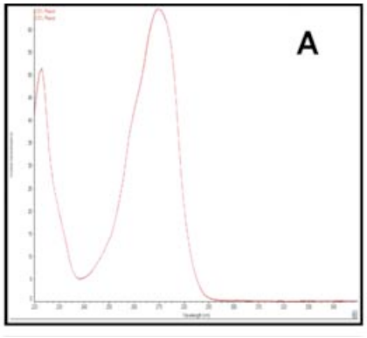
\includegraphics[height=2in]{./images/Nanodrop_A.pdf}
				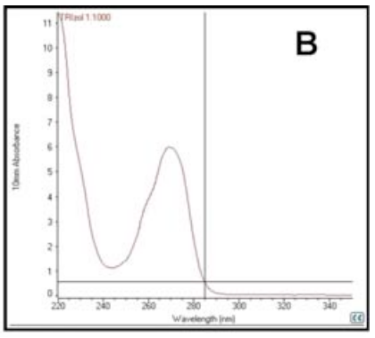
\includegraphics[height=2in]{./images/Nanodrop_B.pdf} \\
				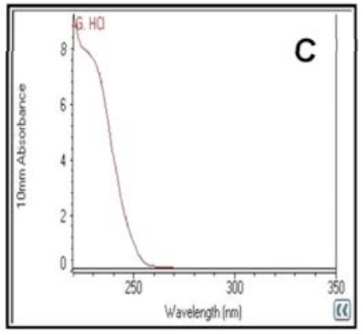
\includegraphics[height=2in]{./images/Nanodrop_C.pdf}
				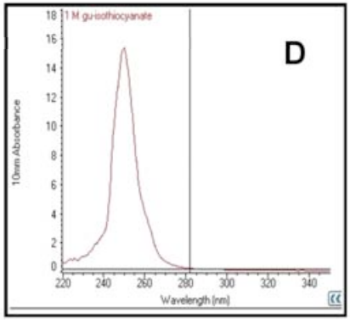
\includegraphics[height=2in]{./images/Nanodrop_D.pdf}
			\end{center}
			\caption {Spectra of reagents used in the isolation of nucleic acids. A) TriZol, B) Phenol, C) Guanidine HCL and D) Guanidinium isocyanate.}
		\end{figure}	

	\newpage

		\begin{figure}[h]
			\begin{center}
				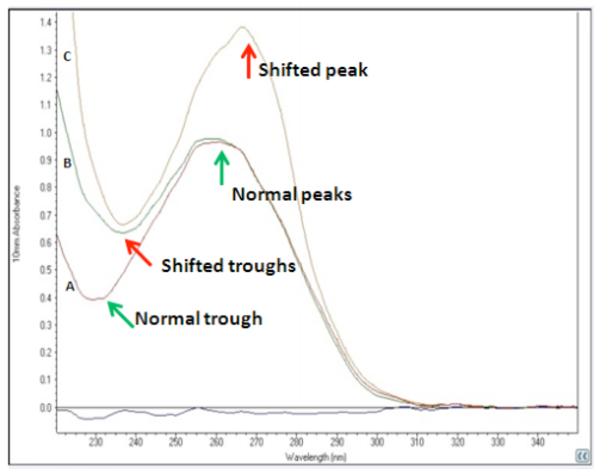
\includegraphics[height=2in]{./images/Nanodrop_peaks.pdf}
			\end{center}
			\caption{Spectra of purified DNA without contamination (A), and of the same DNA sample contaminated with guanidine (B) and phenol (C).}
		\end{figure}
	
	\newpage
	
	\subsection{Quality and quantity assessment of DNA and RNA with Qubit}

		\vspace{5mm}
	
	
		\noindent No data are currently available addressing the mutagenicity or toxicity of the Qubit BR reagents. This reagent is known to bind nucleic 		acid. Treat the Qubit BR reagent with the same safety precautions as all other potential mutagens and dispose of the dye in accordance with local 		regulations. 
	
		\vspace{3mm}
	
		\noindent The Qubit has several kits based on the sample needs. Use the appropriate kit for your sample. Each kit has its own buffer, reagents, 		and standards; so follow the protocol below using the appropriate buffer, reagents, and standards for your sample.

		\vspace{3mm}

		\noindent If you have RNA and your samples are expected to give you 
		\begin{itemize}
			\item[--] a yield of 20 - 1000 ng, use the RNA BR Assay Kit. 
			\item[--] a yield of 0.2 - 100 ng, use the RNA HS Assay Kit. 
		\end{itemize}
		\noindent If you have DNA and your samples are expected to give you
		\begin{itemize}
			\item[--] a yield of 20 - 1000 ng, use the DNA BR Assay Kit. 
			\item[--] a yield of 0.2 - 100 ng, use the DNA HS Assay Kit.
		\end{itemize}
		
		\noindent Use filter tips for this procedure.
	
		\vspace{5mm}
	
		{\bf To do before you start}	
	
		\begin{itemize}
			\item Remove the standards from the 4$^{\circ}$C refrigerator and let them warm to room temperature for 15-30 min. Qubit reagents are 				sensitive to light, so keep the reagents in the dark. 
			\item Get an epi tube or falcon tube (depending on the quantity of samples that you will be working with) for mixing your working solution.
			\item Label your Qubit assay 0.5 ml tubes: 2 tubes for the standards and 1 tube per sample
			\item *** Use only thin-wall, clear 0.5 mL optical-grade real-time PCR tubes. Acceptable tubes include Qubit assay tubes (500 tubes, 				Invitrogen 	Cat. no. Q32856) or Axygen PCR-05-C tubes (VWR, part number 10011-830).
		\end{itemize}
		
		\vspace{5mm}
		
		\noindent {\bf Protocol}

		\begin{enumerate}
			\item Get standards from refrigerator. Let them warm to room temperature
			\item Make the working solution for the samples and 2 standards by diluting the reagent and the BR buffer in 1:200 ratio.  Use a clean plastic 			tube each time you make working solution. Do not mix the working solution in a glass container. For example, for 8 samples, prepare enough 			working solution for the samples and 2 standards: $\sim$200 uL per tube in 10 tubes yields 2 mL of working solution (10 uL of reagent plus 			1990 uL of buffer).
		
			\begin{table}[h]
				\centering
				\begin{tabular}{| c | c |}
				\hline
				\cellcolor{gray}{\bf Reagent} & \cellcolor{gray}{\bf Number of samples 1X (uL)}  \\
				\hline
				Reagent (RNA BR, or DNA BR, or DNA HS & 1 uL \\
				BR buffer (RNA BR, or DNA BR. or  DNA HS) & 199 uL \\
				\hline
				\end{tabular}
			\end{table}

			\item Prepare standard 1 and standard 2 by mixing 190 uL working solution and 10 uK of standard 1 or standard 2 in 0.5 mL tubes. Vortex 2-3 			seconds, being careful not to create bubbles. 
		
			\begin{table}[h]
				\centering
				\begin{tabular}{| c | c |}
				\hline
				\cellcolor{gray}{\bf Reagent} & \cellcolor{gray}{\bf Number of samples 1X (uL)}  \\
				\hline
				Working Solution (RNA BR, or DNA BR, or DNA HS & 190 uL \\
				Standard 1 (RNA BR, or DNA BR. or  DNA HS) & 10 uL \\
				\hline
				\end{tabular}
			\end{table}

			\begin{table}[h]
				\centering
				\begin{tabular}{| c | c |}
				\hline
				\cellcolor{gray}{\bf Reagent} & \cellcolor{gray}{\bf Number of samples 1X (uL)}  \\
				\hline
				Working Solution (RNA BR, or DNA BR, or DNA HS & 190 uL \\
				Standard 2 (RNA BR, or DNA BR. or  DNA HS) & 10 uL \\
				\hline
				\end{tabular}
			\end{table}

			\noindent{\bf Note:} Careful pipetting is critical to ensure that exactly 10 uL of each standard is added to the 190 uL of working solution. 
		
			\item Prepare the samples by mixing 199 uL of the working solution with 1uL of sample (RNA or DNA) in 0.5 mL tubes and mix by vortexing 			2-3 seconds. Repeat this step for every sample that you have. 
		
			\begin{table}[H]
				\centering
				\begin{tabular}{| c | c |}
				\hline
				\cellcolor{gray}{\bf Reagent} & \cellcolor{gray}{\bf Number of samples 1X (uL)}  \\
				\hline
				Working Solution (RNA BR, or DNA BR, or DNA HS & 199 uL \\
				Sample (RNA or DNA) & 1 uL \\
				\hline
				\end{tabular}
			\end{table}
		
			\noindent {\bf Note:} If samples are suspected to be low in concentration, then use up to 20 ul of sample and adjust the working solution 				volume so the overall volume of the mix remains 200 uL. 		

		\end{enumerate}
	
	\newpage 
	
	\subsection{Homemade Magnetic Beads (SpeedBeads)}
	
		B.Faircloth \& T.Glenn et al. 2011 \\
		\url{<https://ethanomics.files.wordpress.com/2012/08/serapure_v2-2.pdf>}

		\vspace{5mm}

		\noindent {\bf Reagents}
		
		\begin{itemize}
			\itemsep0mm
			\item Sera-mag SpeedBeads (Fisher\# 09-981-123)
			\item PEG-8000 (Amresco 0159)
			\item 0.5 M EDTA pH 8.0 (Amresco E177)
			\item 1.0 M Tris, pH 8.0 (Amresco E199)
			\item Tween 20 (Amresco 0777)
			\item 5 M NaCL
			\item Fermentas ladder(s) (Ultra low range: Fisher \# FERSM1211, 50bp: FERSM0371)
			\item Rare earth magnet stand (Ambion AM10055 or NEB S1506S)
			\item TE
		\end{itemize}

		\vspace{3mm}
		
		\noindent{\bf Protocol part 1:}
		
		\begin{enumerate}	
			\item Transfer 500 uL SpeedBeads to microfuge tube (Sera-Mag SpeedBeads \#65152105050250)
			\item Collect beads in magnetic stand. Wash the beads two times with 500 uL TE. Remove the microcentrifuge from the magnetic stand to do 			the wash and the bring back the tube to the magnetic stand to remove the wash. 
			\item Resuspend in 500 uL TE *do not add the resuspended beads until the last part of the part 2 protocol
		\end{enumerate}
		
		\vspace{3mm}
		
		\noindent{\bf Protocol part 2:}
		
			\begin{enumerate}
				\itemsep0mm
				\item Add to a 50 mL tube:
				\begin{itemize}
					\item 4.5g PEG-8000 	(Amresco \#97061-102)
					\item 5 mL 5M NaCl
					\item 250 uL 1M Tris pH 8
					\item 50 uL 0.5M EDTA
					\item add sterile water to $\sim$24ml
					\item mix until PEG dissolves (vortex vigorously for a few minutes)
				\end{itemize}	
				\item add 137.5 uL 10\% Tween-20 or add 13.75 uL of Tween 20 to conical and mix gently
				\item Add 500 uL of the washed SpeedBeads from part 1
				\item Add TE or water to 50 mL 
			\end{enumerate}
		
		\vspace{3mm}
		
		\noindent{\bf Protocol part 3:}
		
		\vspace{3mm}
		
		\noindent You should test the Serapure mixture to ensure that it is working as expected. You can do this using DNA ladder (Fermentas GeneRuler - 		NEB ladders may cause problems):
		
		\begin{enumerate}
			\itemsep0mm
			\item Prep fresh aliquots of 70\% EtOH
			\item Mix 2 uL GeneRuler with 18 uL dH20
			\item Add 20 uL GeneRuler mixture to a volume of Serapure and/or AMPure (the specific volume depends on whether you are trying to 				exclude small fragments or not). 
			\item Incubate mixture 5 min. at room temperature. 
			\item Place on magnet stand
			\item Remove supernatant
			\item Add 500 uL 70\% EtOH
			\item Incubate on stand for 1 min
			\item Remove supernatant. 
			\item Add 500 uL 70\% EtOH
			\item Incubate on stand for 1 min
			\item Remove supernatant
			\item Place beads on 37$^{\circ}$C heat block for 3-4 min until dry
			\item Rehydrate with 20 uL H20
			\item Place on magnet stand
			\item Transfer supernatant to new tube
			\item Mix supernatant with 1 uL loading dye. 
			\item Electrophorese in 1.5\% agarose for 60 min at 100V
		\end{enumerate}
		
		\vspace{3mm}
		
		\noindent The following image from the Faircloth protocol compares the results of "purifying" a mix of 2 uL Fermentas Ultra Low Range Ladder + 		18 uL dH20 using several different amounts of AMPure or Serapure solution to DNA solution. AMPure is on the left, "Serapure" is on the right. After 		preparing 20 uL of ladder + water mix, we combined that with the volumes of AMPure or Serapure listed below and then purified using the standard 		protocol: 
		
		\begin{figure}[H]
			\begin{center}
				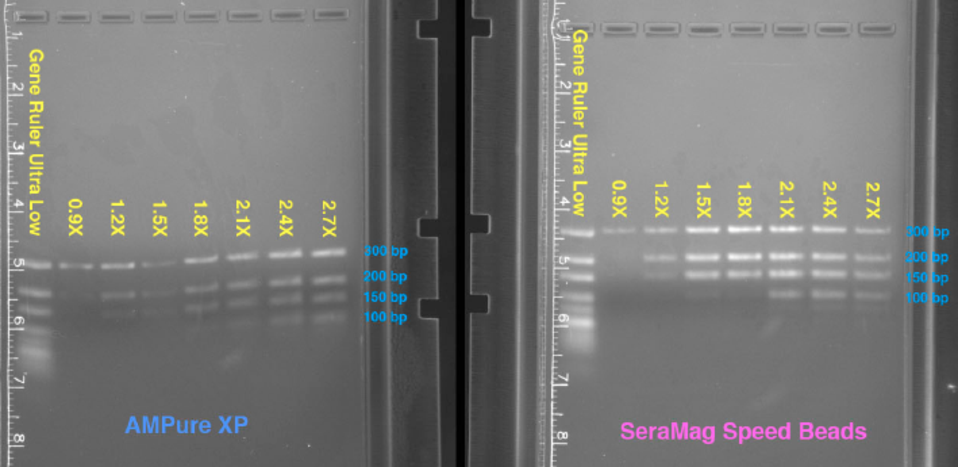
\includegraphics[height=2in]{./images/SpeedBeads_gel.pdf}
			\end{center}
		\end{figure}
		
		\noindent As you can see, the volume of AMPure or SeraPure controls the size of fragments recovered. More specifically, it is the ratio of PEG 			solution used to the volume of the DNA in solution which makes the difference, not the count of beads in solution (provided they are above the 			minimum level). This is what makes it possible to do "double-SPRI" size selection. 
		
	\newpage
	
	\subsection{DNA Bead Wash with pre-made Speed Beads}
	
	\noindent Adapted from Agencourt AMPure XP PCR Purification protocol
	
	\vspace{3mm}
	
	\noindent The homemade beads for this protocol should be prepared prior the procedure detail in this protocol. We will refer to the aliquots of pre-made	Speed Beads as DNA beads. Please look in section 10.3 for a protocol on how to prepare Speed Beads. This protocol can be used for samples in plate 	or in 	individual epitubes. 
	
	\vspace{3mm}
	
	{\bf Protocol}
	
	\begin{enumerate}
		\itemsep0mm
		\item Shake the aliquots of DNA beads (pre-made Speed Beads) to Resuspend any magnetic particles that may have settled. 
		\item Add 1.8X volume of DNA beads to the sample. For example add 180 uL of DNA beads to a sample of a 100 uL volume. 
		\item Mix reagent and sample thoroughly by pipette mixing 10 times. Let the mixed samples incubate 5 minutes at room temperature for maximum 		recovery.  
		\item Place the reaction plate onto a magnetic plate for 2 minutes to separate beads from solution. Wait for the solution to clear before proceeding 		to the next step.
		\item While the reaction tube or plate are situated in the magnet plate, aspire the cleared solution from the reaction plate and discard. Leave 5 uL of 		supernatant behind, otherwise beads are drawn out with the supernatant. 
		\item While the reaction tube or plate are situated in the magnet plate, dispense 200 uL of 70\% ethanol to each well of the reaction plate and 			incubate for 30 seconds at room temperature. Aspirate the ethanol and discard. If the total volume of sample plus reagent exceeds 200 uL, then 		use a wash volume of at least the volume of sample plus reagent. 
		\item Remove the reaction plate from the magnet plate, and then add 40 uL of elution buffer to each well of the reaction plate and pipette mix 10 		times. Incubate for 2 minutes. The liquid level will be high enough to contact the magnetic beads at a 40 uL elution volume. A greater volume of 		elution buffer can be used, but using less than 40 uL will require extra mixing (to ensure the liquid comes into contact with the beads, and may not 		be sufficient to elute the entire PCR product. If you are wishing for a higher DNA concentration use a lower elution volume than the initial sample 		volume. 
		\item Place the reaction plate/tube back in the magnetic plate for 1 minute to separate beads from the solution. 
		\item Transfer the eluate to a new plate/tube. 
	\end{enumerate}
	
	\begin{adjustwidth}{0.25in}{0pt}{\bf Note:} Bead carryover into the final plate is usually not a cause for concern. The samples can be stored in the freezer 	with beads and the beads are inert in downstream enzymatic reactions. If bead carryover must be limited for any reason, 2 uL - 5 uL of eluate can be left 	behind the original plate. In addition, a second transfer away from the beads is optional. To do so, place the final plate containing beads and eluate onto 	the magnet for 1 minute to separate the beads. Transfer the eluate into another clean plate. \end{adjustwidth}

\newpage

	\subsection{Resuspend Primer Stocks \label{Resuspend_Primer_Stocks}}

		Adapted from the California Academy of Science Protocol
	
		\vspace{3mm}
	
		{\bf Primer resuspension}	
		
		\begin{enumerate}
			\item Briefly vortex and centrifuge primer stocks when they arrive. The dry pellet may have become dislodged from the bottom of the tube. 
			\item Label the top of the lids of the primer vial. It will help in future efforts of working with the primer. 
			\item Oligos can be resuspended in Milli-Q water or 1X TE buffer. TE buffer would keep the quality of the oligos for longer. Calculate the 				amount of TE buffer or water needed to be added to bring the primer to a 100uM concentration. You can multiply the nmol quantity amount, 			noted in the primer data sheet, by 10. This primer is now your main stock, and you should only use the main stock to make working stocks of 			the primer.
			\item For example, if your primer`s nmol quantity is 36, you should add 360 uL of TE buffer to the tube. This will give you a final stock 				concentration of 100uM.  
			\item Vortex the primer at low speed a couple of times and let the primer sit for at least 5 minutes before use. 
			\item Do a quick spin to the primer tube sand store the primers in the -20 freezer or make working stocks for future use. 
		\end{enumerate}
		
		\vspace{3mm}
		
		{\bf Preparing work stocks from primers main stock 10 uM}
		
		\begin{enumerate}
			\item. PCR reactions tend to require 10 uM oligos stock. Label a 0.5 mL or 1.5 mL tubes per primer or primer mix. It is better to make a few 			working stocks at once. 
			\item To each tube add 90 uL of Milli-Q water
			\item Add 10 uL of primer stock. Quick vortex and quick spin. The 10 uM primers now can be stored in the freezer. 
		\end{enumerate}
		
	\newpage
 
	
	
		
\end{document}